%%%%%%%%%%%%%%%%%%%%%%%%%%%%%%%%%%%%%%%%%%%%%%%%%%%%%%%%%%%%%%%%%%%%%%%%%%%%%%%%
% Preámbulo                                                                    %
%%%%%%%%%%%%%%%%%%%%%%%%%%%%%%%%%%%%%%%%%%%%%%%%%%%%%%%%%%%%%%%%%%%%%%%%%%%%%%%%

\documentclass[11pt,a4paper,titlepage,twoside,openright,openbib]{report}

%%% RELACIÓN DE VARIABLES A PERSONALIZAR %%%
\def\lingua{esp} % descomenta esta liña se redactarás a memoria en español
\def\nome{Alonso Rodriguez Iglesias}                             % substitúe aquí o teu nome
\def\nomedirectorA{Juan Touriño Domínguez}             % substitúe aquí o nome de quen dirixe
\def\nomedirectorB{María José Martín Santamaría}             % substitúe aquí o nome de quen dirixe
\def\titulo{Diseño e implementación hardware y software de un mini-supercomputador con Raspberry Pi} % substitúe aquí o título do teu TFG
\def\mencion{ENXEÑARÍA DE COMPUTADORES}

%\def\renomearcadros{si} % descomenta esta liña se redactas a memoria en español e prefires que
                         % os "cuadros" e o "índice de cuadros" se renomeen
                         % a "tablas" e "índice de tablas" respectivamente

\usepackage{estilo_tfg}

% Lista de paquetes potencialmente interesantes (uso baixo demanda)

\usepackage[all]{nowidow}
% \usepackage{alltt}       % proporciona o entorno alltt, semellante a verbatim pero que respecta comandos
% \usepackage{enumitem}    % permite personalizar os entornos de lista
% \usepackage{eurofont}    % proporciona o comando \euro
\usepackage{float}       % permite máis opcións para controlar obxectos flotantes (táboas, figuras)
% \usepackage{hhline}      % permie personalizar as liñas horizontais en arrays e táboas
% \usepackage{longtable}   % permite construir táboas que ocupan máis dunha páxina
\usepackage{lscape}      % permite colocar partes do documento en orientación apaisada
% \usepackage{moreverb}    % permite personalizar o entorno verbatim
% \usepackage{multirow}    % permite crear celdas que ocupan varias filas da mesma táboa
\usepackage{pdfpages}    % permite insertar ficheiros en PDF no documento
\usepackage{rotating}    % permite diferentes tipos de rotacións para figuras e táboas
% \usepackage{subcaption}  % permite a inclusión de varias subfiguras nunha figura
% \usepackage{tabu}        % permite táboas flexibles
% \usepackage{tabularx}    % permite táboas con columnas de anchura determinada

\usepackage{sourcecodepro}
\usepackage{pgfplots}
\usepackage{pgfplotstable}
\pgfplotsset{compat = newest}
\usepackage{wrapfig}
\usepackage{etoolbox}
\BeforeBeginEnvironment{wrapfigure}{\setlength{\intextsep}{0pt}}
\usepackage{svg}
\usepackage{adjustbox}
\newcommand{\vasymptote}[2][]{
    \draw [thick,ficblue,densely dashed,#1] ({rel axis cs:0,0} -| {axis cs:#2,0}) -- ({rel axis cs:0,1} -| {axis cs:#2,0});
}
\pgfplotsset{every axis/.append style={
        scaled y ticks = false, 
        scaled x ticks = false, 
        y tick label style={/pgf/number format/.cd, fixed},
        x tick label style={/pgf/number format/.cd, fixed}
    }
}

%%%%%%%%%%%%%%%%%%%%%%%%%%%%%%%%%%%%%%%%%%%%%%%%%%%%%%%%%%%%%%%%%%%%%%%%%%%%%%%%
% Corpo                                                                        %
%%%%%%%%%%%%%%%%%%%%%%%%%%%%%%%%%%%%%%%%%%%%%%%%%%%%%%%%%%%%%%%%%%%%%%%%%%%%%%%%

\begin{document}

%%%%%%%%%%%%%%%%%%%%%%%%%%%%%%%%%%%%%%%%
% Preliminares do documento            %
%%%%%%%%%%%%%%%%%%%%%%%%%%%%%%%%%%%%%%%%

\begin{titlepage}
  
  \hspace*{128pt}
  \textcolor{udcpink}{{\fontencoding{T1}\fontfamily{phv}\selectfont Facultade de Informática}}\\[-32pt]

  \begin{center}
    
\includegraphics[scale=0.3]{imaxes/udc}\\[35pt]

    {\large TRABALLO FIN DE GRAO \\
            GRAO EN ENXEÑARÍA INFORMÁTICA \\
            MENCIÓN EN \mencion } \\[100pt]
    
    \begin{huge}
      \begin{spacing}{1.3}
        \bfseries \titulo
      \end{spacing}
    \end{huge}
  \end{center}
  
  \vfill
  
  \begin{flushright}
    {\large
    \begin{tabular}{ll}
      {\bf Estudante:} & \nome \\
      {\bf Dirección:} & \nomedirectorA \\ % COPIA E PEGA ESTA LIÑA MÁIS VECES SE O PRECISAS
      {\bf Dirección:} & \nomedirectorB \\ % COPIA E PEGA ESTA LIÑA MÁIS VECES SE O PRECISAS
    \end{tabular}}
  \end{flushright}
  \rightline{A Coruña, \today.}
\end{titlepage}

\paxinaenbranco
\dedicatoria{Dedicatoria} % escribe neste comando o teu texto de dedicatoria
\paxinaenbranco
\paxinaenbranco
\begin{agradecementos}
\blindtext                % substitúe este comando polo teu texto de agradecementos
\end{agradecementos}
\paxinaenbranco
%%%%%%%%%%%%%%%%%%%%%%%%%%%%%%%%%%%%%%%%%%%%%%%%%%%%%%%%%%%%%%%%%%%%%%%%%%%%%%%%

\begin{abstract}\thispagestyle{empty}
  \blindtext % substitúe este comando polo resumo do teu TFG
             % na lingua principal do documento (tipicamente: galego)

  \vspace*{25pt}
  \begin{segundoresumo}
    \blindtext % substitúe este comando polo resumo do teu TFG
               % na lingua secundaria do documento (tipicamente: inglés)
  \end{segundoresumo}
\vspace*{25pt}
\begin{multicols}{2}
\begin{description}
\item [\palabraschaveprincipal:] \mbox{} \\[-20pt]
  \blindlist{itemize}[7] % substitúe este comando por un itemize
                         % que relacione as palabras chave
                         % que mellor identifiquen o teu TFG
                         % no idioma principal da memoria (tipicamente: galego)
\end{description}
\begin{description}
\item [\palabraschavesecundaria:] \mbox{} \\[-20pt]
  \blindlist{itemize}[7] % substitúe este comando por un itemize
                         % que relacione as palabras chave
                         % que mellor identifiquen o teu TFG
                         % no idioma secundario da memoria (tipicamente: inglés)
\end{description}
\end{multicols}

\end{abstract}

%%%%%%%%%%%%%%%%%%%%%%%%%%%%%%%%%%%%%%%%%%%%%%%%%%%%%%%%%%%%%%%%%%%%%%%%%%%%%%%%

\paxinaenbranco

\pagenumbering{roman}
\setcounter{page}{1}
\bstctlcite{IEEEexample:BSTcontrol}

\tableofcontents
\listoffigures
\listoftables
\cleardoublepage

\pagenumbering{arabic}
\setcounter{page}{1}

%%%%%%%%%%%%%%%%%%%%%%%%%%%%%%%%%%%%%%%%
% Capítulos                            %
%%%%%%%%%%%%%%%%%%%%%%%%%%%%%%%%%%%%%%%%

\chapter{Introdución}
\label{chap:introducion}

\lettrine{P}{rimer} capítulo da memoria, onde xeralmente se exporán as
liñas mestras do traballo, os obxectivos, etc. Incluimos un par de
exemplos de citas~\cite{ErlangBook,ErlangWebBook} e de referencias
internas (sección \ref{sec:mostra}, páxina \pageref{sec:mostra}).

\Blindtext

\section{Sección de mostra}
\label{sec:mostra}

\Blindtext

\subsection{Subsección de mostra}

\Blindtext

%\include{contido/...}
% Analisis -> Diseño -> Implementación -> Testeo
\chapter{Clúpiter: Conceptos básicos}
\label{chap:conceptos_basicos}

\lettrine{P}{ara} comprender el objetivo del proyecto y su propuesta de valor, primero es necesario entender sus características, la justificación de las mismas, y el funcionamiento de sus componentes más primitivos.

\section{Nombre y marca corporativa}
Si bien este no es un elemento altamente importante en un proyecto de ingeniería como este, si que es conveniente, y nunca está de más, otorgarle personalidad mediante la creación de un nombre e isotipo para el mismo.

El nombre del clúster es \textbf{Clúpiter} (ClúPIter): una mezcla entre las palabras ``Clúster'' y el ``PI'' de la \acrlong{rpi}, que de forma muy conveniente recuerda en su segunda parte a Júpiter. Este es a su vez planeta del sistema solar junto con el (enano) Plutón, nombre del clúster del \acrshort{gac}\footnote{\url{http://pluton.dec.udc.es}} (\acrlong{gac}). Es cuanto menos paradógico que el clúster en miniatura sea Júpiter, y el real sea Plutón\dots

En cuanto a la marca del clúster, éste no puede quedar sin un logo, que se muestra en la Figura \ref{fig:clupiter_logo}.\footnote{El uso del logo de Arch Linux sin autorización explícita está permitido en general para propósitos no comerciales. Clúpiter no tiene ningún tipo de vinculación con la marca Arch Linux (\url{https://wiki.archlinux.org/title/DeveloperWiki:TrademarkPolicy})}

\begin{figure}[h!]
  \centering
  \vspace*{0.5cm}
  \def\svgwidth{0.50\textwidth}
  \input{pdf_tex/clupiter_logo/clupiter_logo.pdf_tex}
  \caption{Logo de Clúpiter}
  \label{fig:clupiter_logo}
\end{figure}

\section{Clústeres}
Los clústeres, de los que para este proyecto se tratarán los de alto rendimiento, son conjuntos de ordenadores diseñados para ofrecer altas prestaciones de cálculo.

Estos clústeres pueden ser homogéneos o heterogéneos, siendo compuestos por computadores con la misma arquitectura y capacidades, o con arquitecturas o capacidades diferentes, respectivamente.

En el caso de Clúpiter, éste es un clúster muy homogéneo, ya que está compuesto por ocho mini-computadores exactamente iguales.

Existen multitud de amateurs y amantes de la informática que como proyecto personal deciden montar un clúster de \acrlong{rpi}s, entre los que por ejemplo se encuentra Jeff Geerling\footnote{\url{https://www.youtube.com/user/geerlingguy}}, un famoso YouTuber del cual uno de sus proyectos se puede encontrar en la Figura \ref{fig:cluster-pi-ejemplo}.

\begin{figure}[h!]
  \centering
  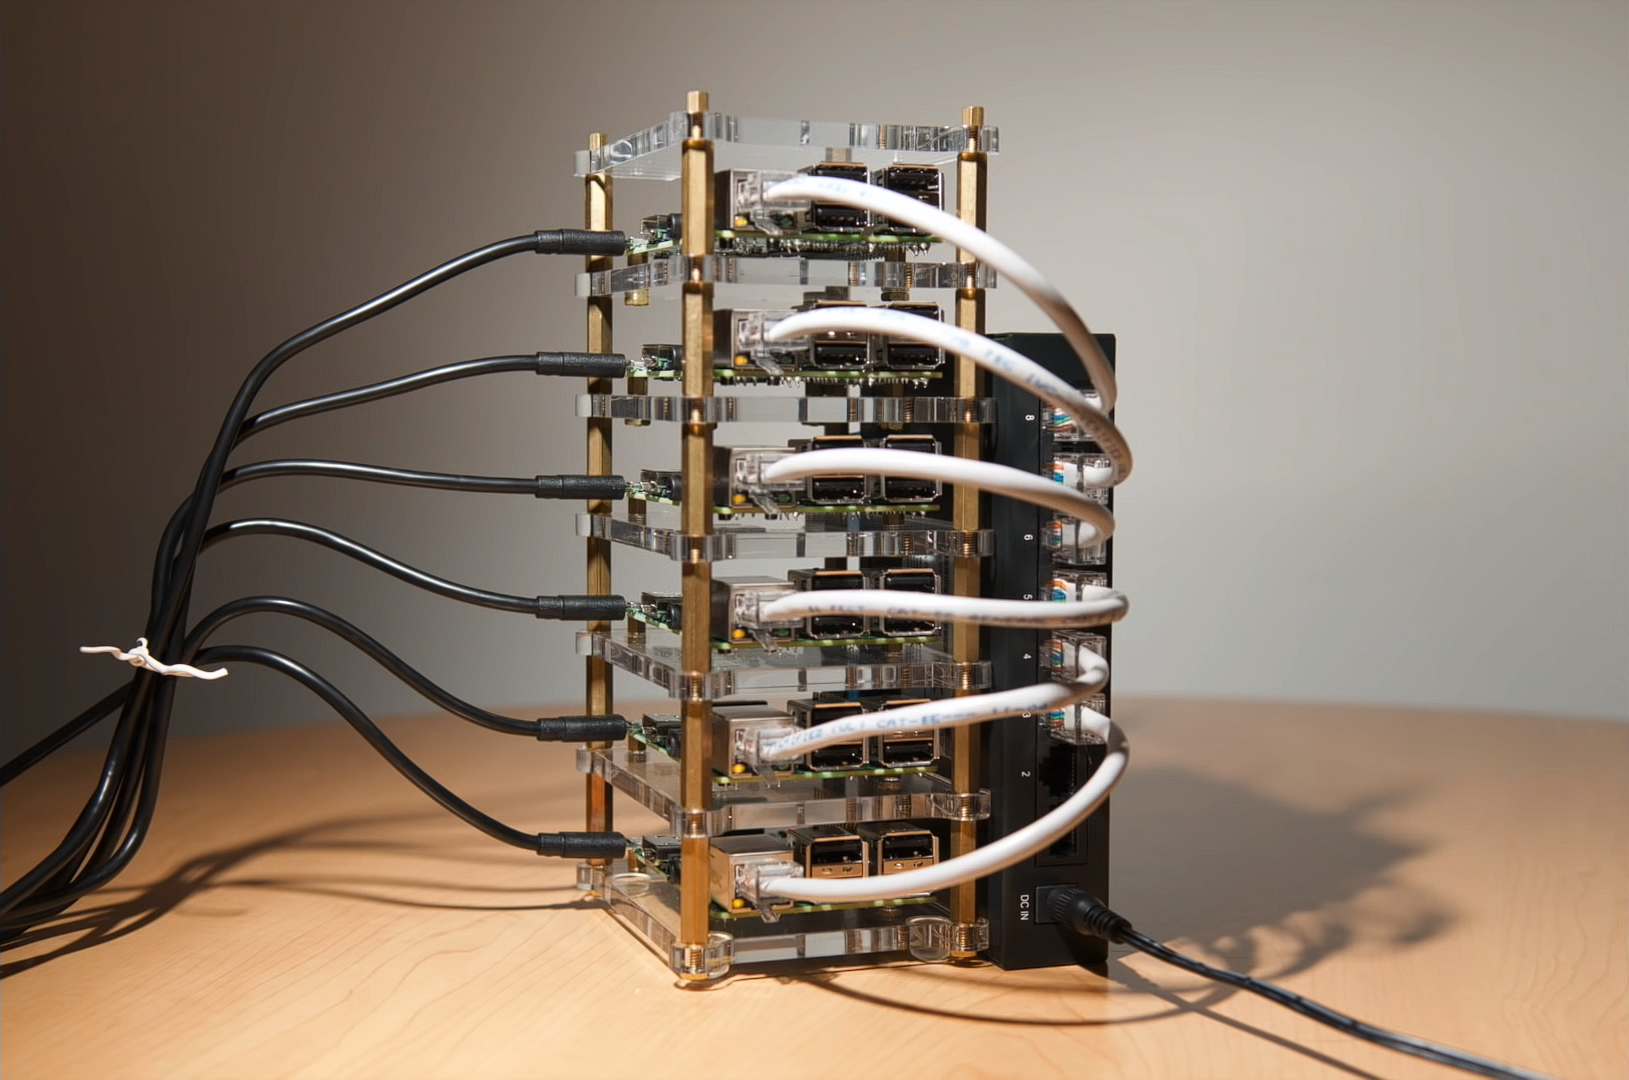
\includegraphics[width=0.75\textwidth]{img/cluster-pi-home.png}
  \caption{Mini-clúster casero basado en \acrlong{rpi} 3\cite{geerling_intro_cluster}}
  \label{fig:cluster-pi-ejemplo}
\end{figure}

Además, en el mundo académico también ha habido aproximaciones similares al trabajo desarrollado, destacando \textit{Wee Archie}, un clúster de 18 \acrlong{rpi} 2 que, como se puede leer en la página web del proyecto \cite{wee_archie_webpage}, pretende emular el comportamiento de un supercomputador real, el supercomputador ARCHER\footnote{\url{https://www.archer.ac.uk}} (Figura \ref{fig:wee_archie_girl}).

\begin{figure}[h!]
  \centering
  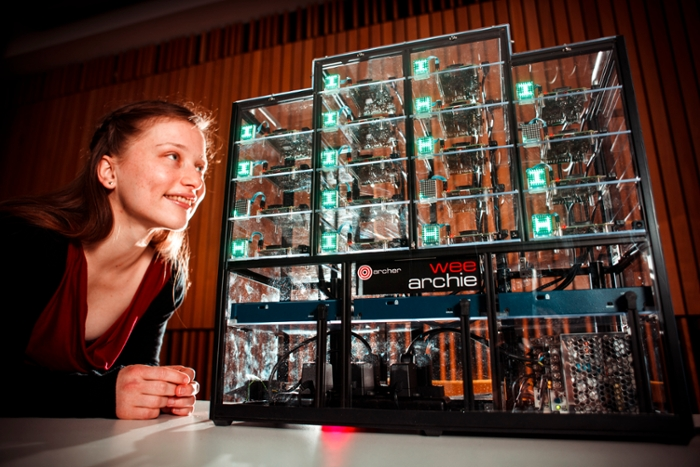
\includegraphics[width=0.75\textwidth]{img/wee-girl.jpg}
  \caption{Mini-supercomputador Wee Archie}
  \label{fig:wee_archie_girl}
\end{figure}

\section{Raspberry Pi 4 Model B}
\label{sec:raspberry_pi_4_model_b}
Cada aproximadamente dos años, la Raspberry Pi Foundation saca una nueva versión de su compacto y más exitoso producto: la \acrlong{rpi}, o por sus siglas \acrshort{rpi}. Estos pequeños computadores vienen en diversos formatos de forma, pero el que ha catapultado esta plataforma al éxito ha sido el formato que denominan \textit{Standard}\footnote{85.6 mm × 56.5 mm}.

\begin{figure}[h!]
  \centering
  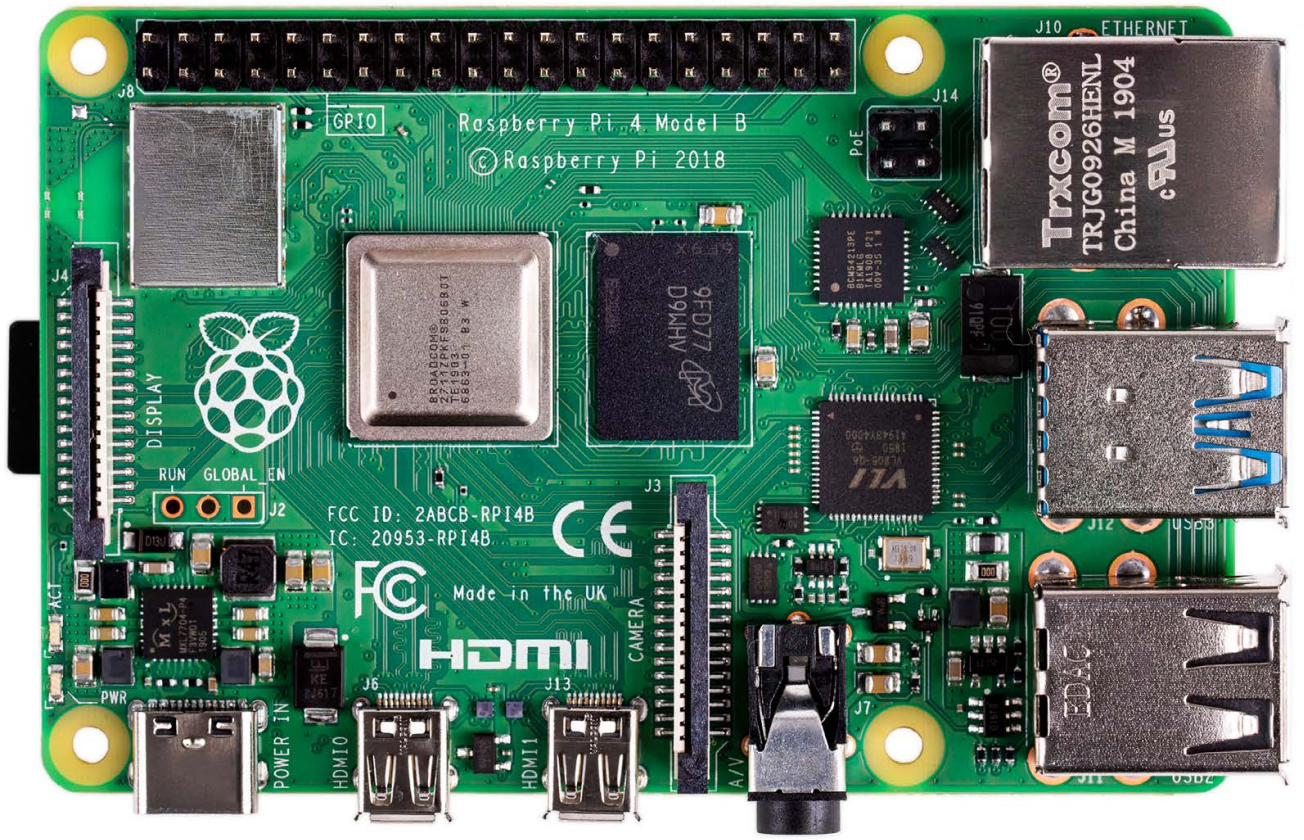
\includegraphics[width=0.75\textwidth]{img/rpi_parts/rpi_base.jpg}
  \caption{\acrlong{rpi} 4 Model B}
  \label{fig:rpi_base}
\end{figure}

Siendo cada versión mucho más potente que la anterior, y costando aproximadamente el mismo precio, está claro que la Raspberry Pi Foundation está haciendo un excelente trabajo aportando valor a este segmento del bajo consumo y coste.

La \acrlong{rpi} 4B (4 Model B), que se muestra en la Figura \ref{fig:rpi_base}, es la versión más nueva de formato \textit{Standard}, y por ello ha sido la elección para constituir la base del clúster. A continuación se muestran sus principales características \cite{rpi4b_specifications}:

\subsection{CPU}
La \acrshort{cpu} (\textit{\acrlong{cpu}} o Unidad de Procesamiento Central) de este nuevo modelo es la \textbf{Broadcom BCM2711}, un procesador con arquitectura ARMv8-A y 4 núcleos Cortex-A72, que funcionan a 1.5GHz.

Estos núcleos cuentan con un \textit{pipeline} de 15 etapas, ejecución OOO (\textit{out-of-order}) y predictor de saltos, entre otros.

Además, cuenta con 48KB de L1I y 32KB de L1D por núcleo, así como 1MB de L2 compartido (256KB por núcleo). Esto emparejado con un único chip de 2GB de memoria LPDDR4-3200, es suficiente para un uso doméstico sencillo, pero quizás no sea la mejor disposición para el cómputo intensivo como se verá más adelante.
% TODO INSERTAR REF?????

\subsection{GPU/VPU}
\label{ssec:gpu_vpu}
A pesar de que el integrado que se muestra en la foto del apartado superior es un \acrshort{soc} (\textit{\acrlong{soc}}), se ha preferido tratar la \acrshort{cpu} y la \acrshort{gpu}/\acrshort{vpu} (\textit{\acrlong{gpu}}/\textit{\acrlong{vpu}}) por separado. Y es que los gráficos integrados de esta última \acrlong{rpi} son una importante mejora sobre la VideoCore IV que equipaban modelos anteriores.

La GPU en la \acrshort{rpi}4 es la VideoCore VI, y cuenta con multitud de soporte para multimedia y una potencia gráfica aceptable. En concreto, acelera por hardware H.265 (4Kp60 decode), H.264 (1080p60 decode, 1080p30 encode), y soporta OpenGL ES, 3.0.

Además, y lo que considero más interesante, es que posteriormente al lanzamiento se comenzó para esta gráfica el desarrollo de un driver de Vulkan: un estándar abierto de última generación para programación de gráficos, pero que también se puede emplear para cómputo. Esto es una fantástica noticia, ya que permite acelerar ciertas cargas de trabajo aprovechando la inmensa capacidad de cómputo paralelo de estos dispositivos, siendo una de las más habituales en estos dispositivos la transformada de Fourier.

Realizar algún tipo de programa para computación \acrshort{gpgpu} (\textit{\acrlong{gpgpu}}) en Vulkan queda fuera de lo que pretende abarcar este trabajo, pero es un interesante proyecto para la realización de alguna otra iteración sobre esta plataforma.

\subsection{E/S}
En términos de \acrlong{e-s} (\acrshort{e-s}) la \acrshort{rpi}4B cuenta con multitud de puertos, de los que se van a utilizar Gigabit Ethernet y USB 3.0. Sin embargo, éste equipa de serie otros muchos otros puertos en los pines \acrshort{gpio} (\acrlong{gpio}), cuya disposición se puede encontrar en la Figura \ref{fig:rpi_gpio_pinout}, y que es un estándar de-facto, ya que es la misma para todos los modelos de \acrlong{rpi} y otros dispositivos similares, que la adoptan para mayor inter-compatibilidad.

Los puertos y protocolos que integra la \acrlong{rpi} en el \acrshort{gpio} son algunos como I2C (\textit{Inter-Integrated Circuit}), UART (\textit{Universal Asynchronous Receiver-Transmitter}), SPI (\textit{Serial Peripheral Interface}) y video compuesto, así como mútiples pines de alimentación a 5 y 3.3V. Por último, ya en la propia placa, tambien se dispone de un puerto DSI (\textit{Display Serial Interface}) y CSI (\textit{Camera Serial Interface}), y dos salidas de vídeo HDMI.

También cuenta con interfaz de datos inalámbrica, que soporta tecnologías WiFi 802.11.b/g/n/ac y Bluetooth 5.0.

\begin{figure}[h!]
  \centering
  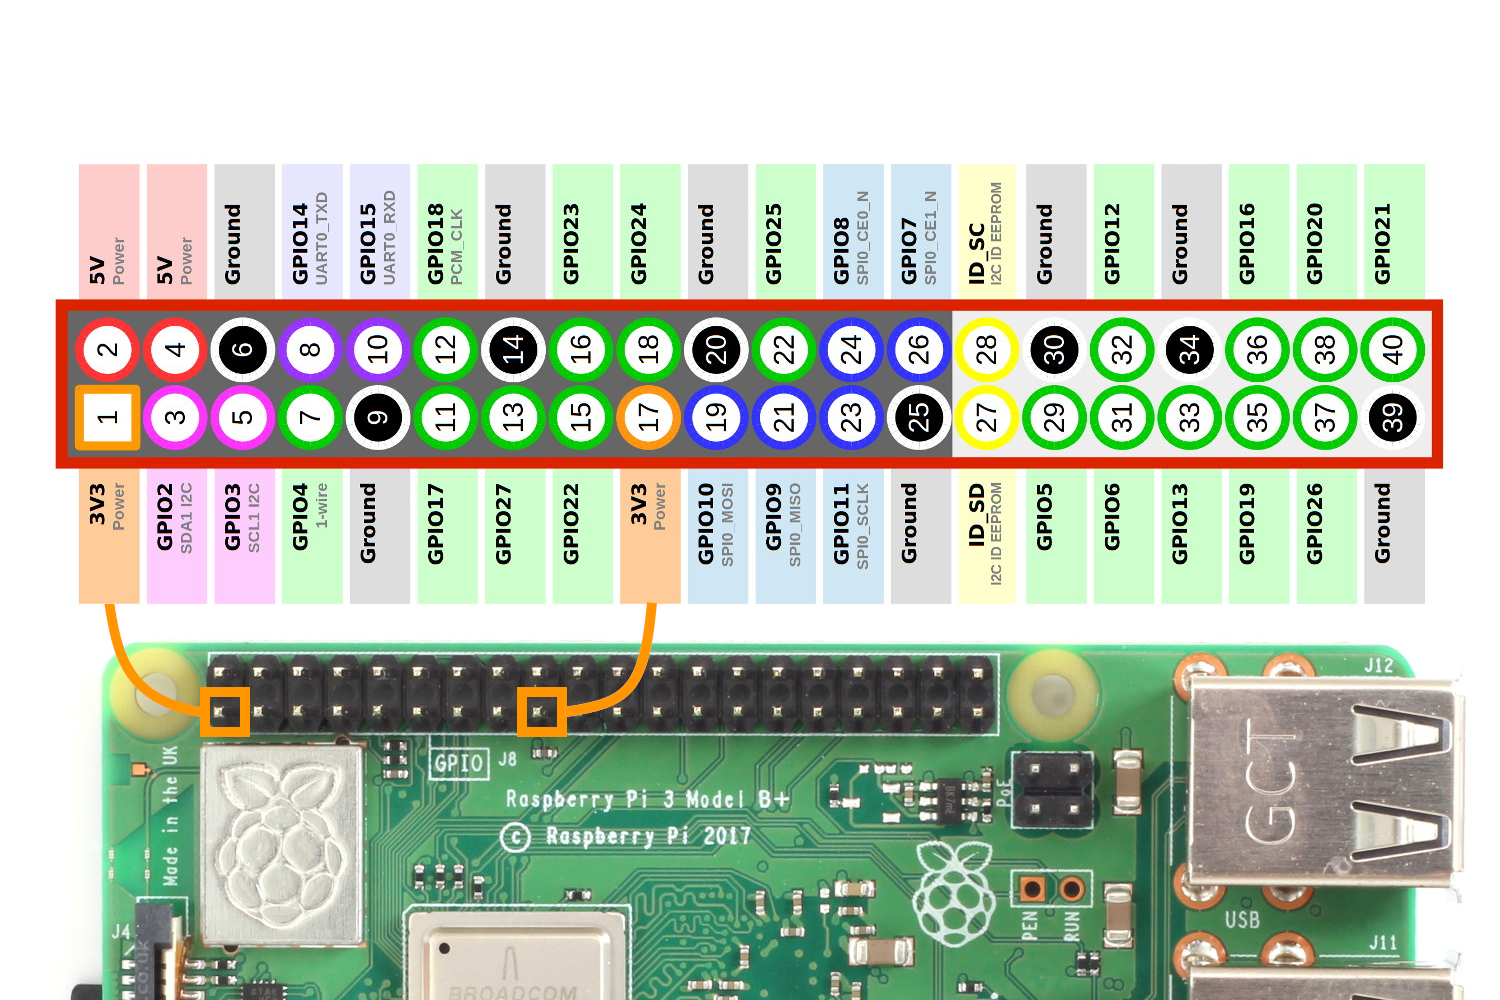
\includegraphics[width=0.85\textwidth]{img/rpi_parts/rpi_gpio.png}
  \caption{Pines GPIO de la \acrlong{rpi} 4}
  \label{fig:rpi_gpio_pinout}
\end{figure}

\section{MPI}
Para aprovechar todo el potencial hardware de los supercomputadores y, en general, de los computadores paralelos, existen paradigmas de programación específicos. \acrshort{mpi} (\acrlong{mpi})\footnote{\url{https://www.mpi-forum.org}} es un estándar para la programación de los sistemas paralelos de memoria distribuida como Clúpiter. Es una especificación de paso de mensajes que define la sintaxis y semántica del conjunto de rutinas para comunicar datos entre procesos que exponen las diferentes implementaciones. 

Entre las implementaciones disponibles, las más utilizadas son:
\begin{itemize}
  \item\textbf{OpenMPI}\footnote{\url{https://www.open-mpi.org}}: Implementación libre mantenida por un consorcio de académicos, investigadores y socios que ofrece elevada eficiencia y flexibilidad a quien la implementa. Además, es la librería \acrshort{mpi} que ofrece Arch Linux (distribución Linux de Clúpiter) en sus repositorios oficiales, y contra la que se compilan por defecto sus ejecutables.
  \item\textbf{MPICH}\footnote{\url{https://www.mpich.org}}: Otra implementación libre de MPI muy similar a OpenMPI en rendimiento, flexibilidad y modo de desarrollo.
  \item\textbf{Intel MPI}\footnote{\url{https://software.intel.com/content/www/us/en/develop/tools/oneapi/components/mpi-library.html}}: Implementación propietaria de \acrshort{mpi} por parte de Intel. Está especializada en productos de la propia marca y optimizaza para ellos, por lo que suele arrojar un mayor rendimiento que las contrapartes libres.
\end{itemize}

La base de \acrshort{mpi} son las primitivas de envío y recepción de datos. Existen dos funciones de envío y recepción \textbf{síncronas} (esto es, la llamada a la función solamente termina cuando todos los miembros involucrados en la ejecución de dicha función han terminado):
\begin{itemize}
  \item \textbf{MPI\_Send}: Envía un mensaje a destino, y espera a que el receptor esté listo para recibirlo. 
  \item \textbf{MPI\_Recv}: Espera a que llegue un mensaje del origen, y cuando éste está listo para enviarlo, lo recibe.
\end{itemize}

Estas funciones tienen su contraparte para programación asíncrona, que puede arrojar un mayor rendimiento, pero también requiere un extra de complejidad y puede no ser trivial. Las funciones básicas para realizar programación asíncrona con \acrshort{mpi} son \textbf{MPI\_Isend} y \textbf{MPI\_Irecv}. A su vez son necesarias para chequear el estado de la ejecución asíncrona las funciones \textbf{MPI\_Test} (asíncrona) y \textbf{MPI\_Wait} (síncrona).

Otra funcionalidad de \acrshort{mpi} ampliamente utilizada son las primitivas de grupo u operaciones colectivas, las cuales permiten la comunicación entre más de 2 procesos.

Las colectivas más sencillas y comunes de MPI son las siguientes \cite{cheung_mpi}:
\begin{itemize}
  \item \textbf{MPI\_Bcast}: Emite (hace \textit{broadcast}) el mensaje a todos los procesos del comunicador, tal y como se muestra en la Figura \ref{fig:mpi_bcast}.
  
  \begin{figure}[H]
    \vspace*{0.5cm}
    \centering
    \resizebox {0.8\textwidth} {!} {
    % Created by Eps2pgf 0.7.0 (build on 2008-08-24) on Sun Aug 22 14:08:15 CEST 2021
\begin{pgfpicture}
\pgfpathmoveto{\pgfqpoint{0cm}{0cm}}
\pgfpathlineto{\pgfqpoint{25.188cm}{0cm}}
\pgfpathlineto{\pgfqpoint{25.188cm}{10.724cm}}
\pgfpathlineto{\pgfqpoint{0cm}{10.724cm}}
\pgfpathclose
\pgfusepath{clip}
\begin{pgfscope}
\pgfpathmoveto{\pgfqpoint{0cm}{10.724cm}}
\pgfpathlineto{\pgfqpoint{0cm}{0cm}}
\pgfpathlineto{\pgfqpoint{25.188cm}{0cm}}
\pgfpathlineto{\pgfqpoint{25.188cm}{10.724cm}}
\pgfpathclose
\pgfusepath{clip}
\begin{pgfscope}
\begin{pgfscope}
\definecolor{eps2pgf_color}{rgb}{1,1,0}\pgfsetstrokecolor{eps2pgf_color}\pgfsetfillcolor{eps2pgf_color}
\pgfpathmoveto{\pgfqpoint{5.429cm}{5.92cm}}
\pgfpathlineto{\pgfqpoint{17.97cm}{5.92cm}}
\pgfpathlineto{\pgfqpoint{17.97cm}{4.173cm}}
\pgfpathlineto{\pgfqpoint{5.429cm}{4.173cm}}
\pgfpathclose
\pgfseteorule\pgfusepath{fill}\pgfsetnonzerorule
\end{pgfscope}
\begin{pgfscope}
\pgfsetdash{}{0cm}
\pgfsetlinewidth{0.317mm}
\definecolor{eps2pgf_color}{rgb}{1,1,0}\pgfsetstrokecolor{eps2pgf_color}\pgfsetfillcolor{eps2pgf_color}
\pgfpathmoveto{\pgfqpoint{5.429cm}{5.92cm}}
\pgfpathlineto{\pgfqpoint{17.97cm}{5.92cm}}
\pgfpathlineto{\pgfqpoint{17.97cm}{4.173cm}}
\pgfpathlineto{\pgfqpoint{5.429cm}{4.173cm}}
\pgfpathclose
\pgfusepath{stroke}
\end{pgfscope}
\begin{pgfscope}
\definecolor{eps2pgf_color}{rgb}{0.53,0.81,1}\pgfsetstrokecolor{eps2pgf_color}\pgfsetfillcolor{eps2pgf_color}
\pgfpathmoveto{\pgfqpoint{2.73cm}{9.095cm}}
\pgfpathlineto{\pgfqpoint{3.524cm}{9.095cm}}
\pgfpathlineto{\pgfqpoint{3.524cm}{8.301cm}}
\pgfpathlineto{\pgfqpoint{2.73cm}{8.301cm}}
\pgfpathclose
\pgfseteorule\pgfusepath{fill}\pgfsetnonzerorule
\end{pgfscope}
\begin{pgfscope}
\pgfsetdash{}{0cm}
\pgfsetlinewidth{0.317mm}
\definecolor{eps2pgf_color}{gray}{0}\pgfsetstrokecolor{eps2pgf_color}\pgfsetfillcolor{eps2pgf_color}
\pgfpathmoveto{\pgfqpoint{2.73cm}{9.095cm}}
\pgfpathlineto{\pgfqpoint{3.524cm}{9.095cm}}
\pgfpathlineto{\pgfqpoint{3.524cm}{8.301cm}}
\pgfpathlineto{\pgfqpoint{2.73cm}{8.301cm}}
\pgfpathclose
\pgfusepath{stroke}
\end{pgfscope}
\begin{pgfscope}
\definecolor{eps2pgf_color}{rgb}{0,1,0}\pgfsetstrokecolor{eps2pgf_color}\pgfsetfillcolor{eps2pgf_color}
\pgfpathmoveto{\pgfqpoint{3.524cm}{9.095cm}}
\pgfpathlineto{\pgfqpoint{4.318cm}{9.095cm}}
\pgfpathlineto{\pgfqpoint{4.318cm}{8.301cm}}
\pgfpathlineto{\pgfqpoint{3.524cm}{8.301cm}}
\pgfpathclose
\pgfseteorule\pgfusepath{fill}\pgfsetnonzerorule
\end{pgfscope}
\begin{pgfscope}
\pgfsetdash{}{0cm}
\pgfsetlinewidth{0.317mm}
\definecolor{eps2pgf_color}{gray}{0}\pgfsetstrokecolor{eps2pgf_color}\pgfsetfillcolor{eps2pgf_color}
\pgfpathmoveto{\pgfqpoint{3.524cm}{9.095cm}}
\pgfpathlineto{\pgfqpoint{4.318cm}{9.095cm}}
\pgfpathlineto{\pgfqpoint{4.318cm}{8.301cm}}
\pgfpathlineto{\pgfqpoint{3.524cm}{8.301cm}}
\pgfpathclose
\pgfusepath{stroke}
\end{pgfscope}
\begin{pgfscope}
\definecolor{eps2pgf_color}{rgb}{1,1,0}\pgfsetstrokecolor{eps2pgf_color}\pgfsetfillcolor{eps2pgf_color}
\pgfpathmoveto{\pgfqpoint{1.937cm}{9.095cm}}
\pgfpathlineto{\pgfqpoint{2.73cm}{9.095cm}}
\pgfpathlineto{\pgfqpoint{2.73cm}{8.301cm}}
\pgfpathlineto{\pgfqpoint{1.937cm}{8.301cm}}
\pgfpathclose
\pgfseteorule\pgfusepath{fill}\pgfsetnonzerorule
\end{pgfscope}
\begin{pgfscope}
\pgfsetdash{}{0cm}
\pgfsetlinewidth{0.317mm}
\definecolor{eps2pgf_color}{gray}{0}\pgfsetstrokecolor{eps2pgf_color}\pgfsetfillcolor{eps2pgf_color}
\pgfpathmoveto{\pgfqpoint{1.937cm}{9.095cm}}
\pgfpathlineto{\pgfqpoint{2.73cm}{9.095cm}}
\pgfpathlineto{\pgfqpoint{2.73cm}{8.301cm}}
\pgfpathlineto{\pgfqpoint{1.937cm}{8.301cm}}
\pgfpathclose
\pgfusepath{stroke}
\end{pgfscope}
\begin{pgfscope}
\definecolor{eps2pgf_color}{rgb}{1,0.75,0.75}\pgfsetstrokecolor{eps2pgf_color}\pgfsetfillcolor{eps2pgf_color}
\pgfpathmoveto{\pgfqpoint{4.318cm}{9.095cm}}
\pgfpathlineto{\pgfqpoint{5.112cm}{9.095cm}}
\pgfpathlineto{\pgfqpoint{5.112cm}{8.301cm}}
\pgfpathlineto{\pgfqpoint{4.318cm}{8.301cm}}
\pgfpathclose
\pgfseteorule\pgfusepath{fill}\pgfsetnonzerorule
\end{pgfscope}
\begin{pgfscope}
\pgfsetdash{}{0cm}
\pgfsetlinewidth{0.317mm}
\definecolor{eps2pgf_color}{gray}{0}\pgfsetstrokecolor{eps2pgf_color}\pgfsetfillcolor{eps2pgf_color}
\pgfpathmoveto{\pgfqpoint{4.318cm}{9.095cm}}
\pgfpathlineto{\pgfqpoint{5.112cm}{9.095cm}}
\pgfpathlineto{\pgfqpoint{5.112cm}{8.301cm}}
\pgfpathlineto{\pgfqpoint{4.318cm}{8.301cm}}
\pgfpathclose
\pgfusepath{stroke}
\end{pgfscope}
\begin{pgfscope}
\definecolor{eps2pgf_color}{rgb}{0.53,0.81,1}\pgfsetstrokecolor{eps2pgf_color}\pgfsetfillcolor{eps2pgf_color}
\pgfpathmoveto{\pgfqpoint{2.889cm}{1.157cm}}
\pgfpathlineto{\pgfqpoint{3.683cm}{1.157cm}}
\pgfpathlineto{\pgfqpoint{3.683cm}{0.363cm}}
\pgfpathlineto{\pgfqpoint{2.889cm}{0.363cm}}
\pgfpathclose
\pgfseteorule\pgfusepath{fill}\pgfsetnonzerorule
\end{pgfscope}
\begin{pgfscope}
\pgfsetdash{}{0cm}
\pgfsetlinewidth{0.317mm}
\definecolor{eps2pgf_color}{gray}{0}\pgfsetstrokecolor{eps2pgf_color}\pgfsetfillcolor{eps2pgf_color}
\pgfpathmoveto{\pgfqpoint{2.889cm}{1.157cm}}
\pgfpathlineto{\pgfqpoint{3.683cm}{1.157cm}}
\pgfpathlineto{\pgfqpoint{3.683cm}{0.363cm}}
\pgfpathlineto{\pgfqpoint{2.889cm}{0.363cm}}
\pgfpathclose
\pgfusepath{stroke}
\end{pgfscope}
\begin{pgfscope}
\definecolor{eps2pgf_color}{rgb}{0,1,0}\pgfsetstrokecolor{eps2pgf_color}\pgfsetfillcolor{eps2pgf_color}
\pgfpathmoveto{\pgfqpoint{3.683cm}{1.157cm}}
\pgfpathlineto{\pgfqpoint{4.477cm}{1.157cm}}
\pgfpathlineto{\pgfqpoint{4.477cm}{0.363cm}}
\pgfpathlineto{\pgfqpoint{3.683cm}{0.363cm}}
\pgfpathclose
\pgfseteorule\pgfusepath{fill}\pgfsetnonzerorule
\end{pgfscope}
\begin{pgfscope}
\pgfsetdash{}{0cm}
\pgfsetlinewidth{0.317mm}
\definecolor{eps2pgf_color}{gray}{0}\pgfsetstrokecolor{eps2pgf_color}\pgfsetfillcolor{eps2pgf_color}
\pgfpathmoveto{\pgfqpoint{3.683cm}{1.157cm}}
\pgfpathlineto{\pgfqpoint{4.477cm}{1.157cm}}
\pgfpathlineto{\pgfqpoint{4.477cm}{0.363cm}}
\pgfpathlineto{\pgfqpoint{3.683cm}{0.363cm}}
\pgfpathclose
\pgfusepath{stroke}
\end{pgfscope}
\begin{pgfscope}
\definecolor{eps2pgf_color}{rgb}{1,1,0}\pgfsetstrokecolor{eps2pgf_color}\pgfsetfillcolor{eps2pgf_color}
\pgfpathmoveto{\pgfqpoint{2.095cm}{1.157cm}}
\pgfpathlineto{\pgfqpoint{2.889cm}{1.157cm}}
\pgfpathlineto{\pgfqpoint{2.889cm}{0.363cm}}
\pgfpathlineto{\pgfqpoint{2.095cm}{0.363cm}}
\pgfpathclose
\pgfseteorule\pgfusepath{fill}\pgfsetnonzerorule
\end{pgfscope}
\begin{pgfscope}
\pgfsetdash{}{0cm}
\pgfsetlinewidth{0.317mm}
\definecolor{eps2pgf_color}{gray}{0}\pgfsetstrokecolor{eps2pgf_color}\pgfsetfillcolor{eps2pgf_color}
\pgfpathmoveto{\pgfqpoint{2.095cm}{1.157cm}}
\pgfpathlineto{\pgfqpoint{2.889cm}{1.157cm}}
\pgfpathlineto{\pgfqpoint{2.889cm}{0.363cm}}
\pgfpathlineto{\pgfqpoint{2.095cm}{0.363cm}}
\pgfpathclose
\pgfusepath{stroke}
\end{pgfscope}
\begin{pgfscope}
\definecolor{eps2pgf_color}{rgb}{1,0.75,0.75}\pgfsetstrokecolor{eps2pgf_color}\pgfsetfillcolor{eps2pgf_color}
\pgfpathmoveto{\pgfqpoint{4.477cm}{1.157cm}}
\pgfpathlineto{\pgfqpoint{5.27cm}{1.157cm}}
\pgfpathlineto{\pgfqpoint{5.27cm}{0.363cm}}
\pgfpathlineto{\pgfqpoint{4.477cm}{0.363cm}}
\pgfpathclose
\pgfseteorule\pgfusepath{fill}\pgfsetnonzerorule
\end{pgfscope}
\begin{pgfscope}
\pgfsetdash{}{0cm}
\pgfsetlinewidth{0.317mm}
\definecolor{eps2pgf_color}{gray}{0}\pgfsetstrokecolor{eps2pgf_color}\pgfsetfillcolor{eps2pgf_color}
\pgfpathmoveto{\pgfqpoint{4.477cm}{1.157cm}}
\pgfpathlineto{\pgfqpoint{5.27cm}{1.157cm}}
\pgfpathlineto{\pgfqpoint{5.27cm}{0.363cm}}
\pgfpathlineto{\pgfqpoint{4.477cm}{0.363cm}}
\pgfpathclose
\pgfusepath{stroke}
\end{pgfscope}
\begin{pgfscope}
\definecolor{eps2pgf_color}{rgb}{0.53,0.81,1}\pgfsetstrokecolor{eps2pgf_color}\pgfsetfillcolor{eps2pgf_color}
\pgfpathmoveto{\pgfqpoint{9.557cm}{1.316cm}}
\pgfpathlineto{\pgfqpoint{10.35cm}{1.316cm}}
\pgfpathlineto{\pgfqpoint{10.35cm}{0.522cm}}
\pgfpathlineto{\pgfqpoint{9.557cm}{0.522cm}}
\pgfpathclose
\pgfseteorule\pgfusepath{fill}\pgfsetnonzerorule
\end{pgfscope}
\begin{pgfscope}
\pgfsetdash{}{0cm}
\pgfsetlinewidth{0.317mm}
\definecolor{eps2pgf_color}{gray}{0}\pgfsetstrokecolor{eps2pgf_color}\pgfsetfillcolor{eps2pgf_color}
\pgfpathmoveto{\pgfqpoint{9.557cm}{1.316cm}}
\pgfpathlineto{\pgfqpoint{10.35cm}{1.316cm}}
\pgfpathlineto{\pgfqpoint{10.35cm}{0.522cm}}
\pgfpathlineto{\pgfqpoint{9.557cm}{0.522cm}}
\pgfpathclose
\pgfusepath{stroke}
\end{pgfscope}
\begin{pgfscope}
\definecolor{eps2pgf_color}{rgb}{0,1,0}\pgfsetstrokecolor{eps2pgf_color}\pgfsetfillcolor{eps2pgf_color}
\pgfpathmoveto{\pgfqpoint{10.35cm}{1.316cm}}
\pgfpathlineto{\pgfqpoint{11.144cm}{1.316cm}}
\pgfpathlineto{\pgfqpoint{11.144cm}{0.522cm}}
\pgfpathlineto{\pgfqpoint{10.35cm}{0.522cm}}
\pgfpathclose
\pgfseteorule\pgfusepath{fill}\pgfsetnonzerorule
\end{pgfscope}
\begin{pgfscope}
\pgfsetdash{}{0cm}
\pgfsetlinewidth{0.317mm}
\definecolor{eps2pgf_color}{gray}{0}\pgfsetstrokecolor{eps2pgf_color}\pgfsetfillcolor{eps2pgf_color}
\pgfpathmoveto{\pgfqpoint{10.35cm}{1.316cm}}
\pgfpathlineto{\pgfqpoint{11.144cm}{1.316cm}}
\pgfpathlineto{\pgfqpoint{11.144cm}{0.522cm}}
\pgfpathlineto{\pgfqpoint{10.35cm}{0.522cm}}
\pgfpathclose
\pgfusepath{stroke}
\end{pgfscope}
\begin{pgfscope}
\definecolor{eps2pgf_color}{rgb}{1,1,0}\pgfsetstrokecolor{eps2pgf_color}\pgfsetfillcolor{eps2pgf_color}
\pgfpathmoveto{\pgfqpoint{8.763cm}{1.316cm}}
\pgfpathlineto{\pgfqpoint{9.557cm}{1.316cm}}
\pgfpathlineto{\pgfqpoint{9.557cm}{0.522cm}}
\pgfpathlineto{\pgfqpoint{8.763cm}{0.522cm}}
\pgfpathclose
\pgfseteorule\pgfusepath{fill}\pgfsetnonzerorule
\end{pgfscope}
\begin{pgfscope}
\pgfsetdash{}{0cm}
\pgfsetlinewidth{0.317mm}
\definecolor{eps2pgf_color}{gray}{0}\pgfsetstrokecolor{eps2pgf_color}\pgfsetfillcolor{eps2pgf_color}
\pgfpathmoveto{\pgfqpoint{8.763cm}{1.316cm}}
\pgfpathlineto{\pgfqpoint{9.557cm}{1.316cm}}
\pgfpathlineto{\pgfqpoint{9.557cm}{0.522cm}}
\pgfpathlineto{\pgfqpoint{8.763cm}{0.522cm}}
\pgfpathclose
\pgfusepath{stroke}
\end{pgfscope}
\begin{pgfscope}
\definecolor{eps2pgf_color}{rgb}{1,0.75,0.75}\pgfsetstrokecolor{eps2pgf_color}\pgfsetfillcolor{eps2pgf_color}
\pgfpathmoveto{\pgfqpoint{11.144cm}{1.316cm}}
\pgfpathlineto{\pgfqpoint{11.938cm}{1.316cm}}
\pgfpathlineto{\pgfqpoint{11.938cm}{0.522cm}}
\pgfpathlineto{\pgfqpoint{11.144cm}{0.522cm}}
\pgfpathclose
\pgfseteorule\pgfusepath{fill}\pgfsetnonzerorule
\end{pgfscope}
\begin{pgfscope}
\pgfsetdash{}{0cm}
\pgfsetlinewidth{0.317mm}
\definecolor{eps2pgf_color}{gray}{0}\pgfsetstrokecolor{eps2pgf_color}\pgfsetfillcolor{eps2pgf_color}
\pgfpathmoveto{\pgfqpoint{11.144cm}{1.316cm}}
\pgfpathlineto{\pgfqpoint{11.938cm}{1.316cm}}
\pgfpathlineto{\pgfqpoint{11.938cm}{0.522cm}}
\pgfpathlineto{\pgfqpoint{11.144cm}{0.522cm}}
\pgfpathclose
\pgfusepath{stroke}
\end{pgfscope}
\begin{pgfscope}
\definecolor{eps2pgf_color}{rgb}{0.53,0.81,1}\pgfsetstrokecolor{eps2pgf_color}\pgfsetfillcolor{eps2pgf_color}
\pgfpathmoveto{\pgfqpoint{15.907cm}{1.316cm}}
\pgfpathlineto{\pgfqpoint{16.7cm}{1.316cm}}
\pgfpathlineto{\pgfqpoint{16.7cm}{0.522cm}}
\pgfpathlineto{\pgfqpoint{15.907cm}{0.522cm}}
\pgfpathclose
\pgfseteorule\pgfusepath{fill}\pgfsetnonzerorule
\end{pgfscope}
\begin{pgfscope}
\pgfsetdash{}{0cm}
\pgfsetlinewidth{0.317mm}
\definecolor{eps2pgf_color}{gray}{0}\pgfsetstrokecolor{eps2pgf_color}\pgfsetfillcolor{eps2pgf_color}
\pgfpathmoveto{\pgfqpoint{15.907cm}{1.316cm}}
\pgfpathlineto{\pgfqpoint{16.7cm}{1.316cm}}
\pgfpathlineto{\pgfqpoint{16.7cm}{0.522cm}}
\pgfpathlineto{\pgfqpoint{15.907cm}{0.522cm}}
\pgfpathclose
\pgfusepath{stroke}
\end{pgfscope}
\begin{pgfscope}
\definecolor{eps2pgf_color}{rgb}{0,1,0}\pgfsetstrokecolor{eps2pgf_color}\pgfsetfillcolor{eps2pgf_color}
\pgfpathmoveto{\pgfqpoint{16.7cm}{1.316cm}}
\pgfpathlineto{\pgfqpoint{17.494cm}{1.316cm}}
\pgfpathlineto{\pgfqpoint{17.494cm}{0.522cm}}
\pgfpathlineto{\pgfqpoint{16.7cm}{0.522cm}}
\pgfpathclose
\pgfseteorule\pgfusepath{fill}\pgfsetnonzerorule
\end{pgfscope}
\begin{pgfscope}
\pgfsetdash{}{0cm}
\pgfsetlinewidth{0.317mm}
\definecolor{eps2pgf_color}{gray}{0}\pgfsetstrokecolor{eps2pgf_color}\pgfsetfillcolor{eps2pgf_color}
\pgfpathmoveto{\pgfqpoint{16.7cm}{1.316cm}}
\pgfpathlineto{\pgfqpoint{17.494cm}{1.316cm}}
\pgfpathlineto{\pgfqpoint{17.494cm}{0.522cm}}
\pgfpathlineto{\pgfqpoint{16.7cm}{0.522cm}}
\pgfpathclose
\pgfusepath{stroke}
\end{pgfscope}
\begin{pgfscope}
\definecolor{eps2pgf_color}{rgb}{1,1,0}\pgfsetstrokecolor{eps2pgf_color}\pgfsetfillcolor{eps2pgf_color}
\pgfpathmoveto{\pgfqpoint{15.113cm}{1.316cm}}
\pgfpathlineto{\pgfqpoint{15.907cm}{1.316cm}}
\pgfpathlineto{\pgfqpoint{15.907cm}{0.522cm}}
\pgfpathlineto{\pgfqpoint{15.113cm}{0.522cm}}
\pgfpathclose
\pgfseteorule\pgfusepath{fill}\pgfsetnonzerorule
\end{pgfscope}
\begin{pgfscope}
\pgfsetdash{}{0cm}
\pgfsetlinewidth{0.317mm}
\definecolor{eps2pgf_color}{gray}{0}\pgfsetstrokecolor{eps2pgf_color}\pgfsetfillcolor{eps2pgf_color}
\pgfpathmoveto{\pgfqpoint{15.113cm}{1.316cm}}
\pgfpathlineto{\pgfqpoint{15.907cm}{1.316cm}}
\pgfpathlineto{\pgfqpoint{15.907cm}{0.522cm}}
\pgfpathlineto{\pgfqpoint{15.113cm}{0.522cm}}
\pgfpathclose
\pgfusepath{stroke}
\end{pgfscope}
\begin{pgfscope}
\definecolor{eps2pgf_color}{rgb}{1,0.75,0.75}\pgfsetstrokecolor{eps2pgf_color}\pgfsetfillcolor{eps2pgf_color}
\pgfpathmoveto{\pgfqpoint{17.494cm}{1.316cm}}
\pgfpathlineto{\pgfqpoint{18.288cm}{1.316cm}}
\pgfpathlineto{\pgfqpoint{18.288cm}{0.522cm}}
\pgfpathlineto{\pgfqpoint{17.494cm}{0.522cm}}
\pgfpathclose
\pgfseteorule\pgfusepath{fill}\pgfsetnonzerorule
\end{pgfscope}
\begin{pgfscope}
\pgfsetdash{}{0cm}
\pgfsetlinewidth{0.317mm}
\definecolor{eps2pgf_color}{gray}{0}\pgfsetstrokecolor{eps2pgf_color}\pgfsetfillcolor{eps2pgf_color}
\pgfpathmoveto{\pgfqpoint{17.494cm}{1.316cm}}
\pgfpathlineto{\pgfqpoint{18.288cm}{1.316cm}}
\pgfpathlineto{\pgfqpoint{18.288cm}{0.522cm}}
\pgfpathlineto{\pgfqpoint{17.494cm}{0.522cm}}
\pgfpathclose
\pgfusepath{stroke}
\end{pgfscope}
\begin{pgfscope}
\definecolor{eps2pgf_color}{rgb}{0.53,0.81,1}\pgfsetstrokecolor{eps2pgf_color}\pgfsetfillcolor{eps2pgf_color}
\pgfpathmoveto{\pgfqpoint{22.415cm}{1.475cm}}
\pgfpathlineto{\pgfqpoint{23.209cm}{1.475cm}}
\pgfpathlineto{\pgfqpoint{23.209cm}{0.681cm}}
\pgfpathlineto{\pgfqpoint{22.415cm}{0.681cm}}
\pgfpathclose
\pgfseteorule\pgfusepath{fill}\pgfsetnonzerorule
\end{pgfscope}
\begin{pgfscope}
\pgfsetdash{}{0cm}
\pgfsetlinewidth{0.317mm}
\definecolor{eps2pgf_color}{gray}{0}\pgfsetstrokecolor{eps2pgf_color}\pgfsetfillcolor{eps2pgf_color}
\pgfpathmoveto{\pgfqpoint{22.415cm}{1.475cm}}
\pgfpathlineto{\pgfqpoint{23.209cm}{1.475cm}}
\pgfpathlineto{\pgfqpoint{23.209cm}{0.681cm}}
\pgfpathlineto{\pgfqpoint{22.415cm}{0.681cm}}
\pgfpathclose
\pgfusepath{stroke}
\end{pgfscope}
\begin{pgfscope}
\definecolor{eps2pgf_color}{rgb}{0,1,0}\pgfsetstrokecolor{eps2pgf_color}\pgfsetfillcolor{eps2pgf_color}
\pgfpathmoveto{\pgfqpoint{23.209cm}{1.475cm}}
\pgfpathlineto{\pgfqpoint{24.003cm}{1.475cm}}
\pgfpathlineto{\pgfqpoint{24.003cm}{0.681cm}}
\pgfpathlineto{\pgfqpoint{23.209cm}{0.681cm}}
\pgfpathclose
\pgfseteorule\pgfusepath{fill}\pgfsetnonzerorule
\end{pgfscope}
\begin{pgfscope}
\pgfsetdash{}{0cm}
\pgfsetlinewidth{0.317mm}
\definecolor{eps2pgf_color}{gray}{0}\pgfsetstrokecolor{eps2pgf_color}\pgfsetfillcolor{eps2pgf_color}
\pgfpathmoveto{\pgfqpoint{23.209cm}{1.475cm}}
\pgfpathlineto{\pgfqpoint{24.003cm}{1.475cm}}
\pgfpathlineto{\pgfqpoint{24.003cm}{0.681cm}}
\pgfpathlineto{\pgfqpoint{23.209cm}{0.681cm}}
\pgfpathclose
\pgfusepath{stroke}
\end{pgfscope}
\begin{pgfscope}
\definecolor{eps2pgf_color}{rgb}{1,1,0}\pgfsetstrokecolor{eps2pgf_color}\pgfsetfillcolor{eps2pgf_color}
\pgfpathmoveto{\pgfqpoint{21.622cm}{1.475cm}}
\pgfpathlineto{\pgfqpoint{22.415cm}{1.475cm}}
\pgfpathlineto{\pgfqpoint{22.415cm}{0.681cm}}
\pgfpathlineto{\pgfqpoint{21.622cm}{0.681cm}}
\pgfpathclose
\pgfseteorule\pgfusepath{fill}\pgfsetnonzerorule
\end{pgfscope}
\begin{pgfscope}
\pgfsetdash{}{0cm}
\pgfsetlinewidth{0.317mm}
\definecolor{eps2pgf_color}{gray}{0}\pgfsetstrokecolor{eps2pgf_color}\pgfsetfillcolor{eps2pgf_color}
\pgfpathmoveto{\pgfqpoint{21.622cm}{1.475cm}}
\pgfpathlineto{\pgfqpoint{22.415cm}{1.475cm}}
\pgfpathlineto{\pgfqpoint{22.415cm}{0.681cm}}
\pgfpathlineto{\pgfqpoint{21.622cm}{0.681cm}}
\pgfpathclose
\pgfusepath{stroke}
\end{pgfscope}
\begin{pgfscope}
\definecolor{eps2pgf_color}{rgb}{1,0.75,0.75}\pgfsetstrokecolor{eps2pgf_color}\pgfsetfillcolor{eps2pgf_color}
\pgfpathmoveto{\pgfqpoint{24.003cm}{1.475cm}}
\pgfpathlineto{\pgfqpoint{24.797cm}{1.475cm}}
\pgfpathlineto{\pgfqpoint{24.797cm}{0.681cm}}
\pgfpathlineto{\pgfqpoint{24.003cm}{0.681cm}}
\pgfpathclose
\pgfseteorule\pgfusepath{fill}\pgfsetnonzerorule
\end{pgfscope}
\begin{pgfscope}
\pgfsetdash{}{0cm}
\pgfsetlinewidth{0.317mm}
\definecolor{eps2pgf_color}{gray}{0}\pgfsetstrokecolor{eps2pgf_color}\pgfsetfillcolor{eps2pgf_color}
\pgfpathmoveto{\pgfqpoint{24.003cm}{1.475cm}}
\pgfpathlineto{\pgfqpoint{24.797cm}{1.475cm}}
\pgfpathlineto{\pgfqpoint{24.797cm}{0.681cm}}
\pgfpathlineto{\pgfqpoint{24.003cm}{0.681cm}}
\pgfpathclose
\pgfusepath{stroke}
\end{pgfscope}
\begin{pgfscope}
\definecolor{eps2pgf_color}{gray}{0}\pgfsetstrokecolor{eps2pgf_color}\pgfsetfillcolor{eps2pgf_color}
\pgftext[x=3.183cm,y=10.369cm,rotate=0]{\fontsize{27.1}{32.52}\selectfont{\textrm{\textbf{P}}}}
\end{pgfscope}
\begin{pgfscope}
\definecolor{eps2pgf_color}{gray}{0}\pgfsetstrokecolor{eps2pgf_color}\pgfsetfillcolor{eps2pgf_color}
\pgftext[x=3.556cm,y=9.987cm,rotate=0]{\fontsize{21.68}{26.02}\selectfont{\textrm{\textbf{0}}}}
\end{pgfscope}
\begin{pgfscope}
\definecolor{eps2pgf_color}{gray}{0}\pgfsetstrokecolor{eps2pgf_color}\pgfsetfillcolor{eps2pgf_color}
\pgftext[x=9.85cm,y=10.369cm,rotate=0]{\fontsize{27.1}{32.52}\selectfont{\textrm{\textbf{P}}}}
\end{pgfscope}
\begin{pgfscope}
\definecolor{eps2pgf_color}{gray}{0}\pgfsetstrokecolor{eps2pgf_color}\pgfsetfillcolor{eps2pgf_color}
\pgftext[x=10.226cm,y=10.15cm,rotate=0]{\fontsize{21.68}{26.02}\selectfont{\textrm{\textbf{1}}}}
\end{pgfscope}
\begin{pgfscope}
\definecolor{eps2pgf_color}{gray}{0}\pgfsetstrokecolor{eps2pgf_color}\pgfsetfillcolor{eps2pgf_color}
\pgftext[x=16.2cm,y=10.369cm,rotate=0]{\fontsize{27.1}{32.52}\selectfont{\textrm{\textbf{P}}}}
\end{pgfscope}
\begin{pgfscope}
\definecolor{eps2pgf_color}{gray}{0}\pgfsetstrokecolor{eps2pgf_color}\pgfsetfillcolor{eps2pgf_color}
\pgftext[x=16.572cm,y=9.992cm,rotate=0]{\fontsize{21.68}{26.02}\selectfont{\textrm{\textbf{2}}}}
\end{pgfscope}
\begin{pgfscope}
\definecolor{eps2pgf_color}{gray}{0}\pgfsetstrokecolor{eps2pgf_color}\pgfsetfillcolor{eps2pgf_color}
\pgftext[x=22.55cm,y=10.21cm,rotate=0]{\fontsize{27.1}{32.52}\selectfont{\textrm{\textbf{P}}}}
\end{pgfscope}
\begin{pgfscope}
\definecolor{eps2pgf_color}{gray}{0}\pgfsetstrokecolor{eps2pgf_color}\pgfsetfillcolor{eps2pgf_color}
\pgftext[x=22.917cm,y=9.986cm,rotate=0]{\fontsize{21.68}{26.02}\selectfont{\textrm{\textbf{3}}}}
\end{pgfscope}
\begin{pgfscope}
\pgfsetdash{}{0cm}
\pgfsetlinewidth{0.317mm}
\definecolor{eps2pgf_color}{gray}{0}\pgfsetstrokecolor{eps2pgf_color}\pgfsetfillcolor{eps2pgf_color}
\pgfpathmoveto{\pgfqpoint{1.619cm}{9.412cm}}
\pgfpathlineto{\pgfqpoint{5.429cm}{9.412cm}}
\pgfpathlineto{\pgfqpoint{5.429cm}{7.983cm}}
\pgfpathlineto{\pgfqpoint{1.619cm}{7.983cm}}
\pgfpathclose
\pgfusepath{stroke}
\end{pgfscope}
\begin{pgfscope}
\definecolor{eps2pgf_color}{gray}{0}\pgfsetstrokecolor{eps2pgf_color}\pgfsetfillcolor{eps2pgf_color}
\pgftext[x=0.74cm,y=9.489cm,rotate=0]{\fontsize{27.1}{32.52}\selectfont{\textrm{\textbf{\textit{buf}}}}}
\end{pgfscope}
\begin{pgfscope}
\pgfsetdash{}{0cm}
\pgfsetlinewidth{0.317mm}
\definecolor{eps2pgf_color}{gray}{0}\pgfsetstrokecolor{eps2pgf_color}\pgfsetfillcolor{eps2pgf_color}
\pgfpathmoveto{\pgfqpoint{1.778cm}{1.475cm}}
\pgfpathlineto{\pgfqpoint{5.588cm}{1.475cm}}
\pgfpathlineto{\pgfqpoint{5.588cm}{0.046cm}}
\pgfpathlineto{\pgfqpoint{1.778cm}{0.046cm}}
\pgfpathclose
\pgfusepath{stroke}
\end{pgfscope}
\begin{pgfscope}
\definecolor{eps2pgf_color}{gray}{0}\pgfsetstrokecolor{eps2pgf_color}\pgfsetfillcolor{eps2pgf_color}
\pgftext[x=0.899cm,y=1.551cm,rotate=0]{\fontsize{27.1}{32.52}\selectfont{\textrm{\textbf{\textit{buf}}}}}
\end{pgfscope}
\begin{pgfscope}
\definecolor{eps2pgf_color}{gray}{0}\pgfsetstrokecolor{eps2pgf_color}\pgfsetfillcolor{eps2pgf_color}
\pgftext[x=3.5cm,y=2.749cm,rotate=0]{\fontsize{27.1}{32.52}\selectfont{\textrm{\textbf{P}}}}
\end{pgfscope}
\begin{pgfscope}
\definecolor{eps2pgf_color}{gray}{0}\pgfsetstrokecolor{eps2pgf_color}\pgfsetfillcolor{eps2pgf_color}
\pgftext[x=3.873cm,y=2.367cm,rotate=0]{\fontsize{21.68}{26.02}\selectfont{\textrm{\textbf{0}}}}
\end{pgfscope}
\begin{pgfscope}
\pgfsetdash{}{0cm}
\pgfsetlinewidth{0.317mm}
\definecolor{eps2pgf_color}{gray}{0}\pgfsetstrokecolor{eps2pgf_color}\pgfsetfillcolor{eps2pgf_color}
\pgfpathmoveto{\pgfqpoint{8.445cm}{1.633cm}}
\pgfpathlineto{\pgfqpoint{12.255cm}{1.633cm}}
\pgfpathlineto{\pgfqpoint{12.255cm}{0.205cm}}
\pgfpathlineto{\pgfqpoint{8.445cm}{0.205cm}}
\pgfpathclose
\pgfusepath{stroke}
\end{pgfscope}
\begin{pgfscope}
\definecolor{eps2pgf_color}{gray}{0}\pgfsetstrokecolor{eps2pgf_color}\pgfsetfillcolor{eps2pgf_color}
\pgftext[x=7.567cm,y=1.71cm,rotate=0]{\fontsize{27.1}{32.52}\selectfont{\textrm{\textbf{\textit{buf}}}}}
\end{pgfscope}
\begin{pgfscope}
\pgfsetdash{}{0cm}
\pgfsetlinewidth{0.317mm}
\definecolor{eps2pgf_color}{gray}{0}\pgfsetstrokecolor{eps2pgf_color}\pgfsetfillcolor{eps2pgf_color}
\pgfpathmoveto{\pgfqpoint{14.795cm}{1.633cm}}
\pgfpathlineto{\pgfqpoint{18.605cm}{1.633cm}}
\pgfpathlineto{\pgfqpoint{18.605cm}{0.205cm}}
\pgfpathlineto{\pgfqpoint{14.795cm}{0.205cm}}
\pgfpathclose
\pgfusepath{stroke}
\end{pgfscope}
\begin{pgfscope}
\definecolor{eps2pgf_color}{gray}{0}\pgfsetstrokecolor{eps2pgf_color}\pgfsetfillcolor{eps2pgf_color}
\pgftext[x=13.917cm,y=1.71cm,rotate=0]{\fontsize{27.1}{32.52}\selectfont{\textrm{\textbf{\textit{buf}}}}}
\end{pgfscope}
\begin{pgfscope}
\pgfsetdash{}{0cm}
\pgfsetlinewidth{0.317mm}
\definecolor{eps2pgf_color}{gray}{0}\pgfsetstrokecolor{eps2pgf_color}\pgfsetfillcolor{eps2pgf_color}
\pgfpathmoveto{\pgfqpoint{21.304cm}{1.792cm}}
\pgfpathlineto{\pgfqpoint{25.114cm}{1.792cm}}
\pgfpathlineto{\pgfqpoint{25.114cm}{0.363cm}}
\pgfpathlineto{\pgfqpoint{21.304cm}{0.363cm}}
\pgfpathclose
\pgfusepath{stroke}
\end{pgfscope}
\begin{pgfscope}
\definecolor{eps2pgf_color}{gray}{0}\pgfsetstrokecolor{eps2pgf_color}\pgfsetfillcolor{eps2pgf_color}
\pgftext[x=20.425cm,y=1.869cm,rotate=0]{\fontsize{27.1}{32.52}\selectfont{\textrm{\textbf{\textit{buf}}}}}
\end{pgfscope}
\begin{pgfscope}
\definecolor{eps2pgf_color}{gray}{0}\pgfsetstrokecolor{eps2pgf_color}\pgfsetfillcolor{eps2pgf_color}
\pgftext[x=10.168cm,y=2.908cm,rotate=0]{\fontsize{27.1}{32.52}\selectfont{\textrm{\textbf{P}}}}
\end{pgfscope}
\begin{pgfscope}
\definecolor{eps2pgf_color}{gray}{0}\pgfsetstrokecolor{eps2pgf_color}\pgfsetfillcolor{eps2pgf_color}
\pgftext[x=10.544cm,y=2.689cm,rotate=0]{\fontsize{21.68}{26.02}\selectfont{\textrm{\textbf{1}}}}
\end{pgfscope}
\begin{pgfscope}
\definecolor{eps2pgf_color}{gray}{0}\pgfsetstrokecolor{eps2pgf_color}\pgfsetfillcolor{eps2pgf_color}
\pgftext[x=16.518cm,y=2.908cm,rotate=0]{\fontsize{27.1}{32.52}\selectfont{\textrm{\textbf{P}}}}
\end{pgfscope}
\begin{pgfscope}
\definecolor{eps2pgf_color}{gray}{0}\pgfsetstrokecolor{eps2pgf_color}\pgfsetfillcolor{eps2pgf_color}
\pgftext[x=16.889cm,y=2.53cm,rotate=0]{\fontsize{21.68}{26.02}\selectfont{\textrm{\textbf{2}}}}
\end{pgfscope}
\begin{pgfscope}
\definecolor{eps2pgf_color}{gray}{0}\pgfsetstrokecolor{eps2pgf_color}\pgfsetfillcolor{eps2pgf_color}
\pgftext[x=22.868cm,y=2.749cm,rotate=0]{\fontsize{27.1}{32.52}\selectfont{\textrm{\textbf{P}}}}
\end{pgfscope}
\begin{pgfscope}
\definecolor{eps2pgf_color}{gray}{0}\pgfsetstrokecolor{eps2pgf_color}\pgfsetfillcolor{eps2pgf_color}
\pgftext[x=23.235cm,y=2.525cm,rotate=0]{\fontsize{21.68}{26.02}\selectfont{\textrm{\textbf{3}}}}
\end{pgfscope}
\begin{pgfscope}
\pgfsetdash{}{0cm}
\pgfsetlinewidth{0.317mm}
\definecolor{eps2pgf_color}{gray}{0}\pgfsetstrokecolor{eps2pgf_color}\pgfsetfillcolor{eps2pgf_color}
\pgfpathmoveto{\pgfqpoint{8.287cm}{9.571cm}}
\pgfpathlineto{\pgfqpoint{12.097cm}{9.571cm}}
\pgfpathlineto{\pgfqpoint{12.097cm}{8.142cm}}
\pgfpathlineto{\pgfqpoint{8.287cm}{8.142cm}}
\pgfpathclose
\pgfusepath{stroke}
\end{pgfscope}
\begin{pgfscope}
\pgfsetdash{}{0cm}
\pgfsetlinewidth{0.317mm}
\definecolor{eps2pgf_color}{gray}{0}\pgfsetstrokecolor{eps2pgf_color}\pgfsetfillcolor{eps2pgf_color}
\pgfpathmoveto{\pgfqpoint{14.637cm}{9.571cm}}
\pgfpathlineto{\pgfqpoint{18.447cm}{9.571cm}}
\pgfpathlineto{\pgfqpoint{18.447cm}{8.142cm}}
\pgfpathlineto{\pgfqpoint{14.637cm}{8.142cm}}
\pgfpathclose
\pgfusepath{stroke}
\end{pgfscope}
\begin{pgfscope}
\pgfsetdash{}{0cm}
\pgfsetlinewidth{0.317mm}
\definecolor{eps2pgf_color}{gray}{0}\pgfsetstrokecolor{eps2pgf_color}\pgfsetfillcolor{eps2pgf_color}
\pgfpathmoveto{\pgfqpoint{20.987cm}{9.571cm}}
\pgfpathlineto{\pgfqpoint{24.797cm}{9.571cm}}
\pgfpathlineto{\pgfqpoint{24.797cm}{8.142cm}}
\pgfpathlineto{\pgfqpoint{20.987cm}{8.142cm}}
\pgfpathclose
\pgfusepath{stroke}
\end{pgfscope}
\begin{pgfscope}
\pgfsetdash{}{0cm}
\pgfsetlinewidth{0.317mm}
\definecolor{eps2pgf_color}{gray}{0}\pgfsetstrokecolor{eps2pgf_color}\pgfsetfillcolor{eps2pgf_color}
\pgfpathmoveto{\pgfqpoint{8.604cm}{9.253cm}}
\pgfpathlineto{\pgfqpoint{9.398cm}{9.253cm}}
\pgfpathlineto{\pgfqpoint{9.398cm}{8.46cm}}
\pgfpathlineto{\pgfqpoint{8.604cm}{8.46cm}}
\pgfpathclose
\pgfusepath{stroke}
\end{pgfscope}
\begin{pgfscope}
\pgfsetdash{}{0cm}
\pgfsetlinewidth{0.317mm}
\definecolor{eps2pgf_color}{gray}{0}\pgfsetstrokecolor{eps2pgf_color}\pgfsetfillcolor{eps2pgf_color}
\pgfpathmoveto{\pgfqpoint{9.398cm}{9.253cm}}
\pgfpathlineto{\pgfqpoint{10.192cm}{9.253cm}}
\pgfpathlineto{\pgfqpoint{10.192cm}{8.46cm}}
\pgfpathlineto{\pgfqpoint{9.398cm}{8.46cm}}
\pgfpathclose
\pgfusepath{stroke}
\end{pgfscope}
\begin{pgfscope}
\pgfsetdash{}{0cm}
\pgfsetlinewidth{0.317mm}
\definecolor{eps2pgf_color}{gray}{0}\pgfsetstrokecolor{eps2pgf_color}\pgfsetfillcolor{eps2pgf_color}
\pgfpathmoveto{\pgfqpoint{10.192cm}{9.253cm}}
\pgfpathlineto{\pgfqpoint{10.985cm}{9.253cm}}
\pgfpathlineto{\pgfqpoint{10.985cm}{8.46cm}}
\pgfpathlineto{\pgfqpoint{10.192cm}{8.46cm}}
\pgfpathclose
\pgfusepath{stroke}
\end{pgfscope}
\begin{pgfscope}
\pgfsetdash{}{0cm}
\pgfsetlinewidth{0.317mm}
\definecolor{eps2pgf_color}{gray}{0}\pgfsetstrokecolor{eps2pgf_color}\pgfsetfillcolor{eps2pgf_color}
\pgfpathmoveto{\pgfqpoint{10.985cm}{9.253cm}}
\pgfpathlineto{\pgfqpoint{11.779cm}{9.253cm}}
\pgfpathlineto{\pgfqpoint{11.779cm}{8.46cm}}
\pgfpathlineto{\pgfqpoint{10.985cm}{8.46cm}}
\pgfpathclose
\pgfusepath{stroke}
\end{pgfscope}
\begin{pgfscope}
\pgfsetdash{}{0cm}
\pgfsetlinewidth{0.317mm}
\definecolor{eps2pgf_color}{gray}{0}\pgfsetstrokecolor{eps2pgf_color}\pgfsetfillcolor{eps2pgf_color}
\pgfpathmoveto{\pgfqpoint{14.954cm}{9.253cm}}
\pgfpathlineto{\pgfqpoint{15.748cm}{9.253cm}}
\pgfpathlineto{\pgfqpoint{15.748cm}{8.46cm}}
\pgfpathlineto{\pgfqpoint{14.954cm}{8.46cm}}
\pgfpathclose
\pgfusepath{stroke}
\end{pgfscope}
\begin{pgfscope}
\pgfsetdash{}{0cm}
\pgfsetlinewidth{0.317mm}
\definecolor{eps2pgf_color}{gray}{0}\pgfsetstrokecolor{eps2pgf_color}\pgfsetfillcolor{eps2pgf_color}
\pgfpathmoveto{\pgfqpoint{15.748cm}{9.253cm}}
\pgfpathlineto{\pgfqpoint{16.542cm}{9.253cm}}
\pgfpathlineto{\pgfqpoint{16.542cm}{8.46cm}}
\pgfpathlineto{\pgfqpoint{15.748cm}{8.46cm}}
\pgfpathclose
\pgfusepath{stroke}
\end{pgfscope}
\begin{pgfscope}
\pgfsetdash{}{0cm}
\pgfsetlinewidth{0.317mm}
\definecolor{eps2pgf_color}{gray}{0}\pgfsetstrokecolor{eps2pgf_color}\pgfsetfillcolor{eps2pgf_color}
\pgfpathmoveto{\pgfqpoint{16.542cm}{9.253cm}}
\pgfpathlineto{\pgfqpoint{17.335cm}{9.253cm}}
\pgfpathlineto{\pgfqpoint{17.335cm}{8.46cm}}
\pgfpathlineto{\pgfqpoint{16.542cm}{8.46cm}}
\pgfpathclose
\pgfusepath{stroke}
\end{pgfscope}
\begin{pgfscope}
\pgfsetdash{}{0cm}
\pgfsetlinewidth{0.317mm}
\definecolor{eps2pgf_color}{gray}{0}\pgfsetstrokecolor{eps2pgf_color}\pgfsetfillcolor{eps2pgf_color}
\pgfpathmoveto{\pgfqpoint{17.335cm}{9.253cm}}
\pgfpathlineto{\pgfqpoint{18.129cm}{9.253cm}}
\pgfpathlineto{\pgfqpoint{18.129cm}{8.46cm}}
\pgfpathlineto{\pgfqpoint{17.335cm}{8.46cm}}
\pgfpathclose
\pgfusepath{stroke}
\end{pgfscope}
\begin{pgfscope}
\pgfsetdash{}{0cm}
\pgfsetlinewidth{0.317mm}
\definecolor{eps2pgf_color}{gray}{0}\pgfsetstrokecolor{eps2pgf_color}\pgfsetfillcolor{eps2pgf_color}
\pgfpathmoveto{\pgfqpoint{21.304cm}{9.253cm}}
\pgfpathlineto{\pgfqpoint{22.098cm}{9.253cm}}
\pgfpathlineto{\pgfqpoint{22.098cm}{8.46cm}}
\pgfpathlineto{\pgfqpoint{21.304cm}{8.46cm}}
\pgfpathclose
\pgfusepath{stroke}
\end{pgfscope}
\begin{pgfscope}
\pgfsetdash{}{0cm}
\pgfsetlinewidth{0.317mm}
\definecolor{eps2pgf_color}{gray}{0}\pgfsetstrokecolor{eps2pgf_color}\pgfsetfillcolor{eps2pgf_color}
\pgfpathmoveto{\pgfqpoint{22.098cm}{9.253cm}}
\pgfpathlineto{\pgfqpoint{22.892cm}{9.253cm}}
\pgfpathlineto{\pgfqpoint{22.892cm}{8.46cm}}
\pgfpathlineto{\pgfqpoint{22.098cm}{8.46cm}}
\pgfpathclose
\pgfusepath{stroke}
\end{pgfscope}
\begin{pgfscope}
\pgfsetdash{}{0cm}
\pgfsetlinewidth{0.317mm}
\definecolor{eps2pgf_color}{gray}{0}\pgfsetstrokecolor{eps2pgf_color}\pgfsetfillcolor{eps2pgf_color}
\pgfpathmoveto{\pgfqpoint{22.892cm}{9.253cm}}
\pgfpathlineto{\pgfqpoint{23.685cm}{9.253cm}}
\pgfpathlineto{\pgfqpoint{23.685cm}{8.46cm}}
\pgfpathlineto{\pgfqpoint{22.892cm}{8.46cm}}
\pgfpathclose
\pgfusepath{stroke}
\end{pgfscope}
\begin{pgfscope}
\pgfsetdash{}{0cm}
\pgfsetlinewidth{0.317mm}
\definecolor{eps2pgf_color}{gray}{0}\pgfsetstrokecolor{eps2pgf_color}\pgfsetfillcolor{eps2pgf_color}
\pgfpathmoveto{\pgfqpoint{23.685cm}{9.253cm}}
\pgfpathlineto{\pgfqpoint{24.479cm}{9.253cm}}
\pgfpathlineto{\pgfqpoint{24.479cm}{8.46cm}}
\pgfpathlineto{\pgfqpoint{23.685cm}{8.46cm}}
\pgfpathclose
\pgfusepath{stroke}
\end{pgfscope}
\begin{pgfscope}
\pgfpathmoveto{\pgfqpoint{0cm}{10.724cm}}
\pgfpathlineto{\pgfqpoint{0cm}{0cm}}
\pgfpathlineto{\pgfqpoint{25.188cm}{0cm}}
\pgfpathlineto{\pgfqpoint{25.188cm}{10.724cm}}
\pgfpathclose
\pgfpathmoveto{\pgfqpoint{11.676cm}{3.166cm}}
\pgfpathlineto{\pgfqpoint{11.568cm}{3.166cm}}
\pgfpathlineto{\pgfqpoint{11.366cm}{4.442cm}}
\pgfpathlineto{\pgfqpoint{11.874cm}{4.442cm}}
\pgfpathclose
\pgfseteorule\pgfusepath{clip}\pgfsetnonzerorule
\begin{pgfscope}
\pgfsetdash{}{0cm}
\pgfsetlinewidth{0.952mm}
\definecolor{eps2pgf_color}{gray}{0}\pgfsetstrokecolor{eps2pgf_color}\pgfsetfillcolor{eps2pgf_color}
\pgfpathmoveto{\pgfqpoint{11.62cm}{7.031cm}}
\pgfpathlineto{\pgfqpoint{11.62cm}{3.221cm}}
\pgfusepath{stroke}
\end{pgfscope}
\end{pgfscope}
\begin{pgfscope}
\definecolor{eps2pgf_color}{gray}{0}\pgfsetstrokecolor{eps2pgf_color}\pgfsetfillcolor{eps2pgf_color}
\pgfpathmoveto{\pgfqpoint{11.366cm}{4.442cm}}
\pgfpathlineto{\pgfqpoint{11.62cm}{3.426cm}}
\pgfpathlineto{\pgfqpoint{11.874cm}{4.442cm}}
\pgfpathlineto{\pgfqpoint{11.366cm}{4.442cm}}
\pgfpathclose
\pgfseteorule\pgfusepath{fill}\pgfsetnonzerorule
\end{pgfscope}
\pgfsetdash{}{0cm}
\pgfsetlinewidth{0.952mm}
\definecolor{eps2pgf_color}{gray}{0}\pgfsetstrokecolor{eps2pgf_color}\pgfsetfillcolor{eps2pgf_color}
\pgfpathmoveto{\pgfqpoint{11.366cm}{4.442cm}}
\pgfpathlineto{\pgfqpoint{11.62cm}{3.426cm}}
\pgfpathlineto{\pgfqpoint{11.874cm}{4.442cm}}
\pgfpathlineto{\pgfqpoint{11.366cm}{4.442cm}}
\pgfpathclose
\pgfusepath{stroke}
\begin{pgfscope}
\pgftext[x=7.408cm,y=9.647cm,rotate=0]{\fontsize{27.1}{32.52}\selectfont{\textrm{\textbf{\textit{buf}}}}}
\end{pgfscope}
\begin{pgfscope}
\pgftext[x=13.758cm,y=9.647cm,rotate=0]{\fontsize{27.1}{32.52}\selectfont{\textrm{\textbf{\textit{buf}}}}}
\end{pgfscope}
\begin{pgfscope}
\pgftext[x=20.108cm,y=9.647cm,rotate=0]{\fontsize{27.1}{32.52}\selectfont{\textrm{\textbf{\textit{buf}}}}}
\end{pgfscope}
\begin{pgfscope}
\definecolor{eps2pgf_color}{rgb}{1,0,0}\pgfsetstrokecolor{eps2pgf_color}\pgfsetfillcolor{eps2pgf_color}
\pgftext[x=11.264cm,y=5.053cm,rotate=0]{\fontsize{27.1}{32.52}\selectfont{\textrm{\textbf{MPI{\_}Bcast(buf, ..., 0, ... );}}}}
\end{pgfscope}
\end{pgfscope}
\end{pgfscope}
\end{pgfpicture}

    }
    \caption{Visualización de MPI\_Bcast}
    \label{fig:mpi_bcast}
  \end{figure}

  \item \textbf{MPI\_Scatter}: Distribuye equitativamente el mensaje entre todos los procesos del comunicador, tal y como se muestra en la Figura \ref{fig:mpi_scatter})

  \begin{figure}[H]
    \vspace*{0.5cm}
    \centering
    \resizebox {0.8\textwidth} {!} {
    % Created by Eps2pgf 0.7.0 (build on 2008-08-24) on Sun Aug 22 14:18:39 CEST 2021
\begin{pgfpicture}
\pgfpathmoveto{\pgfqpoint{0cm}{0cm}}
\pgfpathlineto{\pgfqpoint{25.329cm}{0cm}}
\pgfpathlineto{\pgfqpoint{25.329cm}{10.76cm}}
\pgfpathlineto{\pgfqpoint{0cm}{10.76cm}}
\pgfpathclose
\pgfusepath{clip}
\begin{pgfscope}
\pgfpathmoveto{\pgfqpoint{0cm}{10.76cm}}
\pgfpathlineto{\pgfqpoint{0cm}{0cm}}
\pgfpathlineto{\pgfqpoint{25.329cm}{0cm}}
\pgfpathlineto{\pgfqpoint{25.329cm}{10.76cm}}
\pgfpathclose
\pgfusepath{clip}
\begin{pgfscope}
\begin{pgfscope}
\definecolor{eps2pgf_color}{rgb}{1,1,0}\pgfsetstrokecolor{eps2pgf_color}\pgfsetfillcolor{eps2pgf_color}
\pgfpathmoveto{\pgfqpoint{1.778cm}{5.92cm}}
\pgfpathlineto{\pgfqpoint{20.669cm}{5.92cm}}
\pgfpathlineto{\pgfqpoint{20.669cm}{4.173cm}}
\pgfpathlineto{\pgfqpoint{1.778cm}{4.173cm}}
\pgfpathclose
\pgfseteorule\pgfusepath{fill}\pgfsetnonzerorule
\end{pgfscope}
\begin{pgfscope}
\pgfsetdash{}{0cm}
\pgfsetlinewidth{0.317mm}
\definecolor{eps2pgf_color}{rgb}{1,1,0}\pgfsetstrokecolor{eps2pgf_color}\pgfsetfillcolor{eps2pgf_color}
\pgfpathmoveto{\pgfqpoint{1.778cm}{5.92cm}}
\pgfpathlineto{\pgfqpoint{20.669cm}{5.92cm}}
\pgfpathlineto{\pgfqpoint{20.669cm}{4.173cm}}
\pgfpathlineto{\pgfqpoint{1.778cm}{4.173cm}}
\pgfpathclose
\pgfusepath{stroke}
\end{pgfscope}
\begin{pgfscope}
\definecolor{eps2pgf_color}{rgb}{1,1,0}\pgfsetstrokecolor{eps2pgf_color}\pgfsetfillcolor{eps2pgf_color}
\pgfpathmoveto{\pgfqpoint{2.254cm}{1.157cm}}
\pgfpathlineto{\pgfqpoint{3.048cm}{1.157cm}}
\pgfpathlineto{\pgfqpoint{3.048cm}{0.363cm}}
\pgfpathlineto{\pgfqpoint{2.254cm}{0.363cm}}
\pgfpathclose
\pgfseteorule\pgfusepath{fill}\pgfsetnonzerorule
\end{pgfscope}
\begin{pgfscope}
\pgfsetdash{}{0cm}
\pgfsetlinewidth{0.317mm}
\definecolor{eps2pgf_color}{gray}{0}\pgfsetstrokecolor{eps2pgf_color}\pgfsetfillcolor{eps2pgf_color}
\pgfpathmoveto{\pgfqpoint{2.254cm}{1.157cm}}
\pgfpathlineto{\pgfqpoint{3.048cm}{1.157cm}}
\pgfpathlineto{\pgfqpoint{3.048cm}{0.363cm}}
\pgfpathlineto{\pgfqpoint{2.254cm}{0.363cm}}
\pgfpathclose
\pgfusepath{stroke}
\end{pgfscope}
\begin{pgfscope}
\definecolor{eps2pgf_color}{rgb}{0.53,0.81,1}\pgfsetstrokecolor{eps2pgf_color}\pgfsetfillcolor{eps2pgf_color}
\pgfpathmoveto{\pgfqpoint{8.922cm}{1.316cm}}
\pgfpathlineto{\pgfqpoint{9.715cm}{1.316cm}}
\pgfpathlineto{\pgfqpoint{9.715cm}{0.522cm}}
\pgfpathlineto{\pgfqpoint{8.922cm}{0.522cm}}
\pgfpathclose
\pgfseteorule\pgfusepath{fill}\pgfsetnonzerorule
\end{pgfscope}
\begin{pgfscope}
\pgfsetdash{}{0cm}
\pgfsetlinewidth{0.317mm}
\definecolor{eps2pgf_color}{gray}{0}\pgfsetstrokecolor{eps2pgf_color}\pgfsetfillcolor{eps2pgf_color}
\pgfpathmoveto{\pgfqpoint{8.922cm}{1.316cm}}
\pgfpathlineto{\pgfqpoint{9.715cm}{1.316cm}}
\pgfpathlineto{\pgfqpoint{9.715cm}{0.522cm}}
\pgfpathlineto{\pgfqpoint{8.922cm}{0.522cm}}
\pgfpathclose
\pgfusepath{stroke}
\end{pgfscope}
\begin{pgfscope}
\definecolor{eps2pgf_color}{rgb}{0,1,0}\pgfsetstrokecolor{eps2pgf_color}\pgfsetfillcolor{eps2pgf_color}
\pgfpathmoveto{\pgfqpoint{15.272cm}{1.316cm}}
\pgfpathlineto{\pgfqpoint{16.065cm}{1.316cm}}
\pgfpathlineto{\pgfqpoint{16.065cm}{0.522cm}}
\pgfpathlineto{\pgfqpoint{15.272cm}{0.522cm}}
\pgfpathclose
\pgfseteorule\pgfusepath{fill}\pgfsetnonzerorule
\end{pgfscope}
\begin{pgfscope}
\pgfsetdash{}{0cm}
\pgfsetlinewidth{0.317mm}
\definecolor{eps2pgf_color}{gray}{0}\pgfsetstrokecolor{eps2pgf_color}\pgfsetfillcolor{eps2pgf_color}
\pgfpathmoveto{\pgfqpoint{15.272cm}{1.316cm}}
\pgfpathlineto{\pgfqpoint{16.065cm}{1.316cm}}
\pgfpathlineto{\pgfqpoint{16.065cm}{0.522cm}}
\pgfpathlineto{\pgfqpoint{15.272cm}{0.522cm}}
\pgfpathclose
\pgfusepath{stroke}
\end{pgfscope}
\begin{pgfscope}
\definecolor{eps2pgf_color}{rgb}{1,0.75,0.75}\pgfsetstrokecolor{eps2pgf_color}\pgfsetfillcolor{eps2pgf_color}
\pgfpathmoveto{\pgfqpoint{21.78cm}{1.475cm}}
\pgfpathlineto{\pgfqpoint{22.574cm}{1.475cm}}
\pgfpathlineto{\pgfqpoint{22.574cm}{0.681cm}}
\pgfpathlineto{\pgfqpoint{21.78cm}{0.681cm}}
\pgfpathclose
\pgfseteorule\pgfusepath{fill}\pgfsetnonzerorule
\end{pgfscope}
\begin{pgfscope}
\pgfsetdash{}{0cm}
\pgfsetlinewidth{0.317mm}
\definecolor{eps2pgf_color}{gray}{0}\pgfsetstrokecolor{eps2pgf_color}\pgfsetfillcolor{eps2pgf_color}
\pgfpathmoveto{\pgfqpoint{21.78cm}{1.475cm}}
\pgfpathlineto{\pgfqpoint{22.574cm}{1.475cm}}
\pgfpathlineto{\pgfqpoint{22.574cm}{0.681cm}}
\pgfpathlineto{\pgfqpoint{21.78cm}{0.681cm}}
\pgfpathclose
\pgfusepath{stroke}
\end{pgfscope}
\begin{pgfscope}
\definecolor{eps2pgf_color}{rgb}{0.53,0.81,1}\pgfsetstrokecolor{eps2pgf_color}\pgfsetfillcolor{eps2pgf_color}
\pgfpathmoveto{\pgfqpoint{2.889cm}{9.095cm}}
\pgfpathlineto{\pgfqpoint{3.683cm}{9.095cm}}
\pgfpathlineto{\pgfqpoint{3.683cm}{8.301cm}}
\pgfpathlineto{\pgfqpoint{2.889cm}{8.301cm}}
\pgfpathclose
\pgfseteorule\pgfusepath{fill}\pgfsetnonzerorule
\end{pgfscope}
\begin{pgfscope}
\pgfsetdash{}{0cm}
\pgfsetlinewidth{0.317mm}
\definecolor{eps2pgf_color}{gray}{0}\pgfsetstrokecolor{eps2pgf_color}\pgfsetfillcolor{eps2pgf_color}
\pgfpathmoveto{\pgfqpoint{2.889cm}{9.095cm}}
\pgfpathlineto{\pgfqpoint{3.683cm}{9.095cm}}
\pgfpathlineto{\pgfqpoint{3.683cm}{8.301cm}}
\pgfpathlineto{\pgfqpoint{2.889cm}{8.301cm}}
\pgfpathclose
\pgfusepath{stroke}
\end{pgfscope}
\begin{pgfscope}
\definecolor{eps2pgf_color}{rgb}{0,1,0}\pgfsetstrokecolor{eps2pgf_color}\pgfsetfillcolor{eps2pgf_color}
\pgfpathmoveto{\pgfqpoint{3.683cm}{9.095cm}}
\pgfpathlineto{\pgfqpoint{4.477cm}{9.095cm}}
\pgfpathlineto{\pgfqpoint{4.477cm}{8.301cm}}
\pgfpathlineto{\pgfqpoint{3.683cm}{8.301cm}}
\pgfpathclose
\pgfseteorule\pgfusepath{fill}\pgfsetnonzerorule
\end{pgfscope}
\begin{pgfscope}
\pgfsetdash{}{0cm}
\pgfsetlinewidth{0.317mm}
\definecolor{eps2pgf_color}{gray}{0}\pgfsetstrokecolor{eps2pgf_color}\pgfsetfillcolor{eps2pgf_color}
\pgfpathmoveto{\pgfqpoint{3.683cm}{9.095cm}}
\pgfpathlineto{\pgfqpoint{4.477cm}{9.095cm}}
\pgfpathlineto{\pgfqpoint{4.477cm}{8.301cm}}
\pgfpathlineto{\pgfqpoint{3.683cm}{8.301cm}}
\pgfpathclose
\pgfusepath{stroke}
\end{pgfscope}
\begin{pgfscope}
\definecolor{eps2pgf_color}{rgb}{1,1,0}\pgfsetstrokecolor{eps2pgf_color}\pgfsetfillcolor{eps2pgf_color}
\pgfpathmoveto{\pgfqpoint{2.095cm}{9.095cm}}
\pgfpathlineto{\pgfqpoint{2.889cm}{9.095cm}}
\pgfpathlineto{\pgfqpoint{2.889cm}{8.301cm}}
\pgfpathlineto{\pgfqpoint{2.095cm}{8.301cm}}
\pgfpathclose
\pgfseteorule\pgfusepath{fill}\pgfsetnonzerorule
\end{pgfscope}
\begin{pgfscope}
\pgfsetdash{}{0cm}
\pgfsetlinewidth{0.317mm}
\definecolor{eps2pgf_color}{gray}{0}\pgfsetstrokecolor{eps2pgf_color}\pgfsetfillcolor{eps2pgf_color}
\pgfpathmoveto{\pgfqpoint{2.095cm}{9.095cm}}
\pgfpathlineto{\pgfqpoint{2.889cm}{9.095cm}}
\pgfpathlineto{\pgfqpoint{2.889cm}{8.301cm}}
\pgfpathlineto{\pgfqpoint{2.095cm}{8.301cm}}
\pgfpathclose
\pgfusepath{stroke}
\end{pgfscope}
\begin{pgfscope}
\definecolor{eps2pgf_color}{rgb}{1,0.75,0.75}\pgfsetstrokecolor{eps2pgf_color}\pgfsetfillcolor{eps2pgf_color}
\pgfpathmoveto{\pgfqpoint{4.477cm}{9.095cm}}
\pgfpathlineto{\pgfqpoint{5.27cm}{9.095cm}}
\pgfpathlineto{\pgfqpoint{5.27cm}{8.301cm}}
\pgfpathlineto{\pgfqpoint{4.477cm}{8.301cm}}
\pgfpathclose
\pgfseteorule\pgfusepath{fill}\pgfsetnonzerorule
\end{pgfscope}
\begin{pgfscope}
\pgfsetdash{}{0cm}
\pgfsetlinewidth{0.317mm}
\definecolor{eps2pgf_color}{gray}{0}\pgfsetstrokecolor{eps2pgf_color}\pgfsetfillcolor{eps2pgf_color}
\pgfpathmoveto{\pgfqpoint{4.477cm}{9.095cm}}
\pgfpathlineto{\pgfqpoint{5.27cm}{9.095cm}}
\pgfpathlineto{\pgfqpoint{5.27cm}{8.301cm}}
\pgfpathlineto{\pgfqpoint{4.477cm}{8.301cm}}
\pgfpathclose
\pgfusepath{stroke}
\end{pgfscope}
\begin{pgfscope}
\definecolor{eps2pgf_color}{gray}{0}\pgfsetstrokecolor{eps2pgf_color}\pgfsetfillcolor{eps2pgf_color}
\pgftext[x=3.341cm,y=10.369cm,rotate=0]{\fontsize{27.1}{32.52}\selectfont{\textrm{\textbf{P}}}}
\end{pgfscope}
\begin{pgfscope}
\definecolor{eps2pgf_color}{gray}{0}\pgfsetstrokecolor{eps2pgf_color}\pgfsetfillcolor{eps2pgf_color}
\pgftext[x=3.715cm,y=9.987cm,rotate=0]{\fontsize{21.68}{26.02}\selectfont{\textrm{\textbf{0}}}}
\end{pgfscope}
\begin{pgfscope}
\definecolor{eps2pgf_color}{gray}{0}\pgfsetstrokecolor{eps2pgf_color}\pgfsetfillcolor{eps2pgf_color}
\pgftext[x=10.009cm,y=10.369cm,rotate=0]{\fontsize{27.1}{32.52}\selectfont{\textrm{\textbf{P}}}}
\end{pgfscope}
\begin{pgfscope}
\definecolor{eps2pgf_color}{gray}{0}\pgfsetstrokecolor{eps2pgf_color}\pgfsetfillcolor{eps2pgf_color}
\pgftext[x=10.385cm,y=10.15cm,rotate=0]{\fontsize{21.68}{26.02}\selectfont{\textrm{\textbf{1}}}}
\end{pgfscope}
\begin{pgfscope}
\definecolor{eps2pgf_color}{gray}{0}\pgfsetstrokecolor{eps2pgf_color}\pgfsetfillcolor{eps2pgf_color}
\pgftext[x=16.359cm,y=10.369cm,rotate=0]{\fontsize{27.1}{32.52}\selectfont{\textrm{\textbf{P}}}}
\end{pgfscope}
\begin{pgfscope}
\definecolor{eps2pgf_color}{gray}{0}\pgfsetstrokecolor{eps2pgf_color}\pgfsetfillcolor{eps2pgf_color}
\pgftext[x=16.73cm,y=9.992cm,rotate=0]{\fontsize{21.68}{26.02}\selectfont{\textrm{\textbf{2}}}}
\end{pgfscope}
\begin{pgfscope}
\definecolor{eps2pgf_color}{gray}{0}\pgfsetstrokecolor{eps2pgf_color}\pgfsetfillcolor{eps2pgf_color}
\pgftext[x=22.709cm,y=10.21cm,rotate=0]{\fontsize{27.1}{32.52}\selectfont{\textrm{\textbf{P}}}}
\end{pgfscope}
\begin{pgfscope}
\definecolor{eps2pgf_color}{gray}{0}\pgfsetstrokecolor{eps2pgf_color}\pgfsetfillcolor{eps2pgf_color}
\pgftext[x=23.076cm,y=9.986cm,rotate=0]{\fontsize{21.68}{26.02}\selectfont{\textrm{\textbf{3}}}}
\end{pgfscope}
\begin{pgfscope}
\definecolor{eps2pgf_color}{gray}{0}\pgfsetstrokecolor{eps2pgf_color}\pgfsetfillcolor{eps2pgf_color}
\pgftext[x=3.659cm,y=2.749cm,rotate=0]{\fontsize{27.1}{32.52}\selectfont{\textrm{\textbf{P}}}}
\end{pgfscope}
\begin{pgfscope}
\definecolor{eps2pgf_color}{gray}{0}\pgfsetstrokecolor{eps2pgf_color}\pgfsetfillcolor{eps2pgf_color}
\pgftext[x=4.032cm,y=2.367cm,rotate=0]{\fontsize{21.68}{26.02}\selectfont{\textrm{\textbf{0}}}}
\end{pgfscope}
\begin{pgfscope}
\definecolor{eps2pgf_color}{gray}{0}\pgfsetstrokecolor{eps2pgf_color}\pgfsetfillcolor{eps2pgf_color}
\pgftext[x=10.326cm,y=2.908cm,rotate=0]{\fontsize{27.1}{32.52}\selectfont{\textrm{\textbf{P}}}}
\end{pgfscope}
\begin{pgfscope}
\definecolor{eps2pgf_color}{gray}{0}\pgfsetstrokecolor{eps2pgf_color}\pgfsetfillcolor{eps2pgf_color}
\pgftext[x=10.702cm,y=2.689cm,rotate=0]{\fontsize{21.68}{26.02}\selectfont{\textrm{\textbf{1}}}}
\end{pgfscope}
\begin{pgfscope}
\definecolor{eps2pgf_color}{gray}{0}\pgfsetstrokecolor{eps2pgf_color}\pgfsetfillcolor{eps2pgf_color}
\pgftext[x=16.676cm,y=2.908cm,rotate=0]{\fontsize{27.1}{32.52}\selectfont{\textrm{\textbf{P}}}}
\end{pgfscope}
\begin{pgfscope}
\definecolor{eps2pgf_color}{gray}{0}\pgfsetstrokecolor{eps2pgf_color}\pgfsetfillcolor{eps2pgf_color}
\pgftext[x=17.048cm,y=2.53cm,rotate=0]{\fontsize{21.68}{26.02}\selectfont{\textrm{\textbf{2}}}}
\end{pgfscope}
\begin{pgfscope}
\definecolor{eps2pgf_color}{gray}{0}\pgfsetstrokecolor{eps2pgf_color}\pgfsetfillcolor{eps2pgf_color}
\pgftext[x=23.026cm,y=2.749cm,rotate=0]{\fontsize{27.1}{32.52}\selectfont{\textrm{\textbf{P}}}}
\end{pgfscope}
\begin{pgfscope}
\definecolor{eps2pgf_color}{gray}{0}\pgfsetstrokecolor{eps2pgf_color}\pgfsetfillcolor{eps2pgf_color}
\pgftext[x=23.394cm,y=2.525cm,rotate=0]{\fontsize{21.68}{26.02}\selectfont{\textrm{\textbf{3}}}}
\end{pgfscope}
\begin{pgfscope}
\pgfsetdash{}{0cm}
\pgfsetlinewidth{0.317mm}
\definecolor{eps2pgf_color}{gray}{0}\pgfsetstrokecolor{eps2pgf_color}\pgfsetfillcolor{eps2pgf_color}
\pgfpathmoveto{\pgfqpoint{8.445cm}{9.571cm}}
\pgfpathlineto{\pgfqpoint{12.255cm}{9.571cm}}
\pgfpathlineto{\pgfqpoint{12.255cm}{8.142cm}}
\pgfpathlineto{\pgfqpoint{8.445cm}{8.142cm}}
\pgfpathclose
\pgfusepath{stroke}
\end{pgfscope}
\begin{pgfscope}
\pgfsetdash{}{0cm}
\pgfsetlinewidth{0.317mm}
\definecolor{eps2pgf_color}{gray}{0}\pgfsetstrokecolor{eps2pgf_color}\pgfsetfillcolor{eps2pgf_color}
\pgfpathmoveto{\pgfqpoint{14.795cm}{9.571cm}}
\pgfpathlineto{\pgfqpoint{18.605cm}{9.571cm}}
\pgfpathlineto{\pgfqpoint{18.605cm}{8.142cm}}
\pgfpathlineto{\pgfqpoint{14.795cm}{8.142cm}}
\pgfpathclose
\pgfusepath{stroke}
\end{pgfscope}
\begin{pgfscope}
\pgfsetdash{}{0cm}
\pgfsetlinewidth{0.317mm}
\definecolor{eps2pgf_color}{gray}{0}\pgfsetstrokecolor{eps2pgf_color}\pgfsetfillcolor{eps2pgf_color}
\pgfpathmoveto{\pgfqpoint{21.145cm}{9.571cm}}
\pgfpathlineto{\pgfqpoint{24.955cm}{9.571cm}}
\pgfpathlineto{\pgfqpoint{24.955cm}{8.142cm}}
\pgfpathlineto{\pgfqpoint{21.145cm}{8.142cm}}
\pgfpathclose
\pgfusepath{stroke}
\end{pgfscope}
\begin{pgfscope}
\pgfsetdash{}{0cm}
\pgfsetlinewidth{0.317mm}
\definecolor{eps2pgf_color}{gray}{0}\pgfsetstrokecolor{eps2pgf_color}\pgfsetfillcolor{eps2pgf_color}
\pgfpathmoveto{\pgfqpoint{8.763cm}{9.253cm}}
\pgfpathlineto{\pgfqpoint{9.557cm}{9.253cm}}
\pgfpathlineto{\pgfqpoint{9.557cm}{8.46cm}}
\pgfpathlineto{\pgfqpoint{8.763cm}{8.46cm}}
\pgfpathclose
\pgfusepath{stroke}
\end{pgfscope}
\begin{pgfscope}
\pgfsetdash{}{0cm}
\pgfsetlinewidth{0.317mm}
\definecolor{eps2pgf_color}{gray}{0}\pgfsetstrokecolor{eps2pgf_color}\pgfsetfillcolor{eps2pgf_color}
\pgfpathmoveto{\pgfqpoint{9.557cm}{9.253cm}}
\pgfpathlineto{\pgfqpoint{10.35cm}{9.253cm}}
\pgfpathlineto{\pgfqpoint{10.35cm}{8.46cm}}
\pgfpathlineto{\pgfqpoint{9.557cm}{8.46cm}}
\pgfpathclose
\pgfusepath{stroke}
\end{pgfscope}
\begin{pgfscope}
\pgfsetdash{}{0cm}
\pgfsetlinewidth{0.317mm}
\definecolor{eps2pgf_color}{gray}{0}\pgfsetstrokecolor{eps2pgf_color}\pgfsetfillcolor{eps2pgf_color}
\pgfpathmoveto{\pgfqpoint{10.35cm}{9.253cm}}
\pgfpathlineto{\pgfqpoint{11.144cm}{9.253cm}}
\pgfpathlineto{\pgfqpoint{11.144cm}{8.46cm}}
\pgfpathlineto{\pgfqpoint{10.35cm}{8.46cm}}
\pgfpathclose
\pgfusepath{stroke}
\end{pgfscope}
\begin{pgfscope}
\pgfsetdash{}{0cm}
\pgfsetlinewidth{0.317mm}
\definecolor{eps2pgf_color}{gray}{0}\pgfsetstrokecolor{eps2pgf_color}\pgfsetfillcolor{eps2pgf_color}
\pgfpathmoveto{\pgfqpoint{11.144cm}{9.253cm}}
\pgfpathlineto{\pgfqpoint{11.938cm}{9.253cm}}
\pgfpathlineto{\pgfqpoint{11.938cm}{8.46cm}}
\pgfpathlineto{\pgfqpoint{11.144cm}{8.46cm}}
\pgfpathclose
\pgfusepath{stroke}
\end{pgfscope}
\begin{pgfscope}
\pgfsetdash{}{0cm}
\pgfsetlinewidth{0.317mm}
\definecolor{eps2pgf_color}{gray}{0}\pgfsetstrokecolor{eps2pgf_color}\pgfsetfillcolor{eps2pgf_color}
\pgfpathmoveto{\pgfqpoint{15.113cm}{9.253cm}}
\pgfpathlineto{\pgfqpoint{15.907cm}{9.253cm}}
\pgfpathlineto{\pgfqpoint{15.907cm}{8.46cm}}
\pgfpathlineto{\pgfqpoint{15.113cm}{8.46cm}}
\pgfpathclose
\pgfusepath{stroke}
\end{pgfscope}
\begin{pgfscope}
\pgfsetdash{}{0cm}
\pgfsetlinewidth{0.317mm}
\definecolor{eps2pgf_color}{gray}{0}\pgfsetstrokecolor{eps2pgf_color}\pgfsetfillcolor{eps2pgf_color}
\pgfpathmoveto{\pgfqpoint{15.907cm}{9.253cm}}
\pgfpathlineto{\pgfqpoint{16.7cm}{9.253cm}}
\pgfpathlineto{\pgfqpoint{16.7cm}{8.46cm}}
\pgfpathlineto{\pgfqpoint{15.907cm}{8.46cm}}
\pgfpathclose
\pgfusepath{stroke}
\end{pgfscope}
\begin{pgfscope}
\pgfsetdash{}{0cm}
\pgfsetlinewidth{0.317mm}
\definecolor{eps2pgf_color}{gray}{0}\pgfsetstrokecolor{eps2pgf_color}\pgfsetfillcolor{eps2pgf_color}
\pgfpathmoveto{\pgfqpoint{16.7cm}{9.253cm}}
\pgfpathlineto{\pgfqpoint{17.494cm}{9.253cm}}
\pgfpathlineto{\pgfqpoint{17.494cm}{8.46cm}}
\pgfpathlineto{\pgfqpoint{16.7cm}{8.46cm}}
\pgfpathclose
\pgfusepath{stroke}
\end{pgfscope}
\begin{pgfscope}
\pgfsetdash{}{0cm}
\pgfsetlinewidth{0.317mm}
\definecolor{eps2pgf_color}{gray}{0}\pgfsetstrokecolor{eps2pgf_color}\pgfsetfillcolor{eps2pgf_color}
\pgfpathmoveto{\pgfqpoint{17.494cm}{9.253cm}}
\pgfpathlineto{\pgfqpoint{18.288cm}{9.253cm}}
\pgfpathlineto{\pgfqpoint{18.288cm}{8.46cm}}
\pgfpathlineto{\pgfqpoint{17.494cm}{8.46cm}}
\pgfpathclose
\pgfusepath{stroke}
\end{pgfscope}
\begin{pgfscope}
\pgfsetdash{}{0cm}
\pgfsetlinewidth{0.317mm}
\definecolor{eps2pgf_color}{gray}{0}\pgfsetstrokecolor{eps2pgf_color}\pgfsetfillcolor{eps2pgf_color}
\pgfpathmoveto{\pgfqpoint{21.463cm}{9.253cm}}
\pgfpathlineto{\pgfqpoint{22.257cm}{9.253cm}}
\pgfpathlineto{\pgfqpoint{22.257cm}{8.46cm}}
\pgfpathlineto{\pgfqpoint{21.463cm}{8.46cm}}
\pgfpathclose
\pgfusepath{stroke}
\end{pgfscope}
\begin{pgfscope}
\pgfsetdash{}{0cm}
\pgfsetlinewidth{0.317mm}
\definecolor{eps2pgf_color}{gray}{0}\pgfsetstrokecolor{eps2pgf_color}\pgfsetfillcolor{eps2pgf_color}
\pgfpathmoveto{\pgfqpoint{22.257cm}{9.253cm}}
\pgfpathlineto{\pgfqpoint{23.05cm}{9.253cm}}
\pgfpathlineto{\pgfqpoint{23.05cm}{8.46cm}}
\pgfpathlineto{\pgfqpoint{22.257cm}{8.46cm}}
\pgfpathclose
\pgfusepath{stroke}
\end{pgfscope}
\begin{pgfscope}
\pgfsetdash{}{0cm}
\pgfsetlinewidth{0.317mm}
\definecolor{eps2pgf_color}{gray}{0}\pgfsetstrokecolor{eps2pgf_color}\pgfsetfillcolor{eps2pgf_color}
\pgfpathmoveto{\pgfqpoint{23.05cm}{9.253cm}}
\pgfpathlineto{\pgfqpoint{23.844cm}{9.253cm}}
\pgfpathlineto{\pgfqpoint{23.844cm}{8.46cm}}
\pgfpathlineto{\pgfqpoint{23.05cm}{8.46cm}}
\pgfpathclose
\pgfusepath{stroke}
\end{pgfscope}
\begin{pgfscope}
\pgfsetdash{}{0cm}
\pgfsetlinewidth{0.317mm}
\definecolor{eps2pgf_color}{gray}{0}\pgfsetstrokecolor{eps2pgf_color}\pgfsetfillcolor{eps2pgf_color}
\pgfpathmoveto{\pgfqpoint{23.844cm}{9.253cm}}
\pgfpathlineto{\pgfqpoint{24.638cm}{9.253cm}}
\pgfpathlineto{\pgfqpoint{24.638cm}{8.46cm}}
\pgfpathlineto{\pgfqpoint{23.844cm}{8.46cm}}
\pgfpathclose
\pgfusepath{stroke}
\end{pgfscope}
\begin{pgfscope}
\pgfpathmoveto{\pgfqpoint{0cm}{10.76cm}}
\pgfpathlineto{\pgfqpoint{0cm}{0cm}}
\pgfpathlineto{\pgfqpoint{25.329cm}{0cm}}
\pgfpathlineto{\pgfqpoint{25.329cm}{10.76cm}}
\pgfpathclose
\pgfpathmoveto{\pgfqpoint{11.834cm}{3.166cm}}
\pgfpathlineto{\pgfqpoint{11.726cm}{3.166cm}}
\pgfpathlineto{\pgfqpoint{11.525cm}{4.442cm}}
\pgfpathlineto{\pgfqpoint{12.033cm}{4.442cm}}
\pgfpathclose
\pgfseteorule\pgfusepath{clip}\pgfsetnonzerorule
\begin{pgfscope}
\pgfsetdash{}{0cm}
\pgfsetlinewidth{0.952mm}
\definecolor{eps2pgf_color}{gray}{0}\pgfsetstrokecolor{eps2pgf_color}\pgfsetfillcolor{eps2pgf_color}
\pgfpathmoveto{\pgfqpoint{11.779cm}{7.031cm}}
\pgfpathlineto{\pgfqpoint{11.779cm}{3.221cm}}
\pgfusepath{stroke}
\end{pgfscope}
\end{pgfscope}
\begin{pgfscope}
\definecolor{eps2pgf_color}{gray}{0}\pgfsetstrokecolor{eps2pgf_color}\pgfsetfillcolor{eps2pgf_color}
\pgfpathmoveto{\pgfqpoint{11.525cm}{4.442cm}}
\pgfpathlineto{\pgfqpoint{11.779cm}{3.426cm}}
\pgfpathlineto{\pgfqpoint{12.033cm}{4.442cm}}
\pgfpathlineto{\pgfqpoint{11.525cm}{4.442cm}}
\pgfpathclose
\pgfseteorule\pgfusepath{fill}\pgfsetnonzerorule
\end{pgfscope}
\pgfsetdash{}{0cm}
\pgfsetlinewidth{0.952mm}
\definecolor{eps2pgf_color}{gray}{0}\pgfsetstrokecolor{eps2pgf_color}\pgfsetfillcolor{eps2pgf_color}
\pgfpathmoveto{\pgfqpoint{11.525cm}{4.442cm}}
\pgfpathlineto{\pgfqpoint{11.779cm}{3.426cm}}
\pgfpathlineto{\pgfqpoint{12.033cm}{4.442cm}}
\pgfpathlineto{\pgfqpoint{11.525cm}{4.442cm}}
\pgfpathclose
\pgfusepath{stroke}
\begin{pgfscope}
\pgfsetdash{}{0cm}
\pgfsetlinewidth{0.317mm}
\pgfpathmoveto{\pgfqpoint{1.937cm}{1.475cm}}
\pgfpathlineto{\pgfqpoint{5.747cm}{1.475cm}}
\pgfpathlineto{\pgfqpoint{5.747cm}{0.046cm}}
\pgfpathlineto{\pgfqpoint{1.937cm}{0.046cm}}
\pgfpathclose
\pgfusepath{stroke}
\end{pgfscope}
\begin{pgfscope}
\pgfsetdash{}{0cm}
\pgfsetlinewidth{0.317mm}
\pgfpathmoveto{\pgfqpoint{8.604cm}{1.633cm}}
\pgfpathlineto{\pgfqpoint{12.414cm}{1.633cm}}
\pgfpathlineto{\pgfqpoint{12.414cm}{0.205cm}}
\pgfpathlineto{\pgfqpoint{8.604cm}{0.205cm}}
\pgfpathclose
\pgfusepath{stroke}
\end{pgfscope}
\begin{pgfscope}
\pgfsetdash{}{0cm}
\pgfsetlinewidth{0.317mm}
\pgfpathmoveto{\pgfqpoint{14.954cm}{1.633cm}}
\pgfpathlineto{\pgfqpoint{18.764cm}{1.633cm}}
\pgfpathlineto{\pgfqpoint{18.764cm}{0.205cm}}
\pgfpathlineto{\pgfqpoint{14.954cm}{0.205cm}}
\pgfpathclose
\pgfusepath{stroke}
\end{pgfscope}
\begin{pgfscope}
\pgfsetdash{}{0cm}
\pgfsetlinewidth{0.317mm}
\pgfpathmoveto{\pgfqpoint{21.463cm}{1.792cm}}
\pgfpathlineto{\pgfqpoint{25.273cm}{1.792cm}}
\pgfpathlineto{\pgfqpoint{25.273cm}{0.363cm}}
\pgfpathlineto{\pgfqpoint{21.463cm}{0.363cm}}
\pgfpathclose
\pgfusepath{stroke}
\end{pgfscope}
\begin{pgfscope}
\pgfsetdash{}{0cm}
\pgfsetlinewidth{0.317mm}
\pgfpathmoveto{\pgfqpoint{4.635cm}{1.157cm}}
\pgfpathlineto{\pgfqpoint{5.429cm}{1.157cm}}
\pgfpathlineto{\pgfqpoint{5.429cm}{0.363cm}}
\pgfpathlineto{\pgfqpoint{4.635cm}{0.363cm}}
\pgfpathclose
\pgfusepath{stroke}
\end{pgfscope}
\begin{pgfscope}
\pgfsetdash{}{0cm}
\pgfsetlinewidth{0.317mm}
\pgfpathmoveto{\pgfqpoint{3.842cm}{1.157cm}}
\pgfpathlineto{\pgfqpoint{4.635cm}{1.157cm}}
\pgfpathlineto{\pgfqpoint{4.635cm}{0.363cm}}
\pgfpathlineto{\pgfqpoint{3.842cm}{0.363cm}}
\pgfpathclose
\pgfusepath{stroke}
\end{pgfscope}
\begin{pgfscope}
\pgfsetdash{}{0cm}
\pgfsetlinewidth{0.317mm}
\pgfpathmoveto{\pgfqpoint{3.048cm}{1.157cm}}
\pgfpathlineto{\pgfqpoint{3.842cm}{1.157cm}}
\pgfpathlineto{\pgfqpoint{3.842cm}{0.363cm}}
\pgfpathlineto{\pgfqpoint{3.048cm}{0.363cm}}
\pgfpathclose
\pgfusepath{stroke}
\end{pgfscope}
\begin{pgfscope}
\pgfsetdash{}{0cm}
\pgfsetlinewidth{0.317mm}
\pgfpathmoveto{\pgfqpoint{9.715cm}{1.316cm}}
\pgfpathlineto{\pgfqpoint{10.509cm}{1.316cm}}
\pgfpathlineto{\pgfqpoint{10.509cm}{0.522cm}}
\pgfpathlineto{\pgfqpoint{9.715cm}{0.522cm}}
\pgfpathclose
\pgfusepath{stroke}
\end{pgfscope}
\begin{pgfscope}
\pgfsetdash{}{0cm}
\pgfsetlinewidth{0.317mm}
\pgfpathmoveto{\pgfqpoint{10.509cm}{1.316cm}}
\pgfpathlineto{\pgfqpoint{11.303cm}{1.316cm}}
\pgfpathlineto{\pgfqpoint{11.303cm}{0.522cm}}
\pgfpathlineto{\pgfqpoint{10.509cm}{0.522cm}}
\pgfpathclose
\pgfusepath{stroke}
\end{pgfscope}
\begin{pgfscope}
\pgfsetdash{}{0cm}
\pgfsetlinewidth{0.317mm}
\pgfpathmoveto{\pgfqpoint{11.303cm}{1.316cm}}
\pgfpathlineto{\pgfqpoint{12.097cm}{1.316cm}}
\pgfpathlineto{\pgfqpoint{12.097cm}{0.522cm}}
\pgfpathlineto{\pgfqpoint{11.303cm}{0.522cm}}
\pgfpathclose
\pgfusepath{stroke}
\end{pgfscope}
\begin{pgfscope}
\pgfsetdash{}{0cm}
\pgfsetlinewidth{0.317mm}
\pgfpathmoveto{\pgfqpoint{16.065cm}{1.316cm}}
\pgfpathlineto{\pgfqpoint{16.859cm}{1.316cm}}
\pgfpathlineto{\pgfqpoint{16.859cm}{0.522cm}}
\pgfpathlineto{\pgfqpoint{16.065cm}{0.522cm}}
\pgfpathclose
\pgfusepath{stroke}
\end{pgfscope}
\begin{pgfscope}
\pgfsetdash{}{0cm}
\pgfsetlinewidth{0.317mm}
\pgfpathmoveto{\pgfqpoint{16.859cm}{1.316cm}}
\pgfpathlineto{\pgfqpoint{17.653cm}{1.316cm}}
\pgfpathlineto{\pgfqpoint{17.653cm}{0.522cm}}
\pgfpathlineto{\pgfqpoint{16.859cm}{0.522cm}}
\pgfpathclose
\pgfusepath{stroke}
\end{pgfscope}
\begin{pgfscope}
\pgfsetdash{}{0cm}
\pgfsetlinewidth{0.317mm}
\pgfpathmoveto{\pgfqpoint{17.653cm}{1.316cm}}
\pgfpathlineto{\pgfqpoint{18.447cm}{1.316cm}}
\pgfpathlineto{\pgfqpoint{18.447cm}{0.522cm}}
\pgfpathlineto{\pgfqpoint{17.653cm}{0.522cm}}
\pgfpathclose
\pgfusepath{stroke}
\end{pgfscope}
\begin{pgfscope}
\pgfsetdash{}{0cm}
\pgfsetlinewidth{0.317mm}
\pgfpathmoveto{\pgfqpoint{22.574cm}{1.475cm}}
\pgfpathlineto{\pgfqpoint{23.368cm}{1.475cm}}
\pgfpathlineto{\pgfqpoint{23.368cm}{0.681cm}}
\pgfpathlineto{\pgfqpoint{22.574cm}{0.681cm}}
\pgfpathclose
\pgfusepath{stroke}
\end{pgfscope}
\begin{pgfscope}
\pgfsetdash{}{0cm}
\pgfsetlinewidth{0.317mm}
\pgfpathmoveto{\pgfqpoint{23.368cm}{1.475cm}}
\pgfpathlineto{\pgfqpoint{24.162cm}{1.475cm}}
\pgfpathlineto{\pgfqpoint{24.162cm}{0.681cm}}
\pgfpathlineto{\pgfqpoint{23.368cm}{0.681cm}}
\pgfpathclose
\pgfusepath{stroke}
\end{pgfscope}
\begin{pgfscope}
\pgfsetdash{}{0cm}
\pgfsetlinewidth{0.317mm}
\pgfpathmoveto{\pgfqpoint{24.162cm}{1.475cm}}
\pgfpathlineto{\pgfqpoint{24.955cm}{1.475cm}}
\pgfpathlineto{\pgfqpoint{24.955cm}{0.681cm}}
\pgfpathlineto{\pgfqpoint{24.162cm}{0.681cm}}
\pgfpathclose
\pgfusepath{stroke}
\end{pgfscope}
\begin{pgfscope}
\pgfsetdash{}{0cm}
\pgfsetlinewidth{0.317mm}
\pgfpathmoveto{\pgfqpoint{1.778cm}{9.412cm}}
\pgfpathlineto{\pgfqpoint{5.588cm}{9.412cm}}
\pgfpathlineto{\pgfqpoint{5.588cm}{7.983cm}}
\pgfpathlineto{\pgfqpoint{1.778cm}{7.983cm}}
\pgfpathclose
\pgfusepath{stroke}
\end{pgfscope}
\begin{pgfscope}
\pgftext[x=7.567cm,y=9.647cm,rotate=0]{\fontsize{27.1}{32.52}\selectfont{\textrm{\textbf{\textit{buf}}}}}
\end{pgfscope}
\begin{pgfscope}
\pgftext[x=13.917cm,y=9.647cm,rotate=0]{\fontsize{27.1}{32.52}\selectfont{\textrm{\textbf{\textit{buf}}}}}
\end{pgfscope}
\begin{pgfscope}
\pgftext[x=20.267cm,y=9.647cm,rotate=0]{\fontsize{27.1}{32.52}\selectfont{\textrm{\textbf{\textit{buf}}}}}
\end{pgfscope}
\begin{pgfscope}
\pgftext[x=1.058cm,y=1.551cm,rotate=0]{\fontsize{27.1}{32.52}\selectfont{\textrm{\textbf{\textit{buf}}}}}
\end{pgfscope}
\begin{pgfscope}
\pgftext[x=7.725cm,y=1.71cm,rotate=0]{\fontsize{27.1}{32.52}\selectfont{\textrm{\textbf{\textit{buf}}}}}
\end{pgfscope}
\begin{pgfscope}
\pgftext[x=14.075cm,y=1.71cm,rotate=0]{\fontsize{27.1}{32.52}\selectfont{\textrm{\textbf{\textit{buf}}}}}
\end{pgfscope}
\begin{pgfscope}
\pgftext[x=20.584cm,y=1.869cm,rotate=0]{\fontsize{27.1}{32.52}\selectfont{\textrm{\textbf{\textit{buf}}}}}
\end{pgfscope}
\begin{pgfscope}
\pgftext[x=0.899cm,y=9.489cm,rotate=0]{\fontsize{27.1}{32.52}\selectfont{\textrm{\textbf{\textit{buf}}}}}
\end{pgfscope}
\begin{pgfscope}
\definecolor{eps2pgf_color}{rgb}{1,0,0}\pgfsetstrokecolor{eps2pgf_color}\pgfsetfillcolor{eps2pgf_color}
\pgftext[x=0.93cm,y=10.374cm,rotate=0]{\fontsize{27.1}{32.52}\selectfont{\textrm{\textbf{\textit{send}}}}}
\end{pgfscope}
\begin{pgfscope}
\definecolor{eps2pgf_color}{rgb}{1,0,0}\pgfsetstrokecolor{eps2pgf_color}\pgfsetfillcolor{eps2pgf_color}
\pgftext[x=0.98cm,y=2.323cm,rotate=0]{\fontsize{27.1}{32.52}\selectfont{\textrm{\textbf{\textit{recv}}}}}
\end{pgfscope}
\begin{pgfscope}
\definecolor{eps2pgf_color}{rgb}{1,0,0}\pgfsetstrokecolor{eps2pgf_color}\pgfsetfillcolor{eps2pgf_color}
\pgftext[x=7.28cm,y=10.374cm,rotate=0]{\fontsize{27.1}{32.52}\selectfont{\textrm{\textbf{\textit{send}}}}}
\end{pgfscope}
\begin{pgfscope}
\definecolor{eps2pgf_color}{rgb}{1,0,0}\pgfsetstrokecolor{eps2pgf_color}\pgfsetfillcolor{eps2pgf_color}
\pgftext[x=13.63cm,y=10.374cm,rotate=0]{\fontsize{27.1}{32.52}\selectfont{\textrm{\textbf{\textit{send}}}}}
\end{pgfscope}
\begin{pgfscope}
\definecolor{eps2pgf_color}{rgb}{1,0,0}\pgfsetstrokecolor{eps2pgf_color}\pgfsetfillcolor{eps2pgf_color}
\pgftext[x=20.139cm,y=10.374cm,rotate=0]{\fontsize{27.1}{32.52}\selectfont{\textrm{\textbf{\textit{send}}}}}
\end{pgfscope}
\begin{pgfscope}
\definecolor{eps2pgf_color}{rgb}{1,0,0}\pgfsetstrokecolor{eps2pgf_color}\pgfsetfillcolor{eps2pgf_color}
\pgftext[x=7.647cm,y=2.323cm,rotate=0]{\fontsize{27.1}{32.52}\selectfont{\textrm{\textbf{\textit{recv}}}}}
\end{pgfscope}
\begin{pgfscope}
\definecolor{eps2pgf_color}{rgb}{1,0,0}\pgfsetstrokecolor{eps2pgf_color}\pgfsetfillcolor{eps2pgf_color}
\pgftext[x=13.997cm,y=2.323cm,rotate=0]{\fontsize{27.1}{32.52}\selectfont{\textrm{\textbf{\textit{recv}}}}}
\end{pgfscope}
\begin{pgfscope}
\definecolor{eps2pgf_color}{rgb}{1,0,0}\pgfsetstrokecolor{eps2pgf_color}\pgfsetfillcolor{eps2pgf_color}
\pgftext[x=20.506cm,y=2.482cm,rotate=0]{\fontsize{27.1}{32.52}\selectfont{\textrm{\textbf{\textit{recv}}}}}
\end{pgfscope}
\begin{pgfscope}
\definecolor{eps2pgf_color}{rgb}{1,0,0}\pgfsetstrokecolor{eps2pgf_color}\pgfsetfillcolor{eps2pgf_color}
\pgftext[x=10.84cm,y=5.212cm,rotate=0]{\fontsize{27.1}{32.52}\selectfont{\textrm{\textbf{MPI{\_}Scatter(sendbuf, ..., recvbuf, .., 0, ... );}}}}
\end{pgfscope}
\end{pgfscope}
\end{pgfscope}
\end{pgfpicture}

    }
    \caption{Visualización de MPI\_Scatter}
    \label{fig:mpi_scatter}
  \end{figure}

  \item \textbf{MPI\_Gather}: Recoge varios fragmentos de un mensaje y los combina. Es la operación inversa al scatter (Figura \ref{fig:mpi_gather}).

  \begin{figure}[H]
    \vspace*{0.5cm}
    \centering
    \resizebox {0.8\textwidth} {!} {
    % Created by Eps2pgf 0.7.0 (build on 2008-08-24) on Sun Aug 22 14:18:24 CEST 2021
\begin{pgfpicture}
\pgfpathmoveto{\pgfqpoint{0cm}{0cm}}
\pgfpathlineto{\pgfqpoint{25.329cm}{0cm}}
\pgfpathlineto{\pgfqpoint{25.329cm}{10.407cm}}
\pgfpathlineto{\pgfqpoint{0cm}{10.407cm}}
\pgfpathclose
\pgfusepath{clip}
\begin{pgfscope}
\pgfpathmoveto{\pgfqpoint{0cm}{10.407cm}}
\pgfpathlineto{\pgfqpoint{0cm}{0cm}}
\pgfpathlineto{\pgfqpoint{25.329cm}{0cm}}
\pgfpathlineto{\pgfqpoint{25.329cm}{10.407cm}}
\pgfpathclose
\pgfusepath{clip}
\begin{pgfscope}
\begin{pgfscope}
\definecolor{eps2pgf_color}{rgb}{1,1,0}\pgfsetstrokecolor{eps2pgf_color}\pgfsetfillcolor{eps2pgf_color}
\pgfpathmoveto{\pgfqpoint{2.254cm}{5.761cm}}
\pgfpathlineto{\pgfqpoint{21.145cm}{5.761cm}}
\pgfpathlineto{\pgfqpoint{21.145cm}{4.015cm}}
\pgfpathlineto{\pgfqpoint{2.254cm}{4.015cm}}
\pgfpathclose
\pgfseteorule\pgfusepath{fill}\pgfsetnonzerorule
\end{pgfscope}
\begin{pgfscope}
\pgfsetdash{}{0cm}
\pgfsetlinewidth{0.317mm}
\definecolor{eps2pgf_color}{rgb}{1,1,0}\pgfsetstrokecolor{eps2pgf_color}\pgfsetfillcolor{eps2pgf_color}
\pgfpathmoveto{\pgfqpoint{2.254cm}{5.761cm}}
\pgfpathlineto{\pgfqpoint{21.145cm}{5.761cm}}
\pgfpathlineto{\pgfqpoint{21.145cm}{4.015cm}}
\pgfpathlineto{\pgfqpoint{2.254cm}{4.015cm}}
\pgfpathclose
\pgfusepath{stroke}
\end{pgfscope}
\begin{pgfscope}
\definecolor{eps2pgf_color}{rgb}{0.53,0.81,1}\pgfsetstrokecolor{eps2pgf_color}\pgfsetfillcolor{eps2pgf_color}
\pgfpathmoveto{\pgfqpoint{3.207cm}{1.157cm}}
\pgfpathlineto{\pgfqpoint{4cm}{1.157cm}}
\pgfpathlineto{\pgfqpoint{4cm}{0.363cm}}
\pgfpathlineto{\pgfqpoint{3.207cm}{0.363cm}}
\pgfpathclose
\pgfseteorule\pgfusepath{fill}\pgfsetnonzerorule
\end{pgfscope}
\begin{pgfscope}
\pgfsetdash{}{0cm}
\pgfsetlinewidth{0.317mm}
\definecolor{eps2pgf_color}{gray}{0}\pgfsetstrokecolor{eps2pgf_color}\pgfsetfillcolor{eps2pgf_color}
\pgfpathmoveto{\pgfqpoint{3.207cm}{1.157cm}}
\pgfpathlineto{\pgfqpoint{4cm}{1.157cm}}
\pgfpathlineto{\pgfqpoint{4cm}{0.363cm}}
\pgfpathlineto{\pgfqpoint{3.207cm}{0.363cm}}
\pgfpathclose
\pgfusepath{stroke}
\end{pgfscope}
\begin{pgfscope}
\definecolor{eps2pgf_color}{rgb}{0,1,0}\pgfsetstrokecolor{eps2pgf_color}\pgfsetfillcolor{eps2pgf_color}
\pgfpathmoveto{\pgfqpoint{4cm}{1.157cm}}
\pgfpathlineto{\pgfqpoint{4.794cm}{1.157cm}}
\pgfpathlineto{\pgfqpoint{4.794cm}{0.363cm}}
\pgfpathlineto{\pgfqpoint{4cm}{0.363cm}}
\pgfpathclose
\pgfseteorule\pgfusepath{fill}\pgfsetnonzerorule
\end{pgfscope}
\begin{pgfscope}
\pgfsetdash{}{0cm}
\pgfsetlinewidth{0.317mm}
\definecolor{eps2pgf_color}{gray}{0}\pgfsetstrokecolor{eps2pgf_color}\pgfsetfillcolor{eps2pgf_color}
\pgfpathmoveto{\pgfqpoint{4cm}{1.157cm}}
\pgfpathlineto{\pgfqpoint{4.794cm}{1.157cm}}
\pgfpathlineto{\pgfqpoint{4.794cm}{0.363cm}}
\pgfpathlineto{\pgfqpoint{4cm}{0.363cm}}
\pgfpathclose
\pgfusepath{stroke}
\end{pgfscope}
\begin{pgfscope}
\definecolor{eps2pgf_color}{rgb}{1,1,0}\pgfsetstrokecolor{eps2pgf_color}\pgfsetfillcolor{eps2pgf_color}
\pgfpathmoveto{\pgfqpoint{2.413cm}{1.157cm}}
\pgfpathlineto{\pgfqpoint{3.207cm}{1.157cm}}
\pgfpathlineto{\pgfqpoint{3.207cm}{0.363cm}}
\pgfpathlineto{\pgfqpoint{2.413cm}{0.363cm}}
\pgfpathclose
\pgfseteorule\pgfusepath{fill}\pgfsetnonzerorule
\end{pgfscope}
\begin{pgfscope}
\pgfsetdash{}{0cm}
\pgfsetlinewidth{0.317mm}
\definecolor{eps2pgf_color}{gray}{0}\pgfsetstrokecolor{eps2pgf_color}\pgfsetfillcolor{eps2pgf_color}
\pgfpathmoveto{\pgfqpoint{2.413cm}{1.157cm}}
\pgfpathlineto{\pgfqpoint{3.207cm}{1.157cm}}
\pgfpathlineto{\pgfqpoint{3.207cm}{0.363cm}}
\pgfpathlineto{\pgfqpoint{2.413cm}{0.363cm}}
\pgfpathclose
\pgfusepath{stroke}
\end{pgfscope}
\begin{pgfscope}
\definecolor{eps2pgf_color}{rgb}{1,0.75,0.75}\pgfsetstrokecolor{eps2pgf_color}\pgfsetfillcolor{eps2pgf_color}
\pgfpathmoveto{\pgfqpoint{4.794cm}{1.157cm}}
\pgfpathlineto{\pgfqpoint{5.588cm}{1.157cm}}
\pgfpathlineto{\pgfqpoint{5.588cm}{0.363cm}}
\pgfpathlineto{\pgfqpoint{4.794cm}{0.363cm}}
\pgfpathclose
\pgfseteorule\pgfusepath{fill}\pgfsetnonzerorule
\end{pgfscope}
\begin{pgfscope}
\pgfsetdash{}{0cm}
\pgfsetlinewidth{0.317mm}
\definecolor{eps2pgf_color}{gray}{0}\pgfsetstrokecolor{eps2pgf_color}\pgfsetfillcolor{eps2pgf_color}
\pgfpathmoveto{\pgfqpoint{4.794cm}{1.157cm}}
\pgfpathlineto{\pgfqpoint{5.588cm}{1.157cm}}
\pgfpathlineto{\pgfqpoint{5.588cm}{0.363cm}}
\pgfpathlineto{\pgfqpoint{4.794cm}{0.363cm}}
\pgfpathclose
\pgfusepath{stroke}
\end{pgfscope}
\begin{pgfscope}
\definecolor{eps2pgf_color}{rgb}{1,1,0}\pgfsetstrokecolor{eps2pgf_color}\pgfsetfillcolor{eps2pgf_color}
\pgfpathmoveto{\pgfqpoint{2.095cm}{8.301cm}}
\pgfpathlineto{\pgfqpoint{2.889cm}{8.301cm}}
\pgfpathlineto{\pgfqpoint{2.889cm}{7.507cm}}
\pgfpathlineto{\pgfqpoint{2.095cm}{7.507cm}}
\pgfpathclose
\pgfseteorule\pgfusepath{fill}\pgfsetnonzerorule
\end{pgfscope}
\begin{pgfscope}
\pgfsetdash{}{0cm}
\pgfsetlinewidth{0.317mm}
\definecolor{eps2pgf_color}{gray}{0}\pgfsetstrokecolor{eps2pgf_color}\pgfsetfillcolor{eps2pgf_color}
\pgfpathmoveto{\pgfqpoint{2.095cm}{8.301cm}}
\pgfpathlineto{\pgfqpoint{2.889cm}{8.301cm}}
\pgfpathlineto{\pgfqpoint{2.889cm}{7.507cm}}
\pgfpathlineto{\pgfqpoint{2.095cm}{7.507cm}}
\pgfpathclose
\pgfusepath{stroke}
\end{pgfscope}
\begin{pgfscope}
\definecolor{eps2pgf_color}{rgb}{0.53,0.81,1}\pgfsetstrokecolor{eps2pgf_color}\pgfsetfillcolor{eps2pgf_color}
\pgfpathmoveto{\pgfqpoint{8.763cm}{8.46cm}}
\pgfpathlineto{\pgfqpoint{9.557cm}{8.46cm}}
\pgfpathlineto{\pgfqpoint{9.557cm}{7.666cm}}
\pgfpathlineto{\pgfqpoint{8.763cm}{7.666cm}}
\pgfpathclose
\pgfseteorule\pgfusepath{fill}\pgfsetnonzerorule
\end{pgfscope}
\begin{pgfscope}
\pgfsetdash{}{0cm}
\pgfsetlinewidth{0.317mm}
\definecolor{eps2pgf_color}{gray}{0}\pgfsetstrokecolor{eps2pgf_color}\pgfsetfillcolor{eps2pgf_color}
\pgfpathmoveto{\pgfqpoint{8.763cm}{8.46cm}}
\pgfpathlineto{\pgfqpoint{9.557cm}{8.46cm}}
\pgfpathlineto{\pgfqpoint{9.557cm}{7.666cm}}
\pgfpathlineto{\pgfqpoint{8.763cm}{7.666cm}}
\pgfpathclose
\pgfusepath{stroke}
\end{pgfscope}
\begin{pgfscope}
\definecolor{eps2pgf_color}{rgb}{0,1,0}\pgfsetstrokecolor{eps2pgf_color}\pgfsetfillcolor{eps2pgf_color}
\pgfpathmoveto{\pgfqpoint{15.113cm}{8.46cm}}
\pgfpathlineto{\pgfqpoint{15.907cm}{8.46cm}}
\pgfpathlineto{\pgfqpoint{15.907cm}{7.666cm}}
\pgfpathlineto{\pgfqpoint{15.113cm}{7.666cm}}
\pgfpathclose
\pgfseteorule\pgfusepath{fill}\pgfsetnonzerorule
\end{pgfscope}
\begin{pgfscope}
\pgfsetdash{}{0cm}
\pgfsetlinewidth{0.317mm}
\definecolor{eps2pgf_color}{gray}{0}\pgfsetstrokecolor{eps2pgf_color}\pgfsetfillcolor{eps2pgf_color}
\pgfpathmoveto{\pgfqpoint{15.113cm}{8.46cm}}
\pgfpathlineto{\pgfqpoint{15.907cm}{8.46cm}}
\pgfpathlineto{\pgfqpoint{15.907cm}{7.666cm}}
\pgfpathlineto{\pgfqpoint{15.113cm}{7.666cm}}
\pgfpathclose
\pgfusepath{stroke}
\end{pgfscope}
\begin{pgfscope}
\definecolor{eps2pgf_color}{rgb}{1,0.75,0.75}\pgfsetstrokecolor{eps2pgf_color}\pgfsetfillcolor{eps2pgf_color}
\pgfpathmoveto{\pgfqpoint{21.622cm}{8.618cm}}
\pgfpathlineto{\pgfqpoint{22.415cm}{8.618cm}}
\pgfpathlineto{\pgfqpoint{22.415cm}{7.825cm}}
\pgfpathlineto{\pgfqpoint{21.622cm}{7.825cm}}
\pgfpathclose
\pgfseteorule\pgfusepath{fill}\pgfsetnonzerorule
\end{pgfscope}
\begin{pgfscope}
\pgfsetdash{}{0cm}
\pgfsetlinewidth{0.317mm}
\definecolor{eps2pgf_color}{gray}{0}\pgfsetstrokecolor{eps2pgf_color}\pgfsetfillcolor{eps2pgf_color}
\pgfpathmoveto{\pgfqpoint{21.622cm}{8.618cm}}
\pgfpathlineto{\pgfqpoint{22.415cm}{8.618cm}}
\pgfpathlineto{\pgfqpoint{22.415cm}{7.825cm}}
\pgfpathlineto{\pgfqpoint{21.622cm}{7.825cm}}
\pgfpathclose
\pgfusepath{stroke}
\end{pgfscope}
\begin{pgfscope}
\definecolor{eps2pgf_color}{gray}{0}\pgfsetstrokecolor{eps2pgf_color}\pgfsetfillcolor{eps2pgf_color}
\pgftext[x=3.659cm,y=2.432cm,rotate=0]{\fontsize{27.1}{32.52}\selectfont{\textrm{\textbf{P}}}}
\end{pgfscope}
\begin{pgfscope}
\definecolor{eps2pgf_color}{gray}{0}\pgfsetstrokecolor{eps2pgf_color}\pgfsetfillcolor{eps2pgf_color}
\pgftext[x=4.032cm,y=2.049cm,rotate=0]{\fontsize{21.68}{26.02}\selectfont{\textrm{\textbf{0}}}}
\end{pgfscope}
\begin{pgfscope}
\definecolor{eps2pgf_color}{gray}{0}\pgfsetstrokecolor{eps2pgf_color}\pgfsetfillcolor{eps2pgf_color}
\pgftext[x=10.326cm,y=2.432cm,rotate=0]{\fontsize{27.1}{32.52}\selectfont{\textrm{\textbf{P}}}}
\end{pgfscope}
\begin{pgfscope}
\definecolor{eps2pgf_color}{gray}{0}\pgfsetstrokecolor{eps2pgf_color}\pgfsetfillcolor{eps2pgf_color}
\pgftext[x=10.702cm,y=2.213cm,rotate=0]{\fontsize{21.68}{26.02}\selectfont{\textrm{\textbf{1}}}}
\end{pgfscope}
\begin{pgfscope}
\definecolor{eps2pgf_color}{gray}{0}\pgfsetstrokecolor{eps2pgf_color}\pgfsetfillcolor{eps2pgf_color}
\pgftext[x=16.676cm,y=2.432cm,rotate=0]{\fontsize{27.1}{32.52}\selectfont{\textrm{\textbf{P}}}}
\end{pgfscope}
\begin{pgfscope}
\definecolor{eps2pgf_color}{gray}{0}\pgfsetstrokecolor{eps2pgf_color}\pgfsetfillcolor{eps2pgf_color}
\pgftext[x=17.048cm,y=2.054cm,rotate=0]{\fontsize{21.68}{26.02}\selectfont{\textrm{\textbf{2}}}}
\end{pgfscope}
\begin{pgfscope}
\definecolor{eps2pgf_color}{gray}{0}\pgfsetstrokecolor{eps2pgf_color}\pgfsetfillcolor{eps2pgf_color}
\pgftext[x=23.026cm,y=2.273cm,rotate=0]{\fontsize{27.1}{32.52}\selectfont{\textrm{\textbf{P}}}}
\end{pgfscope}
\begin{pgfscope}
\definecolor{eps2pgf_color}{gray}{0}\pgfsetstrokecolor{eps2pgf_color}\pgfsetfillcolor{eps2pgf_color}
\pgftext[x=23.394cm,y=2.049cm,rotate=0]{\fontsize{21.68}{26.02}\selectfont{\textrm{\textbf{3}}}}
\end{pgfscope}
\begin{pgfscope}
\pgfsetdash{}{0cm}
\pgfsetlinewidth{0.317mm}
\definecolor{eps2pgf_color}{gray}{0}\pgfsetstrokecolor{eps2pgf_color}\pgfsetfillcolor{eps2pgf_color}
\pgfpathmoveto{\pgfqpoint{8.763cm}{1.633cm}}
\pgfpathlineto{\pgfqpoint{12.573cm}{1.633cm}}
\pgfpathlineto{\pgfqpoint{12.573cm}{0.205cm}}
\pgfpathlineto{\pgfqpoint{8.763cm}{0.205cm}}
\pgfpathclose
\pgfusepath{stroke}
\end{pgfscope}
\begin{pgfscope}
\pgfsetdash{}{0cm}
\pgfsetlinewidth{0.317mm}
\definecolor{eps2pgf_color}{gray}{0}\pgfsetstrokecolor{eps2pgf_color}\pgfsetfillcolor{eps2pgf_color}
\pgfpathmoveto{\pgfqpoint{15.113cm}{1.633cm}}
\pgfpathlineto{\pgfqpoint{18.923cm}{1.633cm}}
\pgfpathlineto{\pgfqpoint{18.923cm}{0.205cm}}
\pgfpathlineto{\pgfqpoint{15.113cm}{0.205cm}}
\pgfpathclose
\pgfusepath{stroke}
\end{pgfscope}
\begin{pgfscope}
\pgfsetdash{}{0cm}
\pgfsetlinewidth{0.317mm}
\definecolor{eps2pgf_color}{gray}{0}\pgfsetstrokecolor{eps2pgf_color}\pgfsetfillcolor{eps2pgf_color}
\pgfpathmoveto{\pgfqpoint{21.463cm}{1.633cm}}
\pgfpathlineto{\pgfqpoint{25.273cm}{1.633cm}}
\pgfpathlineto{\pgfqpoint{25.273cm}{0.205cm}}
\pgfpathlineto{\pgfqpoint{21.463cm}{0.205cm}}
\pgfpathclose
\pgfusepath{stroke}
\end{pgfscope}
\begin{pgfscope}
\pgfsetdash{}{0cm}
\pgfsetlinewidth{0.317mm}
\definecolor{eps2pgf_color}{gray}{0}\pgfsetstrokecolor{eps2pgf_color}\pgfsetfillcolor{eps2pgf_color}
\pgfpathmoveto{\pgfqpoint{9.08cm}{1.316cm}}
\pgfpathlineto{\pgfqpoint{9.874cm}{1.316cm}}
\pgfpathlineto{\pgfqpoint{9.874cm}{0.522cm}}
\pgfpathlineto{\pgfqpoint{9.08cm}{0.522cm}}
\pgfpathclose
\pgfusepath{stroke}
\end{pgfscope}
\begin{pgfscope}
\pgfsetdash{}{0cm}
\pgfsetlinewidth{0.317mm}
\definecolor{eps2pgf_color}{gray}{0}\pgfsetstrokecolor{eps2pgf_color}\pgfsetfillcolor{eps2pgf_color}
\pgfpathmoveto{\pgfqpoint{9.874cm}{1.316cm}}
\pgfpathlineto{\pgfqpoint{10.668cm}{1.316cm}}
\pgfpathlineto{\pgfqpoint{10.668cm}{0.522cm}}
\pgfpathlineto{\pgfqpoint{9.874cm}{0.522cm}}
\pgfpathclose
\pgfusepath{stroke}
\end{pgfscope}
\begin{pgfscope}
\pgfsetdash{}{0cm}
\pgfsetlinewidth{0.317mm}
\definecolor{eps2pgf_color}{gray}{0}\pgfsetstrokecolor{eps2pgf_color}\pgfsetfillcolor{eps2pgf_color}
\pgfpathmoveto{\pgfqpoint{10.668cm}{1.316cm}}
\pgfpathlineto{\pgfqpoint{11.462cm}{1.316cm}}
\pgfpathlineto{\pgfqpoint{11.462cm}{0.522cm}}
\pgfpathlineto{\pgfqpoint{10.668cm}{0.522cm}}
\pgfpathclose
\pgfusepath{stroke}
\end{pgfscope}
\begin{pgfscope}
\pgfsetdash{}{0cm}
\pgfsetlinewidth{0.317mm}
\definecolor{eps2pgf_color}{gray}{0}\pgfsetstrokecolor{eps2pgf_color}\pgfsetfillcolor{eps2pgf_color}
\pgfpathmoveto{\pgfqpoint{11.462cm}{1.316cm}}
\pgfpathlineto{\pgfqpoint{12.255cm}{1.316cm}}
\pgfpathlineto{\pgfqpoint{12.255cm}{0.522cm}}
\pgfpathlineto{\pgfqpoint{11.462cm}{0.522cm}}
\pgfpathclose
\pgfusepath{stroke}
\end{pgfscope}
\begin{pgfscope}
\pgfsetdash{}{0cm}
\pgfsetlinewidth{0.317mm}
\definecolor{eps2pgf_color}{gray}{0}\pgfsetstrokecolor{eps2pgf_color}\pgfsetfillcolor{eps2pgf_color}
\pgfpathmoveto{\pgfqpoint{15.43cm}{1.316cm}}
\pgfpathlineto{\pgfqpoint{16.224cm}{1.316cm}}
\pgfpathlineto{\pgfqpoint{16.224cm}{0.522cm}}
\pgfpathlineto{\pgfqpoint{15.43cm}{0.522cm}}
\pgfpathclose
\pgfusepath{stroke}
\end{pgfscope}
\begin{pgfscope}
\pgfsetdash{}{0cm}
\pgfsetlinewidth{0.317mm}
\definecolor{eps2pgf_color}{gray}{0}\pgfsetstrokecolor{eps2pgf_color}\pgfsetfillcolor{eps2pgf_color}
\pgfpathmoveto{\pgfqpoint{16.224cm}{1.316cm}}
\pgfpathlineto{\pgfqpoint{17.018cm}{1.316cm}}
\pgfpathlineto{\pgfqpoint{17.018cm}{0.522cm}}
\pgfpathlineto{\pgfqpoint{16.224cm}{0.522cm}}
\pgfpathclose
\pgfusepath{stroke}
\end{pgfscope}
\begin{pgfscope}
\pgfsetdash{}{0cm}
\pgfsetlinewidth{0.317mm}
\definecolor{eps2pgf_color}{gray}{0}\pgfsetstrokecolor{eps2pgf_color}\pgfsetfillcolor{eps2pgf_color}
\pgfpathmoveto{\pgfqpoint{17.018cm}{1.316cm}}
\pgfpathlineto{\pgfqpoint{17.812cm}{1.316cm}}
\pgfpathlineto{\pgfqpoint{17.812cm}{0.522cm}}
\pgfpathlineto{\pgfqpoint{17.018cm}{0.522cm}}
\pgfpathclose
\pgfusepath{stroke}
\end{pgfscope}
\begin{pgfscope}
\pgfsetdash{}{0cm}
\pgfsetlinewidth{0.317mm}
\definecolor{eps2pgf_color}{gray}{0}\pgfsetstrokecolor{eps2pgf_color}\pgfsetfillcolor{eps2pgf_color}
\pgfpathmoveto{\pgfqpoint{17.812cm}{1.316cm}}
\pgfpathlineto{\pgfqpoint{18.605cm}{1.316cm}}
\pgfpathlineto{\pgfqpoint{18.605cm}{0.522cm}}
\pgfpathlineto{\pgfqpoint{17.812cm}{0.522cm}}
\pgfpathclose
\pgfusepath{stroke}
\end{pgfscope}
\begin{pgfscope}
\pgfsetdash{}{0cm}
\pgfsetlinewidth{0.317mm}
\definecolor{eps2pgf_color}{gray}{0}\pgfsetstrokecolor{eps2pgf_color}\pgfsetfillcolor{eps2pgf_color}
\pgfpathmoveto{\pgfqpoint{21.78cm}{1.316cm}}
\pgfpathlineto{\pgfqpoint{22.574cm}{1.316cm}}
\pgfpathlineto{\pgfqpoint{22.574cm}{0.522cm}}
\pgfpathlineto{\pgfqpoint{21.78cm}{0.522cm}}
\pgfpathclose
\pgfusepath{stroke}
\end{pgfscope}
\begin{pgfscope}
\pgfsetdash{}{0cm}
\pgfsetlinewidth{0.317mm}
\definecolor{eps2pgf_color}{gray}{0}\pgfsetstrokecolor{eps2pgf_color}\pgfsetfillcolor{eps2pgf_color}
\pgfpathmoveto{\pgfqpoint{22.574cm}{1.316cm}}
\pgfpathlineto{\pgfqpoint{23.368cm}{1.316cm}}
\pgfpathlineto{\pgfqpoint{23.368cm}{0.522cm}}
\pgfpathlineto{\pgfqpoint{22.574cm}{0.522cm}}
\pgfpathclose
\pgfusepath{stroke}
\end{pgfscope}
\begin{pgfscope}
\pgfsetdash{}{0cm}
\pgfsetlinewidth{0.317mm}
\definecolor{eps2pgf_color}{gray}{0}\pgfsetstrokecolor{eps2pgf_color}\pgfsetfillcolor{eps2pgf_color}
\pgfpathmoveto{\pgfqpoint{23.368cm}{1.316cm}}
\pgfpathlineto{\pgfqpoint{24.162cm}{1.316cm}}
\pgfpathlineto{\pgfqpoint{24.162cm}{0.522cm}}
\pgfpathlineto{\pgfqpoint{23.368cm}{0.522cm}}
\pgfpathclose
\pgfusepath{stroke}
\end{pgfscope}
\begin{pgfscope}
\pgfsetdash{}{0cm}
\pgfsetlinewidth{0.317mm}
\definecolor{eps2pgf_color}{gray}{0}\pgfsetstrokecolor{eps2pgf_color}\pgfsetfillcolor{eps2pgf_color}
\pgfpathmoveto{\pgfqpoint{24.162cm}{1.316cm}}
\pgfpathlineto{\pgfqpoint{24.955cm}{1.316cm}}
\pgfpathlineto{\pgfqpoint{24.955cm}{0.522cm}}
\pgfpathlineto{\pgfqpoint{24.162cm}{0.522cm}}
\pgfpathclose
\pgfusepath{stroke}
\end{pgfscope}
\begin{pgfscope}
\pgfsetdash{}{0cm}
\pgfsetlinewidth{0.317mm}
\definecolor{eps2pgf_color}{gray}{0}\pgfsetstrokecolor{eps2pgf_color}\pgfsetfillcolor{eps2pgf_color}
\pgfpathmoveto{\pgfqpoint{2.095cm}{1.475cm}}
\pgfpathlineto{\pgfqpoint{5.905cm}{1.475cm}}
\pgfpathlineto{\pgfqpoint{5.905cm}{0.046cm}}
\pgfpathlineto{\pgfqpoint{2.095cm}{0.046cm}}
\pgfpathclose
\pgfusepath{stroke}
\end{pgfscope}
\begin{pgfscope}
\definecolor{eps2pgf_color}{gray}{0}\pgfsetstrokecolor{eps2pgf_color}\pgfsetfillcolor{eps2pgf_color}
\pgftext[x=7.884cm,y=1.71cm,rotate=0]{\fontsize{27.1}{32.52}\selectfont{\textrm{\textbf{\textit{buf}}}}}
\end{pgfscope}
\begin{pgfscope}
\definecolor{eps2pgf_color}{gray}{0}\pgfsetstrokecolor{eps2pgf_color}\pgfsetfillcolor{eps2pgf_color}
\pgftext[x=14.234cm,y=1.71cm,rotate=0]{\fontsize{27.1}{32.52}\selectfont{\textrm{\textbf{\textit{buf}}}}}
\end{pgfscope}
\begin{pgfscope}
\definecolor{eps2pgf_color}{gray}{0}\pgfsetstrokecolor{eps2pgf_color}\pgfsetfillcolor{eps2pgf_color}
\pgftext[x=20.584cm,y=1.71cm,rotate=0]{\fontsize{27.1}{32.52}\selectfont{\textrm{\textbf{\textit{buf}}}}}
\end{pgfscope}
\begin{pgfscope}
\definecolor{eps2pgf_color}{gray}{0}\pgfsetstrokecolor{eps2pgf_color}\pgfsetfillcolor{eps2pgf_color}
\pgftext[x=1.217cm,y=1.551cm,rotate=0]{\fontsize{27.1}{32.52}\selectfont{\textrm{\textbf{\textit{buf}}}}}
\end{pgfscope}
\begin{pgfscope}
\definecolor{eps2pgf_color}{rgb}{1,0,0}\pgfsetstrokecolor{eps2pgf_color}\pgfsetfillcolor{eps2pgf_color}
\pgftext[x=1.138cm,y=2.323cm,rotate=0]{\fontsize{27.1}{32.52}\selectfont{\textrm{\textbf{\textit{recv}}}}}
\end{pgfscope}
\begin{pgfscope}
\definecolor{eps2pgf_color}{rgb}{1,0,0}\pgfsetstrokecolor{eps2pgf_color}\pgfsetfillcolor{eps2pgf_color}
\pgftext[x=7.488cm,y=2.323cm,rotate=0]{\fontsize{27.1}{32.52}\selectfont{\textrm{\textbf{\textit{recv}}}}}
\end{pgfscope}
\begin{pgfscope}
\definecolor{eps2pgf_color}{rgb}{1,0,0}\pgfsetstrokecolor{eps2pgf_color}\pgfsetfillcolor{eps2pgf_color}
\pgftext[x=13.838cm,y=2.323cm,rotate=0]{\fontsize{27.1}{32.52}\selectfont{\textrm{\textbf{\textit{recv}}}}}
\end{pgfscope}
\begin{pgfscope}
\definecolor{eps2pgf_color}{rgb}{1,0,0}\pgfsetstrokecolor{eps2pgf_color}\pgfsetfillcolor{eps2pgf_color}
\pgftext[x=20.347cm,y=2.323cm,rotate=0]{\fontsize{27.1}{32.52}\selectfont{\textrm{\textbf{\textit{recv}}}}}
\end{pgfscope}
\begin{pgfscope}
\definecolor{eps2pgf_color}{gray}{0}\pgfsetstrokecolor{eps2pgf_color}\pgfsetfillcolor{eps2pgf_color}
\pgftext[x=3.5cm,y=9.893cm,rotate=0]{\fontsize{27.1}{32.52}\selectfont{\textrm{\textbf{P}}}}
\end{pgfscope}
\begin{pgfscope}
\definecolor{eps2pgf_color}{gray}{0}\pgfsetstrokecolor{eps2pgf_color}\pgfsetfillcolor{eps2pgf_color}
\pgftext[x=3.873cm,y=9.511cm,rotate=0]{\fontsize{21.68}{26.02}\selectfont{\textrm{\textbf{0}}}}
\end{pgfscope}
\begin{pgfscope}
\definecolor{eps2pgf_color}{gray}{0}\pgfsetstrokecolor{eps2pgf_color}\pgfsetfillcolor{eps2pgf_color}
\pgftext[x=10.168cm,y=10.052cm,rotate=0]{\fontsize{27.1}{32.52}\selectfont{\textrm{\textbf{P}}}}
\end{pgfscope}
\begin{pgfscope}
\definecolor{eps2pgf_color}{gray}{0}\pgfsetstrokecolor{eps2pgf_color}\pgfsetfillcolor{eps2pgf_color}
\pgftext[x=10.544cm,y=9.833cm,rotate=0]{\fontsize{21.68}{26.02}\selectfont{\textrm{\textbf{1}}}}
\end{pgfscope}
\begin{pgfscope}
\definecolor{eps2pgf_color}{gray}{0}\pgfsetstrokecolor{eps2pgf_color}\pgfsetfillcolor{eps2pgf_color}
\pgftext[x=16.518cm,y=10.052cm,rotate=0]{\fontsize{27.1}{32.52}\selectfont{\textrm{\textbf{P}}}}
\end{pgfscope}
\begin{pgfscope}
\definecolor{eps2pgf_color}{gray}{0}\pgfsetstrokecolor{eps2pgf_color}\pgfsetfillcolor{eps2pgf_color}
\pgftext[x=16.889cm,y=9.674cm,rotate=0]{\fontsize{21.68}{26.02}\selectfont{\textrm{\textbf{2}}}}
\end{pgfscope}
\begin{pgfscope}
\definecolor{eps2pgf_color}{gray}{0}\pgfsetstrokecolor{eps2pgf_color}\pgfsetfillcolor{eps2pgf_color}
\pgftext[x=22.868cm,y=9.893cm,rotate=0]{\fontsize{27.1}{32.52}\selectfont{\textrm{\textbf{P}}}}
\end{pgfscope}
\begin{pgfscope}
\definecolor{eps2pgf_color}{gray}{0}\pgfsetstrokecolor{eps2pgf_color}\pgfsetfillcolor{eps2pgf_color}
\pgftext[x=23.235cm,y=9.669cm,rotate=0]{\fontsize{21.68}{26.02}\selectfont{\textrm{\textbf{3}}}}
\end{pgfscope}
\begin{pgfscope}
\pgfsetdash{}{0cm}
\pgfsetlinewidth{0.317mm}
\definecolor{eps2pgf_color}{gray}{0}\pgfsetstrokecolor{eps2pgf_color}\pgfsetfillcolor{eps2pgf_color}
\pgfpathmoveto{\pgfqpoint{1.778cm}{8.618cm}}
\pgfpathlineto{\pgfqpoint{5.588cm}{8.618cm}}
\pgfpathlineto{\pgfqpoint{5.588cm}{7.19cm}}
\pgfpathlineto{\pgfqpoint{1.778cm}{7.19cm}}
\pgfpathclose
\pgfusepath{stroke}
\end{pgfscope}
\begin{pgfscope}
\pgfsetdash{}{0cm}
\pgfsetlinewidth{0.317mm}
\definecolor{eps2pgf_color}{gray}{0}\pgfsetstrokecolor{eps2pgf_color}\pgfsetfillcolor{eps2pgf_color}
\pgfpathmoveto{\pgfqpoint{8.445cm}{8.777cm}}
\pgfpathlineto{\pgfqpoint{12.255cm}{8.777cm}}
\pgfpathlineto{\pgfqpoint{12.255cm}{7.348cm}}
\pgfpathlineto{\pgfqpoint{8.445cm}{7.348cm}}
\pgfpathclose
\pgfusepath{stroke}
\end{pgfscope}
\begin{pgfscope}
\pgfsetdash{}{0cm}
\pgfsetlinewidth{0.317mm}
\definecolor{eps2pgf_color}{gray}{0}\pgfsetstrokecolor{eps2pgf_color}\pgfsetfillcolor{eps2pgf_color}
\pgfpathmoveto{\pgfqpoint{14.795cm}{8.777cm}}
\pgfpathlineto{\pgfqpoint{18.605cm}{8.777cm}}
\pgfpathlineto{\pgfqpoint{18.605cm}{7.348cm}}
\pgfpathlineto{\pgfqpoint{14.795cm}{7.348cm}}
\pgfpathclose
\pgfusepath{stroke}
\end{pgfscope}
\begin{pgfscope}
\pgfsetdash{}{0cm}
\pgfsetlinewidth{0.317mm}
\definecolor{eps2pgf_color}{gray}{0}\pgfsetstrokecolor{eps2pgf_color}\pgfsetfillcolor{eps2pgf_color}
\pgfpathmoveto{\pgfqpoint{21.304cm}{8.936cm}}
\pgfpathlineto{\pgfqpoint{25.114cm}{8.936cm}}
\pgfpathlineto{\pgfqpoint{25.114cm}{7.507cm}}
\pgfpathlineto{\pgfqpoint{21.304cm}{7.507cm}}
\pgfpathclose
\pgfusepath{stroke}
\end{pgfscope}
\begin{pgfscope}
\pgfsetdash{}{0cm}
\pgfsetlinewidth{0.317mm}
\definecolor{eps2pgf_color}{gray}{0}\pgfsetstrokecolor{eps2pgf_color}\pgfsetfillcolor{eps2pgf_color}
\pgfpathmoveto{\pgfqpoint{4.477cm}{8.301cm}}
\pgfpathlineto{\pgfqpoint{5.27cm}{8.301cm}}
\pgfpathlineto{\pgfqpoint{5.27cm}{7.507cm}}
\pgfpathlineto{\pgfqpoint{4.477cm}{7.507cm}}
\pgfpathclose
\pgfusepath{stroke}
\end{pgfscope}
\begin{pgfscope}
\pgfsetdash{}{0cm}
\pgfsetlinewidth{0.317mm}
\definecolor{eps2pgf_color}{gray}{0}\pgfsetstrokecolor{eps2pgf_color}\pgfsetfillcolor{eps2pgf_color}
\pgfpathmoveto{\pgfqpoint{3.683cm}{8.301cm}}
\pgfpathlineto{\pgfqpoint{4.477cm}{8.301cm}}
\pgfpathlineto{\pgfqpoint{4.477cm}{7.507cm}}
\pgfpathlineto{\pgfqpoint{3.683cm}{7.507cm}}
\pgfpathclose
\pgfusepath{stroke}
\end{pgfscope}
\begin{pgfscope}
\pgfsetdash{}{0cm}
\pgfsetlinewidth{0.317mm}
\definecolor{eps2pgf_color}{gray}{0}\pgfsetstrokecolor{eps2pgf_color}\pgfsetfillcolor{eps2pgf_color}
\pgfpathmoveto{\pgfqpoint{2.889cm}{8.301cm}}
\pgfpathlineto{\pgfqpoint{3.683cm}{8.301cm}}
\pgfpathlineto{\pgfqpoint{3.683cm}{7.507cm}}
\pgfpathlineto{\pgfqpoint{2.889cm}{7.507cm}}
\pgfpathclose
\pgfusepath{stroke}
\end{pgfscope}
\begin{pgfscope}
\pgfsetdash{}{0cm}
\pgfsetlinewidth{0.317mm}
\definecolor{eps2pgf_color}{gray}{0}\pgfsetstrokecolor{eps2pgf_color}\pgfsetfillcolor{eps2pgf_color}
\pgfpathmoveto{\pgfqpoint{9.557cm}{8.46cm}}
\pgfpathlineto{\pgfqpoint{10.35cm}{8.46cm}}
\pgfpathlineto{\pgfqpoint{10.35cm}{7.666cm}}
\pgfpathlineto{\pgfqpoint{9.557cm}{7.666cm}}
\pgfpathclose
\pgfusepath{stroke}
\end{pgfscope}
\begin{pgfscope}
\pgfsetdash{}{0cm}
\pgfsetlinewidth{0.317mm}
\definecolor{eps2pgf_color}{gray}{0}\pgfsetstrokecolor{eps2pgf_color}\pgfsetfillcolor{eps2pgf_color}
\pgfpathmoveto{\pgfqpoint{10.35cm}{8.46cm}}
\pgfpathlineto{\pgfqpoint{11.144cm}{8.46cm}}
\pgfpathlineto{\pgfqpoint{11.144cm}{7.666cm}}
\pgfpathlineto{\pgfqpoint{10.35cm}{7.666cm}}
\pgfpathclose
\pgfusepath{stroke}
\end{pgfscope}
\begin{pgfscope}
\pgfsetdash{}{0cm}
\pgfsetlinewidth{0.317mm}
\definecolor{eps2pgf_color}{gray}{0}\pgfsetstrokecolor{eps2pgf_color}\pgfsetfillcolor{eps2pgf_color}
\pgfpathmoveto{\pgfqpoint{11.144cm}{8.46cm}}
\pgfpathlineto{\pgfqpoint{11.938cm}{8.46cm}}
\pgfpathlineto{\pgfqpoint{11.938cm}{7.666cm}}
\pgfpathlineto{\pgfqpoint{11.144cm}{7.666cm}}
\pgfpathclose
\pgfusepath{stroke}
\end{pgfscope}
\begin{pgfscope}
\pgfsetdash{}{0cm}
\pgfsetlinewidth{0.317mm}
\definecolor{eps2pgf_color}{gray}{0}\pgfsetstrokecolor{eps2pgf_color}\pgfsetfillcolor{eps2pgf_color}
\pgfpathmoveto{\pgfqpoint{15.907cm}{8.46cm}}
\pgfpathlineto{\pgfqpoint{16.7cm}{8.46cm}}
\pgfpathlineto{\pgfqpoint{16.7cm}{7.666cm}}
\pgfpathlineto{\pgfqpoint{15.907cm}{7.666cm}}
\pgfpathclose
\pgfusepath{stroke}
\end{pgfscope}
\begin{pgfscope}
\pgfsetdash{}{0cm}
\pgfsetlinewidth{0.317mm}
\definecolor{eps2pgf_color}{gray}{0}\pgfsetstrokecolor{eps2pgf_color}\pgfsetfillcolor{eps2pgf_color}
\pgfpathmoveto{\pgfqpoint{16.7cm}{8.46cm}}
\pgfpathlineto{\pgfqpoint{17.494cm}{8.46cm}}
\pgfpathlineto{\pgfqpoint{17.494cm}{7.666cm}}
\pgfpathlineto{\pgfqpoint{16.7cm}{7.666cm}}
\pgfpathclose
\pgfusepath{stroke}
\end{pgfscope}
\begin{pgfscope}
\pgfsetdash{}{0cm}
\pgfsetlinewidth{0.317mm}
\definecolor{eps2pgf_color}{gray}{0}\pgfsetstrokecolor{eps2pgf_color}\pgfsetfillcolor{eps2pgf_color}
\pgfpathmoveto{\pgfqpoint{17.494cm}{8.46cm}}
\pgfpathlineto{\pgfqpoint{18.288cm}{8.46cm}}
\pgfpathlineto{\pgfqpoint{18.288cm}{7.666cm}}
\pgfpathlineto{\pgfqpoint{17.494cm}{7.666cm}}
\pgfpathclose
\pgfusepath{stroke}
\end{pgfscope}
\begin{pgfscope}
\pgfsetdash{}{0cm}
\pgfsetlinewidth{0.317mm}
\definecolor{eps2pgf_color}{gray}{0}\pgfsetstrokecolor{eps2pgf_color}\pgfsetfillcolor{eps2pgf_color}
\pgfpathmoveto{\pgfqpoint{22.415cm}{8.618cm}}
\pgfpathlineto{\pgfqpoint{23.209cm}{8.618cm}}
\pgfpathlineto{\pgfqpoint{23.209cm}{7.825cm}}
\pgfpathlineto{\pgfqpoint{22.415cm}{7.825cm}}
\pgfpathclose
\pgfusepath{stroke}
\end{pgfscope}
\begin{pgfscope}
\pgfsetdash{}{0cm}
\pgfsetlinewidth{0.317mm}
\definecolor{eps2pgf_color}{gray}{0}\pgfsetstrokecolor{eps2pgf_color}\pgfsetfillcolor{eps2pgf_color}
\pgfpathmoveto{\pgfqpoint{23.209cm}{8.618cm}}
\pgfpathlineto{\pgfqpoint{24.003cm}{8.618cm}}
\pgfpathlineto{\pgfqpoint{24.003cm}{7.825cm}}
\pgfpathlineto{\pgfqpoint{23.209cm}{7.825cm}}
\pgfpathclose
\pgfusepath{stroke}
\end{pgfscope}
\begin{pgfscope}
\pgfsetdash{}{0cm}
\pgfsetlinewidth{0.317mm}
\definecolor{eps2pgf_color}{gray}{0}\pgfsetstrokecolor{eps2pgf_color}\pgfsetfillcolor{eps2pgf_color}
\pgfpathmoveto{\pgfqpoint{24.003cm}{8.618cm}}
\pgfpathlineto{\pgfqpoint{24.797cm}{8.618cm}}
\pgfpathlineto{\pgfqpoint{24.797cm}{7.825cm}}
\pgfpathlineto{\pgfqpoint{24.003cm}{7.825cm}}
\pgfpathclose
\pgfusepath{stroke}
\end{pgfscope}
\begin{pgfscope}
\definecolor{eps2pgf_color}{gray}{0}\pgfsetstrokecolor{eps2pgf_color}\pgfsetfillcolor{eps2pgf_color}
\pgftext[x=0.899cm,y=8.695cm,rotate=0]{\fontsize{27.1}{32.52}\selectfont{\textrm{\textbf{\textit{buf}}}}}
\end{pgfscope}
\begin{pgfscope}
\definecolor{eps2pgf_color}{gray}{0}\pgfsetstrokecolor{eps2pgf_color}\pgfsetfillcolor{eps2pgf_color}
\pgftext[x=7.567cm,y=8.854cm,rotate=0]{\fontsize{27.1}{32.52}\selectfont{\textrm{\textbf{\textit{buf}}}}}
\end{pgfscope}
\begin{pgfscope}
\definecolor{eps2pgf_color}{gray}{0}\pgfsetstrokecolor{eps2pgf_color}\pgfsetfillcolor{eps2pgf_color}
\pgftext[x=13.917cm,y=8.854cm,rotate=0]{\fontsize{27.1}{32.52}\selectfont{\textrm{\textbf{\textit{buf}}}}}
\end{pgfscope}
\begin{pgfscope}
\definecolor{eps2pgf_color}{gray}{0}\pgfsetstrokecolor{eps2pgf_color}\pgfsetfillcolor{eps2pgf_color}
\pgftext[x=20.425cm,y=9.012cm,rotate=0]{\fontsize{27.1}{32.52}\selectfont{\textrm{\textbf{\textit{buf}}}}}
\end{pgfscope}
\begin{pgfscope}
\definecolor{eps2pgf_color}{rgb}{1,0,0}\pgfsetstrokecolor{eps2pgf_color}\pgfsetfillcolor{eps2pgf_color}
\pgftext[x=0.93cm,y=9.58cm,rotate=0]{\fontsize{27.1}{32.52}\selectfont{\textrm{\textbf{\textit{send}}}}}
\end{pgfscope}
\begin{pgfscope}
\definecolor{eps2pgf_color}{rgb}{1,0,0}\pgfsetstrokecolor{eps2pgf_color}\pgfsetfillcolor{eps2pgf_color}
\pgftext[x=7.598cm,y=9.58cm,rotate=0]{\fontsize{27.1}{32.52}\selectfont{\textrm{\textbf{\textit{send}}}}}
\end{pgfscope}
\begin{pgfscope}
\definecolor{eps2pgf_color}{rgb}{1,0,0}\pgfsetstrokecolor{eps2pgf_color}\pgfsetfillcolor{eps2pgf_color}
\pgftext[x=13.948cm,y=9.58cm,rotate=0]{\fontsize{27.1}{32.52}\selectfont{\textrm{\textbf{\textit{send}}}}}
\end{pgfscope}
\begin{pgfscope}
\definecolor{eps2pgf_color}{rgb}{1,0,0}\pgfsetstrokecolor{eps2pgf_color}\pgfsetfillcolor{eps2pgf_color}
\pgftext[x=20.457cm,y=9.739cm,rotate=0]{\fontsize{27.1}{32.52}\selectfont{\textrm{\textbf{\textit{send}}}}}
\end{pgfscope}
\begin{pgfscope}
\pgfpathmoveto{\pgfqpoint{0cm}{10.407cm}}
\pgfpathlineto{\pgfqpoint{0cm}{0cm}}
\pgfpathlineto{\pgfqpoint{25.329cm}{0cm}}
\pgfpathlineto{\pgfqpoint{25.329cm}{10.407cm}}
\pgfpathclose
\pgfpathmoveto{\pgfqpoint{12.311cm}{3.007cm}}
\pgfpathlineto{\pgfqpoint{12.203cm}{3.007cm}}
\pgfpathlineto{\pgfqpoint{12.001cm}{4.283cm}}
\pgfpathlineto{\pgfqpoint{12.509cm}{4.283cm}}
\pgfpathclose
\pgfseteorule\pgfusepath{clip}\pgfsetnonzerorule
\begin{pgfscope}
\pgfsetdash{}{0cm}
\pgfsetlinewidth{0.952mm}
\definecolor{eps2pgf_color}{gray}{0}\pgfsetstrokecolor{eps2pgf_color}\pgfsetfillcolor{eps2pgf_color}
\pgfpathmoveto{\pgfqpoint{12.255cm}{6.872cm}}
\pgfpathlineto{\pgfqpoint{12.255cm}{3.062cm}}
\pgfusepath{stroke}
\end{pgfscope}
\end{pgfscope}
\begin{pgfscope}
\definecolor{eps2pgf_color}{gray}{0}\pgfsetstrokecolor{eps2pgf_color}\pgfsetfillcolor{eps2pgf_color}
\pgfpathmoveto{\pgfqpoint{12.001cm}{4.283cm}}
\pgfpathlineto{\pgfqpoint{12.255cm}{3.267cm}}
\pgfpathlineto{\pgfqpoint{12.509cm}{4.283cm}}
\pgfpathlineto{\pgfqpoint{12.001cm}{4.283cm}}
\pgfpathclose
\pgfseteorule\pgfusepath{fill}\pgfsetnonzerorule
\end{pgfscope}
\pgfsetdash{}{0cm}
\pgfsetlinewidth{0.952mm}
\definecolor{eps2pgf_color}{gray}{0}\pgfsetstrokecolor{eps2pgf_color}\pgfsetfillcolor{eps2pgf_color}
\pgfpathmoveto{\pgfqpoint{12.001cm}{4.283cm}}
\pgfpathlineto{\pgfqpoint{12.255cm}{3.267cm}}
\pgfpathlineto{\pgfqpoint{12.509cm}{4.283cm}}
\pgfpathlineto{\pgfqpoint{12.001cm}{4.283cm}}
\pgfpathclose
\pgfusepath{stroke}
\begin{pgfscope}
\definecolor{eps2pgf_color}{rgb}{1,0,0}\pgfsetstrokecolor{eps2pgf_color}\pgfsetfillcolor{eps2pgf_color}
\pgftext[x=11.317cm,y=5.053cm,rotate=0]{\fontsize{27.1}{32.52}\selectfont{\textrm{\textbf{MPI{\_}Gather(sendbuf, ..., recvbuf, .., 0, ... );}}}}
\end{pgfscope}
\end{pgfscope}
\end{pgfscope}
\end{pgfpicture}

    }
    \caption{Visualización de MPI\_Gather}
    \label{fig:mpi_gather}
  \end{figure}

  \item \textbf{MPI\_Reduce}: Recoge, al igual que en el scatter, los fragmentos del mensaje, pero en lugar de almacenarlos como tal, aplica una operación sobre ellos (Figura \ref{fig:mpi_reduce}).

  \begin{figure}[H]
    \vspace*{0.5cm}
    \centering
    \resizebox {0.8\textwidth} {!} {
    % Created by Eps2pgf 0.7.0 (build on 2008-08-24) on Sun Aug 22 14:18:31 CEST 2021
\begin{pgfpicture}
\pgfpathmoveto{\pgfqpoint{0cm}{0cm}}
\pgfpathlineto{\pgfqpoint{25.329cm}{0cm}}
\pgfpathlineto{\pgfqpoint{25.329cm}{10.407cm}}
\pgfpathlineto{\pgfqpoint{0cm}{10.407cm}}
\pgfpathclose
\pgfusepath{clip}
\begin{pgfscope}
\pgfpathmoveto{\pgfqpoint{0cm}{10.407cm}}
\pgfpathlineto{\pgfqpoint{0cm}{0cm}}
\pgfpathlineto{\pgfqpoint{25.329cm}{0cm}}
\pgfpathlineto{\pgfqpoint{25.329cm}{10.407cm}}
\pgfpathclose
\pgfusepath{clip}
\begin{pgfscope}
\begin{pgfscope}
\definecolor{eps2pgf_color}{rgb}{1,1,0}\pgfsetstrokecolor{eps2pgf_color}\pgfsetfillcolor{eps2pgf_color}
\pgfpathmoveto{\pgfqpoint{2.254cm}{5.761cm}}
\pgfpathlineto{\pgfqpoint{25.273cm}{5.761cm}}
\pgfpathlineto{\pgfqpoint{25.273cm}{4.015cm}}
\pgfpathlineto{\pgfqpoint{2.254cm}{4.015cm}}
\pgfpathclose
\pgfseteorule\pgfusepath{fill}\pgfsetnonzerorule
\end{pgfscope}
\begin{pgfscope}
\pgfsetdash{}{0cm}
\pgfsetlinewidth{0.317mm}
\definecolor{eps2pgf_color}{rgb}{1,1,0}\pgfsetstrokecolor{eps2pgf_color}\pgfsetfillcolor{eps2pgf_color}
\pgfpathmoveto{\pgfqpoint{2.254cm}{5.761cm}}
\pgfpathlineto{\pgfqpoint{25.273cm}{5.761cm}}
\pgfpathlineto{\pgfqpoint{25.273cm}{4.015cm}}
\pgfpathlineto{\pgfqpoint{2.254cm}{4.015cm}}
\pgfpathclose
\pgfusepath{stroke}
\end{pgfscope}
\begin{pgfscope}
\definecolor{eps2pgf_color}{rgb}{1,1,0}\pgfsetstrokecolor{eps2pgf_color}\pgfsetfillcolor{eps2pgf_color}
\pgfpathmoveto{\pgfqpoint{2.095cm}{8.301cm}}
\pgfpathlineto{\pgfqpoint{2.889cm}{8.301cm}}
\pgfpathlineto{\pgfqpoint{2.889cm}{7.507cm}}
\pgfpathlineto{\pgfqpoint{2.095cm}{7.507cm}}
\pgfpathclose
\pgfseteorule\pgfusepath{fill}\pgfsetnonzerorule
\end{pgfscope}
\begin{pgfscope}
\pgfsetdash{}{0cm}
\pgfsetlinewidth{0.317mm}
\definecolor{eps2pgf_color}{gray}{0}\pgfsetstrokecolor{eps2pgf_color}\pgfsetfillcolor{eps2pgf_color}
\pgfpathmoveto{\pgfqpoint{2.095cm}{8.301cm}}
\pgfpathlineto{\pgfqpoint{2.889cm}{8.301cm}}
\pgfpathlineto{\pgfqpoint{2.889cm}{7.507cm}}
\pgfpathlineto{\pgfqpoint{2.095cm}{7.507cm}}
\pgfpathclose
\pgfusepath{stroke}
\end{pgfscope}
\begin{pgfscope}
\definecolor{eps2pgf_color}{rgb}{0.53,0.81,1}\pgfsetstrokecolor{eps2pgf_color}\pgfsetfillcolor{eps2pgf_color}
\pgfpathmoveto{\pgfqpoint{8.763cm}{8.46cm}}
\pgfpathlineto{\pgfqpoint{9.557cm}{8.46cm}}
\pgfpathlineto{\pgfqpoint{9.557cm}{7.666cm}}
\pgfpathlineto{\pgfqpoint{8.763cm}{7.666cm}}
\pgfpathclose
\pgfseteorule\pgfusepath{fill}\pgfsetnonzerorule
\end{pgfscope}
\begin{pgfscope}
\pgfsetdash{}{0cm}
\pgfsetlinewidth{0.317mm}
\definecolor{eps2pgf_color}{gray}{0}\pgfsetstrokecolor{eps2pgf_color}\pgfsetfillcolor{eps2pgf_color}
\pgfpathmoveto{\pgfqpoint{8.763cm}{8.46cm}}
\pgfpathlineto{\pgfqpoint{9.557cm}{8.46cm}}
\pgfpathlineto{\pgfqpoint{9.557cm}{7.666cm}}
\pgfpathlineto{\pgfqpoint{8.763cm}{7.666cm}}
\pgfpathclose
\pgfusepath{stroke}
\end{pgfscope}
\begin{pgfscope}
\definecolor{eps2pgf_color}{rgb}{0,1,0}\pgfsetstrokecolor{eps2pgf_color}\pgfsetfillcolor{eps2pgf_color}
\pgfpathmoveto{\pgfqpoint{15.113cm}{8.46cm}}
\pgfpathlineto{\pgfqpoint{15.907cm}{8.46cm}}
\pgfpathlineto{\pgfqpoint{15.907cm}{7.666cm}}
\pgfpathlineto{\pgfqpoint{15.113cm}{7.666cm}}
\pgfpathclose
\pgfseteorule\pgfusepath{fill}\pgfsetnonzerorule
\end{pgfscope}
\begin{pgfscope}
\pgfsetdash{}{0cm}
\pgfsetlinewidth{0.317mm}
\definecolor{eps2pgf_color}{gray}{0}\pgfsetstrokecolor{eps2pgf_color}\pgfsetfillcolor{eps2pgf_color}
\pgfpathmoveto{\pgfqpoint{15.113cm}{8.46cm}}
\pgfpathlineto{\pgfqpoint{15.907cm}{8.46cm}}
\pgfpathlineto{\pgfqpoint{15.907cm}{7.666cm}}
\pgfpathlineto{\pgfqpoint{15.113cm}{7.666cm}}
\pgfpathclose
\pgfusepath{stroke}
\end{pgfscope}
\begin{pgfscope}
\definecolor{eps2pgf_color}{rgb}{1,0.75,0.75}\pgfsetstrokecolor{eps2pgf_color}\pgfsetfillcolor{eps2pgf_color}
\pgfpathmoveto{\pgfqpoint{21.622cm}{8.618cm}}
\pgfpathlineto{\pgfqpoint{22.415cm}{8.618cm}}
\pgfpathlineto{\pgfqpoint{22.415cm}{7.825cm}}
\pgfpathlineto{\pgfqpoint{21.622cm}{7.825cm}}
\pgfpathclose
\pgfseteorule\pgfusepath{fill}\pgfsetnonzerorule
\end{pgfscope}
\begin{pgfscope}
\pgfsetdash{}{0cm}
\pgfsetlinewidth{0.317mm}
\definecolor{eps2pgf_color}{gray}{0}\pgfsetstrokecolor{eps2pgf_color}\pgfsetfillcolor{eps2pgf_color}
\pgfpathmoveto{\pgfqpoint{21.622cm}{8.618cm}}
\pgfpathlineto{\pgfqpoint{22.415cm}{8.618cm}}
\pgfpathlineto{\pgfqpoint{22.415cm}{7.825cm}}
\pgfpathlineto{\pgfqpoint{21.622cm}{7.825cm}}
\pgfpathclose
\pgfusepath{stroke}
\end{pgfscope}
\begin{pgfscope}
\definecolor{eps2pgf_color}{rgb}{1,0,0}\pgfsetstrokecolor{eps2pgf_color}\pgfsetfillcolor{eps2pgf_color}
\pgfpathmoveto{\pgfqpoint{2.413cm}{1.157cm}}
\pgfpathlineto{\pgfqpoint{3.207cm}{1.157cm}}
\pgfpathlineto{\pgfqpoint{3.207cm}{0.363cm}}
\pgfpathlineto{\pgfqpoint{2.413cm}{0.363cm}}
\pgfpathclose
\pgfseteorule\pgfusepath{fill}\pgfsetnonzerorule
\end{pgfscope}
\begin{pgfscope}
\pgfsetdash{}{0cm}
\pgfsetlinewidth{0.317mm}
\definecolor{eps2pgf_color}{gray}{0}\pgfsetstrokecolor{eps2pgf_color}\pgfsetfillcolor{eps2pgf_color}
\pgfpathmoveto{\pgfqpoint{2.413cm}{1.157cm}}
\pgfpathlineto{\pgfqpoint{3.207cm}{1.157cm}}
\pgfpathlineto{\pgfqpoint{3.207cm}{0.363cm}}
\pgfpathlineto{\pgfqpoint{2.413cm}{0.363cm}}
\pgfpathclose
\pgfusepath{stroke}
\end{pgfscope}
\begin{pgfscope}
\definecolor{eps2pgf_color}{rgb}{0,1,1}\pgfsetstrokecolor{eps2pgf_color}\pgfsetfillcolor{eps2pgf_color}
\pgfpathmoveto{\pgfqpoint{17.812cm}{5.602cm}}
\pgfpathlineto{\pgfqpoint{21.78cm}{5.602cm}}
\pgfpathlineto{\pgfqpoint{21.78cm}{4.332cm}}
\pgfpathlineto{\pgfqpoint{17.812cm}{4.332cm}}
\pgfpathclose
\pgfseteorule\pgfusepath{fill}\pgfsetnonzerorule
\end{pgfscope}
\begin{pgfscope}
\pgfsetdash{}{0cm}
\pgfsetlinewidth{0.317mm}
\definecolor{eps2pgf_color}{rgb}{0,1,1}\pgfsetstrokecolor{eps2pgf_color}\pgfsetfillcolor{eps2pgf_color}
\pgfpathmoveto{\pgfqpoint{17.812cm}{5.602cm}}
\pgfpathlineto{\pgfqpoint{21.78cm}{5.602cm}}
\pgfpathlineto{\pgfqpoint{21.78cm}{4.332cm}}
\pgfpathlineto{\pgfqpoint{17.812cm}{4.332cm}}
\pgfpathclose
\pgfusepath{stroke}
\end{pgfscope}
\begin{pgfscope}
\definecolor{eps2pgf_color}{gray}{0}\pgfsetstrokecolor{eps2pgf_color}\pgfsetfillcolor{eps2pgf_color}
\pgftext[x=3.5cm,y=9.893cm,rotate=0]{\fontsize{27.1}{32.52}\selectfont{\textrm{\textbf{P}}}}
\end{pgfscope}
\begin{pgfscope}
\definecolor{eps2pgf_color}{gray}{0}\pgfsetstrokecolor{eps2pgf_color}\pgfsetfillcolor{eps2pgf_color}
\pgftext[x=3.873cm,y=9.511cm,rotate=0]{\fontsize{21.68}{26.02}\selectfont{\textrm{\textbf{0}}}}
\end{pgfscope}
\begin{pgfscope}
\definecolor{eps2pgf_color}{gray}{0}\pgfsetstrokecolor{eps2pgf_color}\pgfsetfillcolor{eps2pgf_color}
\pgftext[x=10.168cm,y=10.052cm,rotate=0]{\fontsize{27.1}{32.52}\selectfont{\textrm{\textbf{P}}}}
\end{pgfscope}
\begin{pgfscope}
\definecolor{eps2pgf_color}{gray}{0}\pgfsetstrokecolor{eps2pgf_color}\pgfsetfillcolor{eps2pgf_color}
\pgftext[x=10.544cm,y=9.833cm,rotate=0]{\fontsize{21.68}{26.02}\selectfont{\textrm{\textbf{1}}}}
\end{pgfscope}
\begin{pgfscope}
\definecolor{eps2pgf_color}{gray}{0}\pgfsetstrokecolor{eps2pgf_color}\pgfsetfillcolor{eps2pgf_color}
\pgftext[x=16.518cm,y=10.052cm,rotate=0]{\fontsize{27.1}{32.52}\selectfont{\textrm{\textbf{P}}}}
\end{pgfscope}
\begin{pgfscope}
\definecolor{eps2pgf_color}{gray}{0}\pgfsetstrokecolor{eps2pgf_color}\pgfsetfillcolor{eps2pgf_color}
\pgftext[x=16.889cm,y=9.674cm,rotate=0]{\fontsize{21.68}{26.02}\selectfont{\textrm{\textbf{2}}}}
\end{pgfscope}
\begin{pgfscope}
\definecolor{eps2pgf_color}{gray}{0}\pgfsetstrokecolor{eps2pgf_color}\pgfsetfillcolor{eps2pgf_color}
\pgftext[x=22.868cm,y=9.893cm,rotate=0]{\fontsize{27.1}{32.52}\selectfont{\textrm{\textbf{P}}}}
\end{pgfscope}
\begin{pgfscope}
\definecolor{eps2pgf_color}{gray}{0}\pgfsetstrokecolor{eps2pgf_color}\pgfsetfillcolor{eps2pgf_color}
\pgftext[x=23.235cm,y=9.669cm,rotate=0]{\fontsize{21.68}{26.02}\selectfont{\textrm{\textbf{3}}}}
\end{pgfscope}
\begin{pgfscope}
\pgfsetdash{}{0cm}
\pgfsetlinewidth{0.317mm}
\definecolor{eps2pgf_color}{gray}{0}\pgfsetstrokecolor{eps2pgf_color}\pgfsetfillcolor{eps2pgf_color}
\pgfpathmoveto{\pgfqpoint{1.778cm}{8.618cm}}
\pgfpathlineto{\pgfqpoint{5.588cm}{8.618cm}}
\pgfpathlineto{\pgfqpoint{5.588cm}{7.19cm}}
\pgfpathlineto{\pgfqpoint{1.778cm}{7.19cm}}
\pgfpathclose
\pgfusepath{stroke}
\end{pgfscope}
\begin{pgfscope}
\pgfsetdash{}{0cm}
\pgfsetlinewidth{0.317mm}
\definecolor{eps2pgf_color}{gray}{0}\pgfsetstrokecolor{eps2pgf_color}\pgfsetfillcolor{eps2pgf_color}
\pgfpathmoveto{\pgfqpoint{8.445cm}{8.777cm}}
\pgfpathlineto{\pgfqpoint{12.255cm}{8.777cm}}
\pgfpathlineto{\pgfqpoint{12.255cm}{7.348cm}}
\pgfpathlineto{\pgfqpoint{8.445cm}{7.348cm}}
\pgfpathclose
\pgfusepath{stroke}
\end{pgfscope}
\begin{pgfscope}
\pgfsetdash{}{0cm}
\pgfsetlinewidth{0.317mm}
\definecolor{eps2pgf_color}{gray}{0}\pgfsetstrokecolor{eps2pgf_color}\pgfsetfillcolor{eps2pgf_color}
\pgfpathmoveto{\pgfqpoint{14.795cm}{8.777cm}}
\pgfpathlineto{\pgfqpoint{18.605cm}{8.777cm}}
\pgfpathlineto{\pgfqpoint{18.605cm}{7.348cm}}
\pgfpathlineto{\pgfqpoint{14.795cm}{7.348cm}}
\pgfpathclose
\pgfusepath{stroke}
\end{pgfscope}
\begin{pgfscope}
\pgfsetdash{}{0cm}
\pgfsetlinewidth{0.317mm}
\definecolor{eps2pgf_color}{gray}{0}\pgfsetstrokecolor{eps2pgf_color}\pgfsetfillcolor{eps2pgf_color}
\pgfpathmoveto{\pgfqpoint{21.304cm}{8.936cm}}
\pgfpathlineto{\pgfqpoint{25.114cm}{8.936cm}}
\pgfpathlineto{\pgfqpoint{25.114cm}{7.507cm}}
\pgfpathlineto{\pgfqpoint{21.304cm}{7.507cm}}
\pgfpathclose
\pgfusepath{stroke}
\end{pgfscope}
\begin{pgfscope}
\pgfsetdash{}{0cm}
\pgfsetlinewidth{0.317mm}
\definecolor{eps2pgf_color}{gray}{0}\pgfsetstrokecolor{eps2pgf_color}\pgfsetfillcolor{eps2pgf_color}
\pgfpathmoveto{\pgfqpoint{4.477cm}{8.301cm}}
\pgfpathlineto{\pgfqpoint{5.27cm}{8.301cm}}
\pgfpathlineto{\pgfqpoint{5.27cm}{7.507cm}}
\pgfpathlineto{\pgfqpoint{4.477cm}{7.507cm}}
\pgfpathclose
\pgfusepath{stroke}
\end{pgfscope}
\begin{pgfscope}
\pgfsetdash{}{0cm}
\pgfsetlinewidth{0.317mm}
\definecolor{eps2pgf_color}{gray}{0}\pgfsetstrokecolor{eps2pgf_color}\pgfsetfillcolor{eps2pgf_color}
\pgfpathmoveto{\pgfqpoint{3.683cm}{8.301cm}}
\pgfpathlineto{\pgfqpoint{4.477cm}{8.301cm}}
\pgfpathlineto{\pgfqpoint{4.477cm}{7.507cm}}
\pgfpathlineto{\pgfqpoint{3.683cm}{7.507cm}}
\pgfpathclose
\pgfusepath{stroke}
\end{pgfscope}
\begin{pgfscope}
\pgfsetdash{}{0cm}
\pgfsetlinewidth{0.317mm}
\definecolor{eps2pgf_color}{gray}{0}\pgfsetstrokecolor{eps2pgf_color}\pgfsetfillcolor{eps2pgf_color}
\pgfpathmoveto{\pgfqpoint{2.889cm}{8.301cm}}
\pgfpathlineto{\pgfqpoint{3.683cm}{8.301cm}}
\pgfpathlineto{\pgfqpoint{3.683cm}{7.507cm}}
\pgfpathlineto{\pgfqpoint{2.889cm}{7.507cm}}
\pgfpathclose
\pgfusepath{stroke}
\end{pgfscope}
\begin{pgfscope}
\pgfsetdash{}{0cm}
\pgfsetlinewidth{0.317mm}
\definecolor{eps2pgf_color}{gray}{0}\pgfsetstrokecolor{eps2pgf_color}\pgfsetfillcolor{eps2pgf_color}
\pgfpathmoveto{\pgfqpoint{9.557cm}{8.46cm}}
\pgfpathlineto{\pgfqpoint{10.35cm}{8.46cm}}
\pgfpathlineto{\pgfqpoint{10.35cm}{7.666cm}}
\pgfpathlineto{\pgfqpoint{9.557cm}{7.666cm}}
\pgfpathclose
\pgfusepath{stroke}
\end{pgfscope}
\begin{pgfscope}
\pgfsetdash{}{0cm}
\pgfsetlinewidth{0.317mm}
\definecolor{eps2pgf_color}{gray}{0}\pgfsetstrokecolor{eps2pgf_color}\pgfsetfillcolor{eps2pgf_color}
\pgfpathmoveto{\pgfqpoint{10.35cm}{8.46cm}}
\pgfpathlineto{\pgfqpoint{11.144cm}{8.46cm}}
\pgfpathlineto{\pgfqpoint{11.144cm}{7.666cm}}
\pgfpathlineto{\pgfqpoint{10.35cm}{7.666cm}}
\pgfpathclose
\pgfusepath{stroke}
\end{pgfscope}
\begin{pgfscope}
\pgfsetdash{}{0cm}
\pgfsetlinewidth{0.317mm}
\definecolor{eps2pgf_color}{gray}{0}\pgfsetstrokecolor{eps2pgf_color}\pgfsetfillcolor{eps2pgf_color}
\pgfpathmoveto{\pgfqpoint{11.144cm}{8.46cm}}
\pgfpathlineto{\pgfqpoint{11.938cm}{8.46cm}}
\pgfpathlineto{\pgfqpoint{11.938cm}{7.666cm}}
\pgfpathlineto{\pgfqpoint{11.144cm}{7.666cm}}
\pgfpathclose
\pgfusepath{stroke}
\end{pgfscope}
\begin{pgfscope}
\pgfsetdash{}{0cm}
\pgfsetlinewidth{0.317mm}
\definecolor{eps2pgf_color}{gray}{0}\pgfsetstrokecolor{eps2pgf_color}\pgfsetfillcolor{eps2pgf_color}
\pgfpathmoveto{\pgfqpoint{15.907cm}{8.46cm}}
\pgfpathlineto{\pgfqpoint{16.7cm}{8.46cm}}
\pgfpathlineto{\pgfqpoint{16.7cm}{7.666cm}}
\pgfpathlineto{\pgfqpoint{15.907cm}{7.666cm}}
\pgfpathclose
\pgfusepath{stroke}
\end{pgfscope}
\begin{pgfscope}
\pgfsetdash{}{0cm}
\pgfsetlinewidth{0.317mm}
\definecolor{eps2pgf_color}{gray}{0}\pgfsetstrokecolor{eps2pgf_color}\pgfsetfillcolor{eps2pgf_color}
\pgfpathmoveto{\pgfqpoint{16.7cm}{8.46cm}}
\pgfpathlineto{\pgfqpoint{17.494cm}{8.46cm}}
\pgfpathlineto{\pgfqpoint{17.494cm}{7.666cm}}
\pgfpathlineto{\pgfqpoint{16.7cm}{7.666cm}}
\pgfpathclose
\pgfusepath{stroke}
\end{pgfscope}
\begin{pgfscope}
\pgfsetdash{}{0cm}
\pgfsetlinewidth{0.317mm}
\definecolor{eps2pgf_color}{gray}{0}\pgfsetstrokecolor{eps2pgf_color}\pgfsetfillcolor{eps2pgf_color}
\pgfpathmoveto{\pgfqpoint{17.494cm}{8.46cm}}
\pgfpathlineto{\pgfqpoint{18.288cm}{8.46cm}}
\pgfpathlineto{\pgfqpoint{18.288cm}{7.666cm}}
\pgfpathlineto{\pgfqpoint{17.494cm}{7.666cm}}
\pgfpathclose
\pgfusepath{stroke}
\end{pgfscope}
\begin{pgfscope}
\pgfsetdash{}{0cm}
\pgfsetlinewidth{0.317mm}
\definecolor{eps2pgf_color}{gray}{0}\pgfsetstrokecolor{eps2pgf_color}\pgfsetfillcolor{eps2pgf_color}
\pgfpathmoveto{\pgfqpoint{22.415cm}{8.618cm}}
\pgfpathlineto{\pgfqpoint{23.209cm}{8.618cm}}
\pgfpathlineto{\pgfqpoint{23.209cm}{7.825cm}}
\pgfpathlineto{\pgfqpoint{22.415cm}{7.825cm}}
\pgfpathclose
\pgfusepath{stroke}
\end{pgfscope}
\begin{pgfscope}
\pgfsetdash{}{0cm}
\pgfsetlinewidth{0.317mm}
\definecolor{eps2pgf_color}{gray}{0}\pgfsetstrokecolor{eps2pgf_color}\pgfsetfillcolor{eps2pgf_color}
\pgfpathmoveto{\pgfqpoint{23.209cm}{8.618cm}}
\pgfpathlineto{\pgfqpoint{24.003cm}{8.618cm}}
\pgfpathlineto{\pgfqpoint{24.003cm}{7.825cm}}
\pgfpathlineto{\pgfqpoint{23.209cm}{7.825cm}}
\pgfpathclose
\pgfusepath{stroke}
\end{pgfscope}
\begin{pgfscope}
\pgfsetdash{}{0cm}
\pgfsetlinewidth{0.317mm}
\definecolor{eps2pgf_color}{gray}{0}\pgfsetstrokecolor{eps2pgf_color}\pgfsetfillcolor{eps2pgf_color}
\pgfpathmoveto{\pgfqpoint{24.003cm}{8.618cm}}
\pgfpathlineto{\pgfqpoint{24.797cm}{8.618cm}}
\pgfpathlineto{\pgfqpoint{24.797cm}{7.825cm}}
\pgfpathlineto{\pgfqpoint{24.003cm}{7.825cm}}
\pgfpathclose
\pgfusepath{stroke}
\end{pgfscope}
\begin{pgfscope}
\definecolor{eps2pgf_color}{gray}{0}\pgfsetstrokecolor{eps2pgf_color}\pgfsetfillcolor{eps2pgf_color}
\pgftext[x=0.899cm,y=8.695cm,rotate=0]{\fontsize{27.1}{32.52}\selectfont{\textrm{\textbf{\textit{buf}}}}}
\end{pgfscope}
\begin{pgfscope}
\definecolor{eps2pgf_color}{gray}{0}\pgfsetstrokecolor{eps2pgf_color}\pgfsetfillcolor{eps2pgf_color}
\pgftext[x=7.567cm,y=8.854cm,rotate=0]{\fontsize{27.1}{32.52}\selectfont{\textrm{\textbf{\textit{buf}}}}}
\end{pgfscope}
\begin{pgfscope}
\definecolor{eps2pgf_color}{gray}{0}\pgfsetstrokecolor{eps2pgf_color}\pgfsetfillcolor{eps2pgf_color}
\pgftext[x=13.917cm,y=8.854cm,rotate=0]{\fontsize{27.1}{32.52}\selectfont{\textrm{\textbf{\textit{buf}}}}}
\end{pgfscope}
\begin{pgfscope}
\definecolor{eps2pgf_color}{gray}{0}\pgfsetstrokecolor{eps2pgf_color}\pgfsetfillcolor{eps2pgf_color}
\pgftext[x=20.425cm,y=9.012cm,rotate=0]{\fontsize{27.1}{32.52}\selectfont{\textrm{\textbf{\textit{buf}}}}}
\end{pgfscope}
\begin{pgfscope}
\definecolor{eps2pgf_color}{rgb}{1,0,0}\pgfsetstrokecolor{eps2pgf_color}\pgfsetfillcolor{eps2pgf_color}
\pgftext[x=0.93cm,y=9.58cm,rotate=0]{\fontsize{27.1}{32.52}\selectfont{\textrm{\textbf{\textit{send}}}}}
\end{pgfscope}
\begin{pgfscope}
\definecolor{eps2pgf_color}{rgb}{1,0,0}\pgfsetstrokecolor{eps2pgf_color}\pgfsetfillcolor{eps2pgf_color}
\pgftext[x=7.598cm,y=9.58cm,rotate=0]{\fontsize{27.1}{32.52}\selectfont{\textrm{\textbf{\textit{send}}}}}
\end{pgfscope}
\begin{pgfscope}
\definecolor{eps2pgf_color}{rgb}{1,0,0}\pgfsetstrokecolor{eps2pgf_color}\pgfsetfillcolor{eps2pgf_color}
\pgftext[x=13.948cm,y=9.58cm,rotate=0]{\fontsize{27.1}{32.52}\selectfont{\textrm{\textbf{\textit{send}}}}}
\end{pgfscope}
\begin{pgfscope}
\definecolor{eps2pgf_color}{rgb}{1,0,0}\pgfsetstrokecolor{eps2pgf_color}\pgfsetfillcolor{eps2pgf_color}
\pgftext[x=20.457cm,y=9.739cm,rotate=0]{\fontsize{27.1}{32.52}\selectfont{\textrm{\textbf{\textit{send}}}}}
\end{pgfscope}
\begin{pgfscope}
\definecolor{eps2pgf_color}{gray}{0}\pgfsetstrokecolor{eps2pgf_color}\pgfsetfillcolor{eps2pgf_color}
\pgftext[x=3.659cm,y=2.432cm,rotate=0]{\fontsize{27.1}{32.52}\selectfont{\textrm{\textbf{P}}}}
\end{pgfscope}
\begin{pgfscope}
\definecolor{eps2pgf_color}{gray}{0}\pgfsetstrokecolor{eps2pgf_color}\pgfsetfillcolor{eps2pgf_color}
\pgftext[x=4.032cm,y=2.049cm,rotate=0]{\fontsize{21.68}{26.02}\selectfont{\textrm{\textbf{0}}}}
\end{pgfscope}
\begin{pgfscope}
\definecolor{eps2pgf_color}{gray}{0}\pgfsetstrokecolor{eps2pgf_color}\pgfsetfillcolor{eps2pgf_color}
\pgftext[x=10.326cm,y=2.432cm,rotate=0]{\fontsize{27.1}{32.52}\selectfont{\textrm{\textbf{P}}}}
\end{pgfscope}
\begin{pgfscope}
\definecolor{eps2pgf_color}{gray}{0}\pgfsetstrokecolor{eps2pgf_color}\pgfsetfillcolor{eps2pgf_color}
\pgftext[x=10.702cm,y=2.213cm,rotate=0]{\fontsize{21.68}{26.02}\selectfont{\textrm{\textbf{1}}}}
\end{pgfscope}
\begin{pgfscope}
\definecolor{eps2pgf_color}{gray}{0}\pgfsetstrokecolor{eps2pgf_color}\pgfsetfillcolor{eps2pgf_color}
\pgftext[x=16.676cm,y=2.432cm,rotate=0]{\fontsize{27.1}{32.52}\selectfont{\textrm{\textbf{P}}}}
\end{pgfscope}
\begin{pgfscope}
\definecolor{eps2pgf_color}{gray}{0}\pgfsetstrokecolor{eps2pgf_color}\pgfsetfillcolor{eps2pgf_color}
\pgftext[x=17.048cm,y=2.054cm,rotate=0]{\fontsize{21.68}{26.02}\selectfont{\textrm{\textbf{2}}}}
\end{pgfscope}
\begin{pgfscope}
\definecolor{eps2pgf_color}{gray}{0}\pgfsetstrokecolor{eps2pgf_color}\pgfsetfillcolor{eps2pgf_color}
\pgftext[x=23.026cm,y=2.273cm,rotate=0]{\fontsize{27.1}{32.52}\selectfont{\textrm{\textbf{P}}}}
\end{pgfscope}
\begin{pgfscope}
\definecolor{eps2pgf_color}{gray}{0}\pgfsetstrokecolor{eps2pgf_color}\pgfsetfillcolor{eps2pgf_color}
\pgftext[x=23.394cm,y=2.049cm,rotate=0]{\fontsize{21.68}{26.02}\selectfont{\textrm{\textbf{3}}}}
\end{pgfscope}
\begin{pgfscope}
\pgfpathmoveto{\pgfqpoint{0cm}{10.407cm}}
\pgfpathlineto{\pgfqpoint{0cm}{0cm}}
\pgfpathlineto{\pgfqpoint{25.329cm}{0cm}}
\pgfpathlineto{\pgfqpoint{25.329cm}{10.407cm}}
\pgfpathclose
\pgfpathmoveto{\pgfqpoint{12.311cm}{3.007cm}}
\pgfpathlineto{\pgfqpoint{12.203cm}{3.007cm}}
\pgfpathlineto{\pgfqpoint{12.001cm}{4.283cm}}
\pgfpathlineto{\pgfqpoint{12.509cm}{4.283cm}}
\pgfpathclose
\pgfseteorule\pgfusepath{clip}\pgfsetnonzerorule
\begin{pgfscope}
\pgfsetdash{}{0cm}
\pgfsetlinewidth{0.952mm}
\definecolor{eps2pgf_color}{gray}{0}\pgfsetstrokecolor{eps2pgf_color}\pgfsetfillcolor{eps2pgf_color}
\pgfpathmoveto{\pgfqpoint{12.255cm}{6.872cm}}
\pgfpathlineto{\pgfqpoint{12.255cm}{3.062cm}}
\pgfusepath{stroke}
\end{pgfscope}
\end{pgfscope}
\begin{pgfscope}
\definecolor{eps2pgf_color}{gray}{0}\pgfsetstrokecolor{eps2pgf_color}\pgfsetfillcolor{eps2pgf_color}
\pgfpathmoveto{\pgfqpoint{12.001cm}{4.283cm}}
\pgfpathlineto{\pgfqpoint{12.255cm}{3.267cm}}
\pgfpathlineto{\pgfqpoint{12.509cm}{4.283cm}}
\pgfpathlineto{\pgfqpoint{12.001cm}{4.283cm}}
\pgfpathclose
\pgfseteorule\pgfusepath{fill}\pgfsetnonzerorule
\end{pgfscope}
\pgfsetdash{}{0cm}
\pgfsetlinewidth{0.952mm}
\definecolor{eps2pgf_color}{gray}{0}\pgfsetstrokecolor{eps2pgf_color}\pgfsetfillcolor{eps2pgf_color}
\pgfpathmoveto{\pgfqpoint{12.001cm}{4.283cm}}
\pgfpathlineto{\pgfqpoint{12.255cm}{3.267cm}}
\pgfpathlineto{\pgfqpoint{12.509cm}{4.283cm}}
\pgfpathlineto{\pgfqpoint{12.001cm}{4.283cm}}
\pgfpathclose
\pgfusepath{stroke}
\begin{pgfscope}
\pgfsetdash{}{0cm}
\pgfsetlinewidth{0.317mm}
\pgfpathmoveto{\pgfqpoint{8.763cm}{1.633cm}}
\pgfpathlineto{\pgfqpoint{12.573cm}{1.633cm}}
\pgfpathlineto{\pgfqpoint{12.573cm}{0.205cm}}
\pgfpathlineto{\pgfqpoint{8.763cm}{0.205cm}}
\pgfpathclose
\pgfusepath{stroke}
\end{pgfscope}
\begin{pgfscope}
\pgfsetdash{}{0cm}
\pgfsetlinewidth{0.317mm}
\pgfpathmoveto{\pgfqpoint{15.113cm}{1.633cm}}
\pgfpathlineto{\pgfqpoint{18.923cm}{1.633cm}}
\pgfpathlineto{\pgfqpoint{18.923cm}{0.205cm}}
\pgfpathlineto{\pgfqpoint{15.113cm}{0.205cm}}
\pgfpathclose
\pgfusepath{stroke}
\end{pgfscope}
\begin{pgfscope}
\pgfsetdash{}{0cm}
\pgfsetlinewidth{0.317mm}
\pgfpathmoveto{\pgfqpoint{21.463cm}{1.633cm}}
\pgfpathlineto{\pgfqpoint{25.273cm}{1.633cm}}
\pgfpathlineto{\pgfqpoint{25.273cm}{0.205cm}}
\pgfpathlineto{\pgfqpoint{21.463cm}{0.205cm}}
\pgfpathclose
\pgfusepath{stroke}
\end{pgfscope}
\begin{pgfscope}
\pgfsetdash{}{0cm}
\pgfsetlinewidth{0.317mm}
\pgfpathmoveto{\pgfqpoint{9.08cm}{1.316cm}}
\pgfpathlineto{\pgfqpoint{9.874cm}{1.316cm}}
\pgfpathlineto{\pgfqpoint{9.874cm}{0.522cm}}
\pgfpathlineto{\pgfqpoint{9.08cm}{0.522cm}}
\pgfpathclose
\pgfusepath{stroke}
\end{pgfscope}
\begin{pgfscope}
\pgfsetdash{}{0cm}
\pgfsetlinewidth{0.317mm}
\pgfpathmoveto{\pgfqpoint{9.874cm}{1.316cm}}
\pgfpathlineto{\pgfqpoint{10.668cm}{1.316cm}}
\pgfpathlineto{\pgfqpoint{10.668cm}{0.522cm}}
\pgfpathlineto{\pgfqpoint{9.874cm}{0.522cm}}
\pgfpathclose
\pgfusepath{stroke}
\end{pgfscope}
\begin{pgfscope}
\pgfsetdash{}{0cm}
\pgfsetlinewidth{0.317mm}
\pgfpathmoveto{\pgfqpoint{10.668cm}{1.316cm}}
\pgfpathlineto{\pgfqpoint{11.462cm}{1.316cm}}
\pgfpathlineto{\pgfqpoint{11.462cm}{0.522cm}}
\pgfpathlineto{\pgfqpoint{10.668cm}{0.522cm}}
\pgfpathclose
\pgfusepath{stroke}
\end{pgfscope}
\begin{pgfscope}
\pgfsetdash{}{0cm}
\pgfsetlinewidth{0.317mm}
\pgfpathmoveto{\pgfqpoint{11.462cm}{1.316cm}}
\pgfpathlineto{\pgfqpoint{12.255cm}{1.316cm}}
\pgfpathlineto{\pgfqpoint{12.255cm}{0.522cm}}
\pgfpathlineto{\pgfqpoint{11.462cm}{0.522cm}}
\pgfpathclose
\pgfusepath{stroke}
\end{pgfscope}
\begin{pgfscope}
\pgfsetdash{}{0cm}
\pgfsetlinewidth{0.317mm}
\pgfpathmoveto{\pgfqpoint{15.43cm}{1.316cm}}
\pgfpathlineto{\pgfqpoint{16.224cm}{1.316cm}}
\pgfpathlineto{\pgfqpoint{16.224cm}{0.522cm}}
\pgfpathlineto{\pgfqpoint{15.43cm}{0.522cm}}
\pgfpathclose
\pgfusepath{stroke}
\end{pgfscope}
\begin{pgfscope}
\pgfsetdash{}{0cm}
\pgfsetlinewidth{0.317mm}
\pgfpathmoveto{\pgfqpoint{16.224cm}{1.316cm}}
\pgfpathlineto{\pgfqpoint{17.018cm}{1.316cm}}
\pgfpathlineto{\pgfqpoint{17.018cm}{0.522cm}}
\pgfpathlineto{\pgfqpoint{16.224cm}{0.522cm}}
\pgfpathclose
\pgfusepath{stroke}
\end{pgfscope}
\begin{pgfscope}
\pgfsetdash{}{0cm}
\pgfsetlinewidth{0.317mm}
\pgfpathmoveto{\pgfqpoint{17.018cm}{1.316cm}}
\pgfpathlineto{\pgfqpoint{17.812cm}{1.316cm}}
\pgfpathlineto{\pgfqpoint{17.812cm}{0.522cm}}
\pgfpathlineto{\pgfqpoint{17.018cm}{0.522cm}}
\pgfpathclose
\pgfusepath{stroke}
\end{pgfscope}
\begin{pgfscope}
\pgfsetdash{}{0cm}
\pgfsetlinewidth{0.317mm}
\pgfpathmoveto{\pgfqpoint{17.812cm}{1.316cm}}
\pgfpathlineto{\pgfqpoint{18.605cm}{1.316cm}}
\pgfpathlineto{\pgfqpoint{18.605cm}{0.522cm}}
\pgfpathlineto{\pgfqpoint{17.812cm}{0.522cm}}
\pgfpathclose
\pgfusepath{stroke}
\end{pgfscope}
\begin{pgfscope}
\pgfsetdash{}{0cm}
\pgfsetlinewidth{0.317mm}
\pgfpathmoveto{\pgfqpoint{21.78cm}{1.316cm}}
\pgfpathlineto{\pgfqpoint{22.574cm}{1.316cm}}
\pgfpathlineto{\pgfqpoint{22.574cm}{0.522cm}}
\pgfpathlineto{\pgfqpoint{21.78cm}{0.522cm}}
\pgfpathclose
\pgfusepath{stroke}
\end{pgfscope}
\begin{pgfscope}
\pgfsetdash{}{0cm}
\pgfsetlinewidth{0.317mm}
\pgfpathmoveto{\pgfqpoint{22.574cm}{1.316cm}}
\pgfpathlineto{\pgfqpoint{23.368cm}{1.316cm}}
\pgfpathlineto{\pgfqpoint{23.368cm}{0.522cm}}
\pgfpathlineto{\pgfqpoint{22.574cm}{0.522cm}}
\pgfpathclose
\pgfusepath{stroke}
\end{pgfscope}
\begin{pgfscope}
\pgfsetdash{}{0cm}
\pgfsetlinewidth{0.317mm}
\pgfpathmoveto{\pgfqpoint{23.368cm}{1.316cm}}
\pgfpathlineto{\pgfqpoint{24.162cm}{1.316cm}}
\pgfpathlineto{\pgfqpoint{24.162cm}{0.522cm}}
\pgfpathlineto{\pgfqpoint{23.368cm}{0.522cm}}
\pgfpathclose
\pgfusepath{stroke}
\end{pgfscope}
\begin{pgfscope}
\pgfsetdash{}{0cm}
\pgfsetlinewidth{0.317mm}
\pgfpathmoveto{\pgfqpoint{24.162cm}{1.316cm}}
\pgfpathlineto{\pgfqpoint{24.955cm}{1.316cm}}
\pgfpathlineto{\pgfqpoint{24.955cm}{0.522cm}}
\pgfpathlineto{\pgfqpoint{24.162cm}{0.522cm}}
\pgfpathclose
\pgfusepath{stroke}
\end{pgfscope}
\begin{pgfscope}
\pgfsetdash{}{0cm}
\pgfsetlinewidth{0.317mm}
\pgfpathmoveto{\pgfqpoint{2.095cm}{1.475cm}}
\pgfpathlineto{\pgfqpoint{5.905cm}{1.475cm}}
\pgfpathlineto{\pgfqpoint{5.905cm}{0.046cm}}
\pgfpathlineto{\pgfqpoint{2.095cm}{0.046cm}}
\pgfpathclose
\pgfusepath{stroke}
\end{pgfscope}
\begin{pgfscope}
\pgfsetdash{}{0cm}
\pgfsetlinewidth{0.317mm}
\pgfpathmoveto{\pgfqpoint{4.794cm}{1.157cm}}
\pgfpathlineto{\pgfqpoint{5.588cm}{1.157cm}}
\pgfpathlineto{\pgfqpoint{5.588cm}{0.363cm}}
\pgfpathlineto{\pgfqpoint{4.794cm}{0.363cm}}
\pgfpathclose
\pgfusepath{stroke}
\end{pgfscope}
\begin{pgfscope}
\pgfsetdash{}{0cm}
\pgfsetlinewidth{0.317mm}
\pgfpathmoveto{\pgfqpoint{4cm}{1.157cm}}
\pgfpathlineto{\pgfqpoint{4.794cm}{1.157cm}}
\pgfpathlineto{\pgfqpoint{4.794cm}{0.363cm}}
\pgfpathlineto{\pgfqpoint{4cm}{0.363cm}}
\pgfpathclose
\pgfusepath{stroke}
\end{pgfscope}
\begin{pgfscope}
\pgfsetdash{}{0cm}
\pgfsetlinewidth{0.317mm}
\pgfpathmoveto{\pgfqpoint{3.207cm}{1.157cm}}
\pgfpathlineto{\pgfqpoint{4cm}{1.157cm}}
\pgfpathlineto{\pgfqpoint{4cm}{0.363cm}}
\pgfpathlineto{\pgfqpoint{3.207cm}{0.363cm}}
\pgfpathclose
\pgfusepath{stroke}
\end{pgfscope}
\begin{pgfscope}
\pgfpathmoveto{\pgfqpoint{0cm}{10.407cm}}
\pgfpathlineto{\pgfqpoint{0cm}{0cm}}
\pgfpathlineto{\pgfqpoint{25.329cm}{0cm}}
\pgfpathlineto{\pgfqpoint{25.329cm}{10.407cm}}
\pgfpathclose
\pgfpathmoveto{\pgfqpoint{3.177cm}{1.269cm}}
\pgfpathlineto{\pgfqpoint{3.16cm}{1.345cm}}
\pgfpathlineto{\pgfqpoint{4.043cm}{1.699cm}}
\pgfpathlineto{\pgfqpoint{4.125cm}{1.329cm}}
\pgfpathclose
\pgfseteorule\pgfusepath{clip}\pgfsetnonzerorule
\begin{pgfscope}
\pgfsetdash{{0.254cm}}{0cm}
\pgfsetlinewidth{0.635mm}
\pgfpathmoveto{\pgfqpoint{17.97cm}{4.65cm}}
\pgfpathlineto{\pgfqpoint{3.207cm}{1.316cm}}
\pgfusepath{stroke}
\end{pgfscope}
\end{pgfscope}
\begin{pgfscope}
\pgfpathmoveto{\pgfqpoint{4.043cm}{1.699cm}}
\pgfpathlineto{\pgfqpoint{3.34cm}{1.345cm}}
\pgfpathlineto{\pgfqpoint{4.125cm}{1.329cm}}
\pgfpathlineto{\pgfqpoint{4.043cm}{1.699cm}}
\pgfpathclose
\pgfseteorule\pgfusepath{fill}\pgfsetnonzerorule
\end{pgfscope}
\pgfsetdash{}{0cm}
\pgfsetlinewidth{0.635mm}
\pgfpathmoveto{\pgfqpoint{4.043cm}{1.699cm}}
\pgfpathlineto{\pgfqpoint{3.34cm}{1.345cm}}
\pgfpathlineto{\pgfqpoint{4.125cm}{1.329cm}}
\pgfpathlineto{\pgfqpoint{4.043cm}{1.699cm}}
\pgfpathclose
\pgfusepath{stroke}
\begin{pgfscope}
\definecolor{eps2pgf_color}{rgb}{1,0,0}\pgfsetstrokecolor{eps2pgf_color}\pgfsetfillcolor{eps2pgf_color}
\pgftext[x=13.433cm,y=5.053cm,rotate=0]{\fontsize{27.1}{32.52}\selectfont{\textrm{\textbf{MPI{\_}Reduce(sendbuf, ..., recvbuf, .., MPI{\_}OP, 0, ... );}}}}
\end{pgfscope}
\begin{pgfscope}
\pgftext[x=7.884cm,y=1.71cm,rotate=0]{\fontsize{27.1}{32.52}\selectfont{\textrm{\textbf{\textit{buf}}}}}
\end{pgfscope}
\begin{pgfscope}
\pgftext[x=14.234cm,y=1.71cm,rotate=0]{\fontsize{27.1}{32.52}\selectfont{\textrm{\textbf{\textit{buf}}}}}
\end{pgfscope}
\begin{pgfscope}
\pgftext[x=20.584cm,y=1.71cm,rotate=0]{\fontsize{27.1}{32.52}\selectfont{\textrm{\textbf{\textit{buf}}}}}
\end{pgfscope}
\begin{pgfscope}
\pgftext[x=1.217cm,y=1.551cm,rotate=0]{\fontsize{27.1}{32.52}\selectfont{\textrm{\textbf{\textit{buf}}}}}
\end{pgfscope}
\begin{pgfscope}
\definecolor{eps2pgf_color}{rgb}{1,0,0}\pgfsetstrokecolor{eps2pgf_color}\pgfsetfillcolor{eps2pgf_color}
\pgftext[x=1.138cm,y=2.323cm,rotate=0]{\fontsize{27.1}{32.52}\selectfont{\textrm{\textbf{\textit{recv}}}}}
\end{pgfscope}
\begin{pgfscope}
\definecolor{eps2pgf_color}{rgb}{1,0,0}\pgfsetstrokecolor{eps2pgf_color}\pgfsetfillcolor{eps2pgf_color}
\pgftext[x=7.488cm,y=2.323cm,rotate=0]{\fontsize{27.1}{32.52}\selectfont{\textrm{\textbf{\textit{recv}}}}}
\end{pgfscope}
\begin{pgfscope}
\definecolor{eps2pgf_color}{rgb}{1,0,0}\pgfsetstrokecolor{eps2pgf_color}\pgfsetfillcolor{eps2pgf_color}
\pgftext[x=13.838cm,y=2.323cm,rotate=0]{\fontsize{27.1}{32.52}\selectfont{\textrm{\textbf{\textit{recv}}}}}
\end{pgfscope}
\begin{pgfscope}
\definecolor{eps2pgf_color}{rgb}{1,0,0}\pgfsetstrokecolor{eps2pgf_color}\pgfsetfillcolor{eps2pgf_color}
\pgftext[x=20.347cm,y=2.323cm,rotate=0]{\fontsize{27.1}{32.52}\selectfont{\textrm{\textbf{\textit{recv}}}}}
\end{pgfscope}
\end{pgfscope}
\end{pgfscope}
\end{pgfpicture}

    }
    \caption{Visualización de MPI\_Reduce}
    \label{fig:mpi_reduce}
  \end{figure}

\end{itemize}

\subsection{Ejecución de programas MPI}
\label{sssec:ejecucion_mpi}
Ejecutar programas de \acrshort{mpi} es moderadamente sencillo. Se debe emplear el comando \texttt{mpirun} \cite{mpi_mpirun}.

La estructura del comando es:
\begin{lstlisting}[language=bash]
mpirun [ opciones ] <programa> [ argumentos ]
\end{lstlisting}

De esta forma, si se quiere ejecutar el archivo \texttt{./mpitest} con 4 procesos, se debe ejecutar:
\begin{lstlisting}[language=bash]
mpirun -np 4 ./mpitest
\end{lstlisting}


Existen algunas opciones relevantes a un nivel básico, entre las que se pueden encontrar:
\begin{itemize}
  \item\textbf{-{}-oversubscribe}: permite asignar más de un proceso por \acrshort{cpu}.
  \item\textbf{-{}-hostfile}: permite proporcionar una lista de nodos en los que ejecutar el programa paralelo. Esto será especialmente útil en la ejecución de los benchmarks. No es la única forma de ejecutar un programa \acrshort{mpi} en múltiples computadores, pero sí la que se usará en este trabajo.
\end{itemize}

% COMPORTAMIENTO DE ORTED
% El funcionamiento de \texttt{mpirun} es moderadamente sencillo en este caso, por orden:
% \begin{enumerate}
%   \item Recibe el comando deseado, así como el número de procesos a ejecutar de dicho programa \acrshort{mpi}.
%   \item Verifica en el hostfile cuántos slots tiene disponibles cuántos se requieren, y cuál es la forma más óptima de organizar dichos slots.
%   \item \texttt{mpirun} establece una conexión por \acrshort{ssh} a cada nodo que se ve involucrado en la ejecución del programa, e inicia una instancia de \texttt{orted}\footnote{\url{https://man.archlinux.org/man/extra/openmpi/orted.1.en}}.
%   \item Finalmente \texttt{orted} recibe los procesos a ejecutar, e inicia los que se han asignado.
% \end{enumerate}
\include{contido/analisis_diseño}
\chapter{Implementación}
\label{chap:implementacion}

\lettrine{I}{mplementación} test.

\section{Infraestructura Hardware}
\label{sec:impl_infra_hardware}

\section{Infraestructura Software}
\label{sec:impl_infra_software}
\chapter{Medida del rendimiento}
\label{chap:medida_rendimiento}

\lettrine{L}{a} medida del rendimiento y el resultado de la misma es una parte fundamental en la evaluación y relevancia de un supercomputador, hasta el punto en el que se compite por ver cuales desarrollan un mejor resultado\footnote{\url{https://www.top500.org}}.

En este caso, si bien el rendimiento no es una prioridad, es conveniente realizar estas pruebas, especialmente para poder observar el impacto que tiene la red de comunicaciones entre los núcleos de una sola CPU, o entre múltiples CPUs y memorias. En resumen, medir la escalabilidad, que como se observa en \nameref{sec:comparacion_resultados} no es en absoluto espectacular.

\section{NAS Parallel Benchmarks}
Los \acrlong{npb} (\acrshort{npb})\footnote{\url{https://www.nas.nasa.gov/software/npb.html}} son una \textit{suite} de tests diseñados por la División de Supercomputación de la NASA para la medida del rendimiento de supercomputadores paralelos.

Estos benchmarks se dividen principalmente ocho benchmarks, teniendo otras adaptaciones para diferentes paradigmas de computación paralela, como puede ser de paralelización híbrida, computación desestructurada, o mallas de computación.

A su vez cada benchmark tiene múltiples clases, siendo estas \texttt{S, W, A, B, C, D, E}, y representando cada una un nivel de requerimientos superior, respectivamente. Específicamente, la las clases A, B y C suponen cuadruplicar el tamaño con respecto a la anterior, y las D, E y F (para los benchmarks que tienen estas clases disponibles), multiplican por 16 el tamaño del anterior.

En este caso se empleará la clase C para todos los benchmarks, excepto en MG que será clase B, y FT, que será clase A debido a limitaciones de memoria en los nodos.

\subsection{Clases y procesos}
Los benchmarks a ejecutar serán \texttt{LU, CG, FT, IS, MG y EP}, es decir, se excluyen \texttt{BT, SP y DT}. Esto es así debido a que los dos primeros requieren un número cuadrado perfecto de procesos, por lo que solo se podría ejecutar en 1, 4, 9, 16\dots procesos, y medir su rendimiento sería extraño debido a lo desbalanceado del mismo. En cuanto a DT, requiere una cantidad mínima de procesos en función de la clase del problema, procesos que para clase A y superior no son suficientes, por lo que se ha optado por descartarlo.

En concreto, los requerimientos para el número de procesos son los siguientes\footnote{Contenidos del fichero \texttt{README.install} en \texttt{NPB3.4-MPI}}:

\begin{lstlisting}
Different benchmark has different requirement for process count,
as listed below:

  BT, SP         - a square number of processes (1, 4, 9, ...)
  LU             - 2D (n1 * n2) process grid where n1/2 <= n2 <= n1
  CG, FT, IS, MG - a power-of-two number of processes (1, 2, 4, ...)
  EP, DT         - no special requirement
\end{lstlisting}

\subsection{Metodología}
La metodología es una muy importante parte en cualquier medida y análisis de la realidad, ya que permite filtrar y categorizar datos como más o menos fidedignos. En este caso la metodología a seguir ha sido moderadamente sencilla.

Se han realizado 5 ejecuciones de todos los problemas clase C, y 9 ejecuciones de los clase A o B. Esto es así, ya que a menor tiempo de ejecución, mayor probabilidad de obtener un dato atípico. Por suerte, y muy probablemente debido a la instalación mínima del sistema operativo, no ha habido variaciones significativas entre ejecuciones.

Los resultados de los benchmarks pueden encontrarse anexados en TODO \#REF\# VALUES.

\subsection{Prerrequisitos}
Para poder realizar las medidas de rendimiento, primero se necesitan tanto las herramientas de compilación como las de ejecución. Estas dependencias se deben satisfacer ejecutando:

\begin{lstlisting}[language=bash]
# Se añade la opción --needed debido a que hay paquetes del metapaquete base-devel que ya están instalados, y no es necesario reinstalar.
# Tras ejecutar el comando se aceptan las opciones por defecto
pacman -S base-devel openmpi gcc-fortran wget --needed
\end{lstlisting}

\subsection{Instalación de los \acrshort{npb}}
A continuación se deben descargar, configurar, y compilar los \acrlong{npb} únicamente en el nodo maestro. Esto se realizará como \texttt{mpiuser} en la carpeta \texttt{/mpishared} de la siguiente forma:

\begin{lstlisting}[language=bash]
# Descarga de la última versión de NPB (3.4.2)
wget https://www.nas.nasa.gov/assets/npb/NPB3.4.2.tar.gz

# Descomprimir el archivo descargado
tar xzfv NPB3.4.2.tar.gz

# Y entrar en la versión de los NPB con MPI
cd /mpishared/NPB3.4.2/NPB3.4-MPI

# Copiar los archivos de configuración para la compilación
#  1- Para el archivo make.def se añaden un par de argumentos a los flags de compilación:
#   1.1- -fallow-argument-mismatch Esto permite que el código compile en las últimas versiones de gfortran
#   1.2- -march=native Optimiza para la arquitectura específica de rpi4
sed 's/^FFLAGS\s*=\s*-O3/FFLAGS  = -O3 -fallow-argument-mismatch -march=native/g' config/make.def.template | sed -e 's/^CFLAGS\s*=\s*-O3/CFLAGS  = -O3 -march=native/g' > config/make.def

#  2- Para el archivo suite.def se hace que todos los tests sean clase C menos FT, que por razones de memoria es clase A, y MG clase B, por los mismos motivos.
sed 's/S$/C/g' config/suite.def.template | sed -e 's/ft\s*C$/ft\tA/g' | sed -e 's/mg\s*C$/mg\tB/g' > config/suite.def

# Finalmente se compilan todos los tests con make suite (con todas las CPU en paralelo)

# TODO REMOVE CLOSING DOLLAR FOR LATEX SYNTAX $
make suite -j4
\end{lstlisting}

\subsection{Preparativos para la ejecución de los benchmarks}
Para la ejecución de los benchmarks de forma paralela se necesita algún método para coordinar la ejecución del programa en todos los nodos.

\begin{itemize}
    \item Para un solo nodo con múltiples núcleos es sencillo, ya que comparten memoria, usuarios y almacenamiento
    \item Para múltiples nodos sin embargo es algo más complejo. Como ya se menciona en las Subsecciones \ref{ssec:gen_ssh} y \ref{ssec:serv_nfs}, es necesario disponer de:
    \begin{itemize}
        \item Almacenamiento compartido en forma de NFS para alojar los ejecutables
        \item Autenticación y gestión común para el lanzamiento de los programas paralelos en forma de SSH con par de claves
    \end{itemize}
\end{itemize}

A MPI se le indica qué nodos deben ejecutar las tareas mediante un archivo de hosts, o \textit{hostsfile}\cite{mpi_hostfile_option}. Este fichero contiene las direcciones de los diferentes computadores que componen el cluster, así como el número de tareas que pueden ejecutar (habitualmente coincidente con su número de núcleos)

Así, crearemos en \texttt{/mpishared} el fichero \texttt{hostfile} con los hostname de todos los nodos:

\begin{lstlisting}[language=bash]
rpi0 slots=4
rpi1 slots=4
rpi2 slots=4
rpi3 slots=4
rpi4 slots=4
rpi5 slots=4
rpi6 slots=4
rpi7 slots=4
\end{lstlisting}

\subsection{Ejecución de los benchmarks}
Ejecutar los benchmarks es moderadamente sencillo: \texttt{mpirun} funciona de la siguiente forma <TODO (posiblemente sección MPI) insertar explicación detallada> (posiblemente reubicar)

La ejecución de cada uno de los benchmarks se realizará mediante el siguiente comando \textbf{y como usuario mpiuser}, en el que deberemos especificar el número de procesos que queremos crear.

\begin{lstlisting}[language=bash]
mpirun -np <NUM_PROCS> --hostfile /mpishared/hostfile --mca opal_warn_on_missing_libcuda 0 /mpishared/NPB3.4.2/NPB3.4-MPI/bin/<KERNEL>.<CLASS>.x
\end{lstlisting}

Como estos parámetros son fijos, podemos scriptear la ejecución de los benchmarks, así como la recolección de resultados:

\begin{lstlisting}[language=bash]
#!/bin/sh

mkdir -p "results"

BENCHMARKS=( lu cg ft is mg ep )
MPIRUNFLAGS="--mca opal_warn_on_missing_libcuda 0"

for i in "${BENCHMARKS[@]}"
do
    for j in 1 2 4 8 16 32
    do
        mpirun -np $j --hostfile /mpishared/hostfile $MPIRUNFLAGS /mpishared/NPB3.4.2/NPB3.4-MPI/bin/${i}.*.x | tee -a results/$i.$j.run
    done
done
\end{lstlisting}

\section{Comparación de Resultados}
\label{sec:comparacion_resultados}
TODO
\chapter{Contenido didáctico}
\label{chap:contenido_didactico}

\lettrine{U}{na} importante parte de este proyecto es la forma en la que sirve para explicar el funcionamiento del mismo, así como realizar demostraciones prácticas de dicho funcionamiento.

Para este cometido se desarrolla una aplicación web desde la cual se podrán ejecutar ....

\section{Aplicación de monitorización}
\subsection{}
%\chapter{Contido demostrativo}
\label{chap:demo}

\lettrine{E}{ntre} a introdución e as conclusións, o documento conterá
tantos capítulos como sexa preciso, sempre con coidado de non rebasar
o límite de 80 páxinas fixado polo regulamento de TFGs.

Empregaremos éste de xeito demostrativo, para ilustrar o uso de
elementos habituais que poidan ser de utilidade\footnote{Por exemplo,
  isto é unha nota a pé de páxina.}.

\section{Inclusión de imaxes}

Se precisamos imaxes no noso documento, incluirémolas do xeito que se
indica na figura~\ref{fig:exemplo} (páxina~\pageref{fig:exemplo}). Se
o facemos así, \LaTeX ubicará cada imaxe no mellor lugar posible,
lugar que pode variar a medida que o documento vaia crecendo coa
inclusión de máis texto e outros elementos (máis imaxes, táboas,
etc.).

\begin{figure}[hp!]
  \centering
  
\includegraphics[width=0.75\textwidth]{imaxes/udc.png}
  \caption{Pé de imaxe descritivo}
  \label{fig:exemplo}
\end{figure}

Recoméndase almacenar os ficheiros gráficos no directorio
\texttt{imaxes}.

\subsection{Inclusión de varias sub-imaxes}

Se precisamos inserir imaxes relacionadas, pode ser apropiado
incluílas como sub-figuras, do xeito que se pode apreciar na
figura~\ref{fig:exemplo-subfiguras} coas
imaxes~\ref{fig:subfigura-rotada}
e~\ref{fig:subfigura-deformada}. Como se pode ver nos exemplos desta
sección, sempre é recomendable referirse ás imaxes pola súa
referencia, xa que dese xeito non dependemos de onde queden ubicados
os elementos en cuestión.

\begin{figure}[hp!]
  \centering
  \begin{subfigure}[c]{0.3\textwidth}
    
\includegraphics[angle=45,width=\textwidth]{imaxes/udc.png}
    \caption{Pé de subimaxe rotada}
    \label{fig:subfigura-rotada}
  \end{subfigure}
  \hspace{0.1\textwidth}
  \begin{subfigure}[c]{0.3\textwidth}
    
\includegraphics[width=\textwidth,height=3cm]{imaxes/udc.png}
    \caption{Pé de subimaxe deformada}
    \label{fig:subfigura-deformada}
  \end{subfigure}
  \caption{Pé de imaxe xeral}
  \label{fig:exemplo-subfiguras}
\end{figure}

\section{Inclusión de código fonte}

Se precisamos incluír fragmentos de código fonte, podemos facelo da
seguinte maneira:

\begin{lstlisting}[language=C]
#include <stdio.h>
#define N 10

int main()
{
  int i;

  // Isto é un comentario
  puts("Ola, mundo!");

  for (i = 0; i < N; i++)
  {
    puts("LaTeX é a ferramenta de edición ideal para profesionais da informática!");
  }

  return 0;
}
\end{lstlisting}

\section{Uso da relación de acrónimos e do glosario}

Os acrónimos edítanse no ficheiro \texttt{bibliografia/acronimos.tex}
e úsanse empregando a orde \texttt{acrlong} para obter o termo
completo (deste xeito: \acrlong{erlang}), a orde \texttt{acrshort}
para obter o acrónimo (deste xeito: \acrshort{erlang}). A primeira vez
que usamos un termo con acrónimo no documento é recomendable usar orde
\texttt{acrfull} (que produce ambas versións á vez:
\acrfull{erlang}). Os acrónimos que non se usan no documento, non
aparecen na relación que se xerar na versión PDF.

Pola súa banda, os termos do glosario edítanse no ficheiro
\texttt{bibliografia/glo\-sa\-rio.tex} e úsanse empregando a orde
\texttt{gls} (deste xeito, \gls{bytecode}) ou \texttt{Gls} (deste
xeito, \Gls{bytecode}). Ao igual que os acrónimos, os termos que non
se usan no documento, non aparecen na relación que se xera na versión
PDF.

\chapter{Conclusións}
\label{chap:conclusions}

\lettrine{D}{erradeiro} capítulo da memoria, onde se presentará a
situación final do traballo, as leccións aprendidas, a relación coas
competencias da titulación en xeral e a mención en particular,
posibles liñas futuras,\dots

\Blindtext


%%%%%%%%%%%%%%%%%%%%%%%%%%%%%%%%%%%%%%%%
% Apéndices, glosarios e bibliografía  %
%%%%%%%%%%%%%%%%%%%%%%%%%%%%%%%%%%%%%%%%

\appendix
\appendixpage
%\chapter{Material adicional}
\label{chap:adicional}

\lettrine{E}{xemplo} de capítulo con formato de apéndice, onde se pode
incluír material adicional que non teña cabida no corpo principal do
documento, suxeito á limitación de 80 páxinas establecida no
regulamento de TFGs.

\Blindtext

\chapter{Resultados de los NPB}
\label{chap:bench_values}

\lettrine{E}{n} este anexo se adjunta una copia de los valores de cada ejecución de los \acrlong{npb}.

En concreto, dichos datos se encuentran en la siguiente página, y el tamaño de los mismos está pensado para ser visualizado en ordenador, donde puede ampliarse el zoom del visualizador. Si está leyendo una versión escrita, por favor diríjase a la versión digital de esta misma publicación.

% Left Bottom Right Top
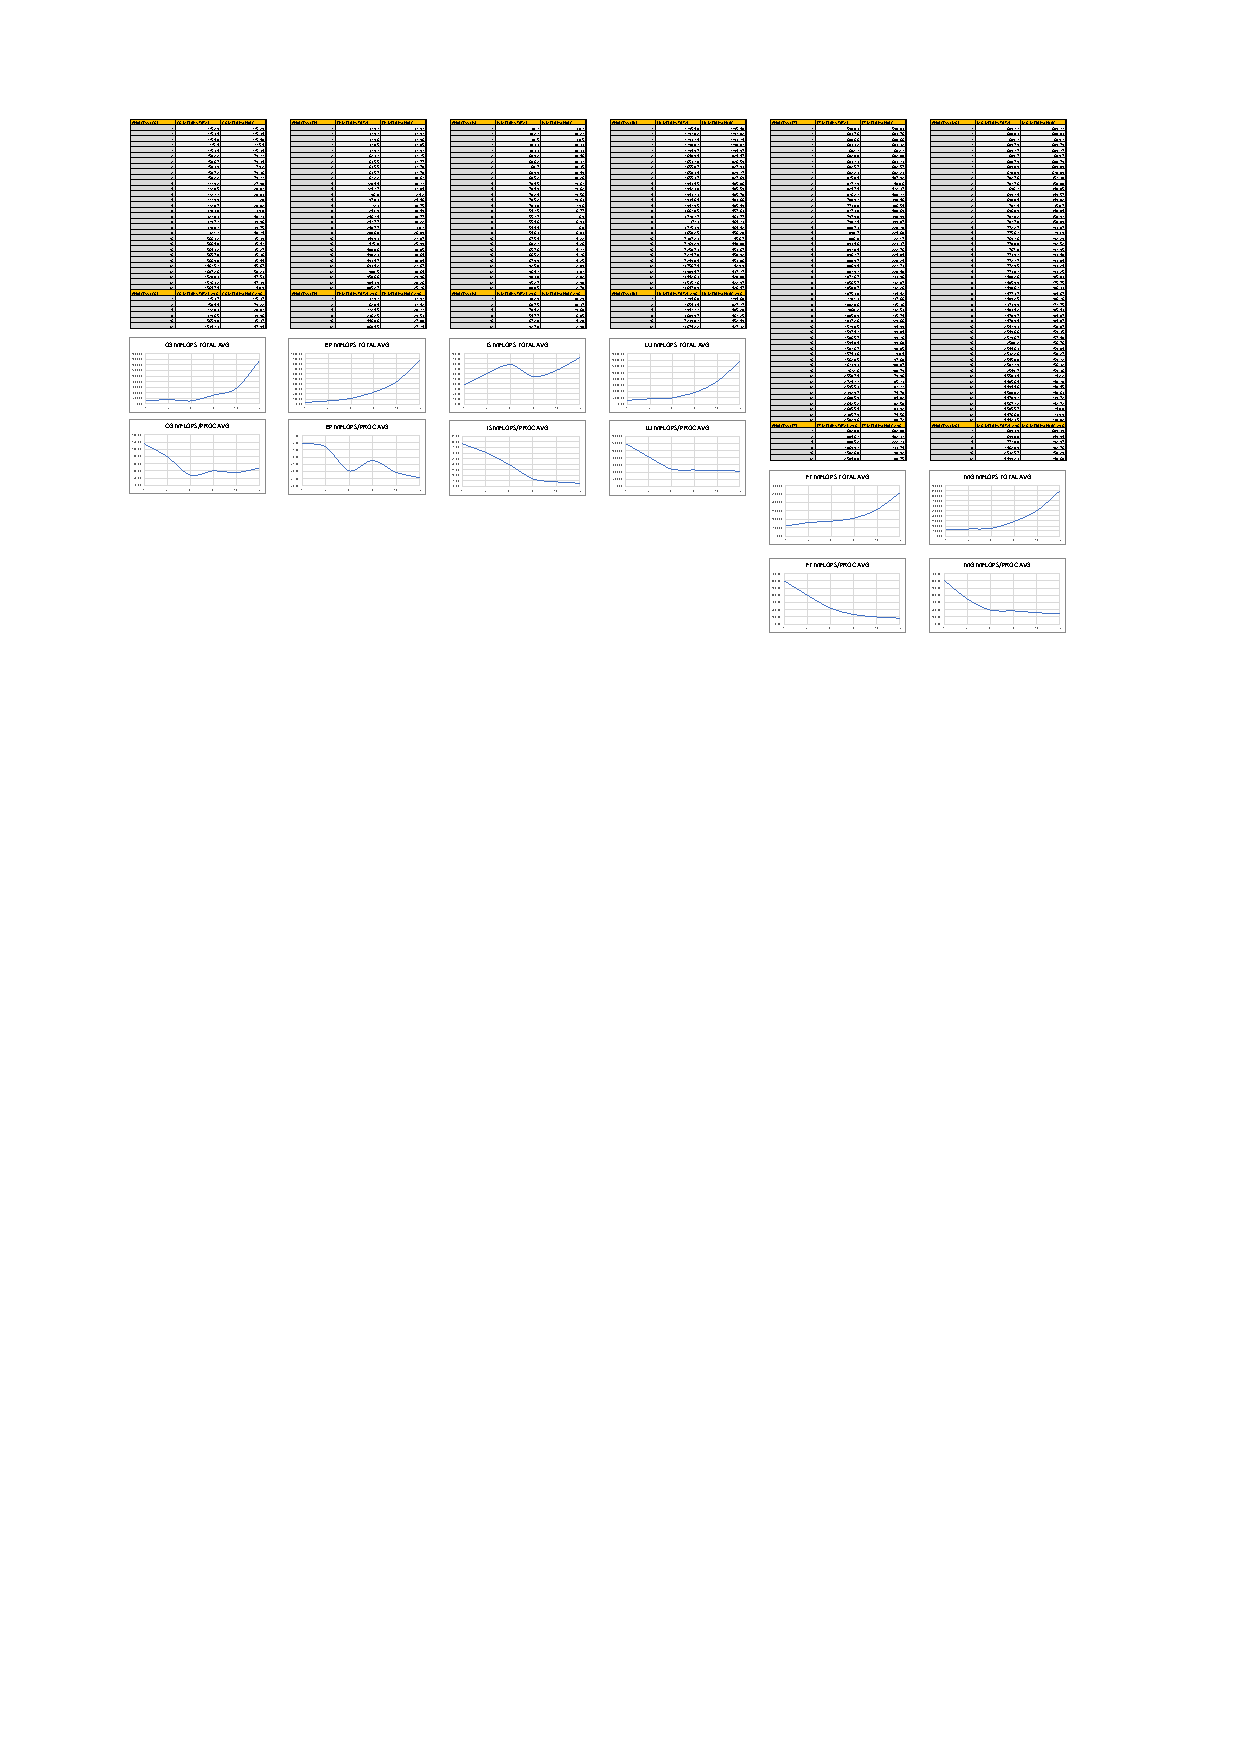
\includepdf[landscape,trim=02mm 190mm 10mm 20mm]{pdf_tex/bench_values/values.pdf}
\chapter{Presupuesto de Clúpiter}
\label{chap:presupuesto_clupiter}

\lettrine{E}{n} la siguiente página se adjunta una copia del presupuesto de Clúpiter. A éste hay que añadir los cables magnéticos comprados posterioremente:

\begin{figure}[H]
  \centering
  \vspace{0.5cm}
  % Left Bottom Right Top
  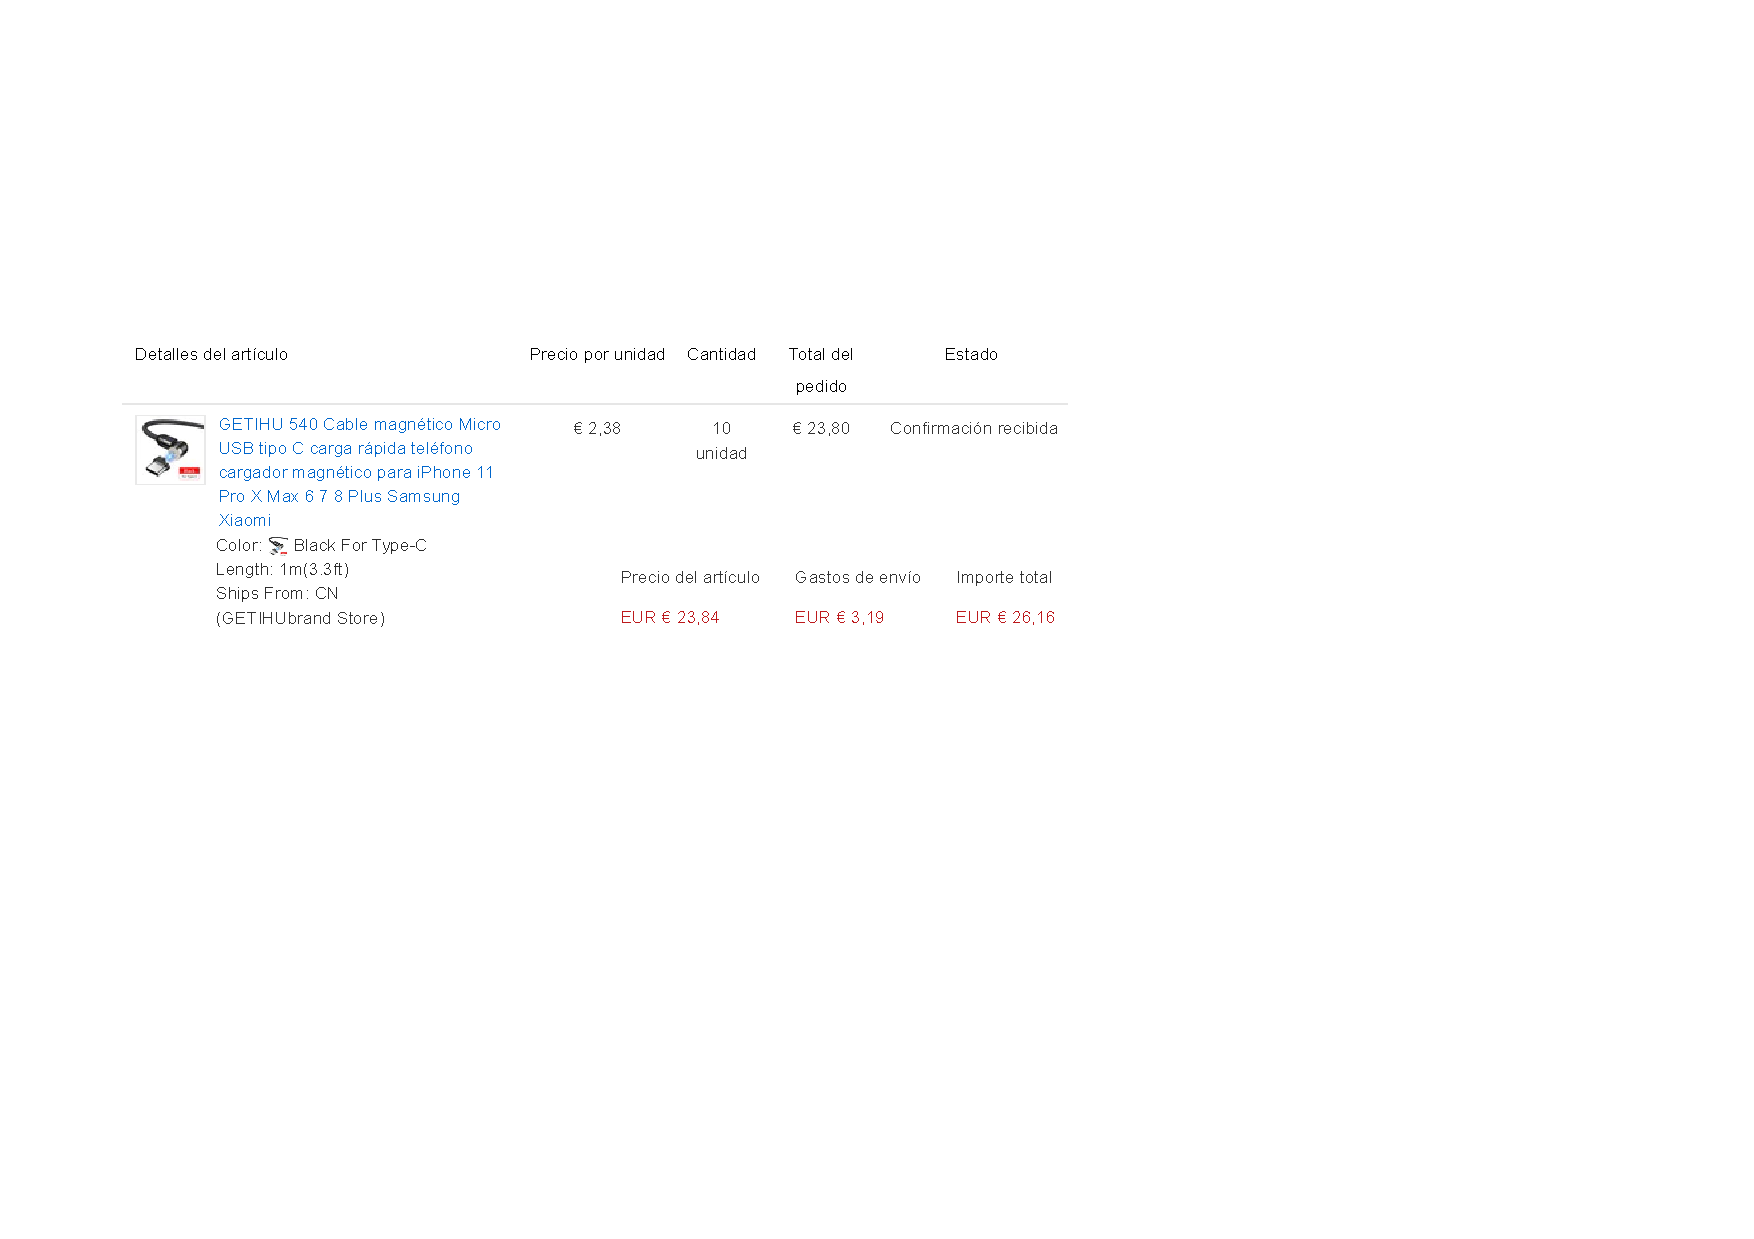
\includegraphics[width=\textwidth,trim=18mm 98mm 113mm 57mm]{pdf_tex/presupuesto_clupiter/getihu_cable.pdf}
\end{figure}

% Left Bottom Right Top
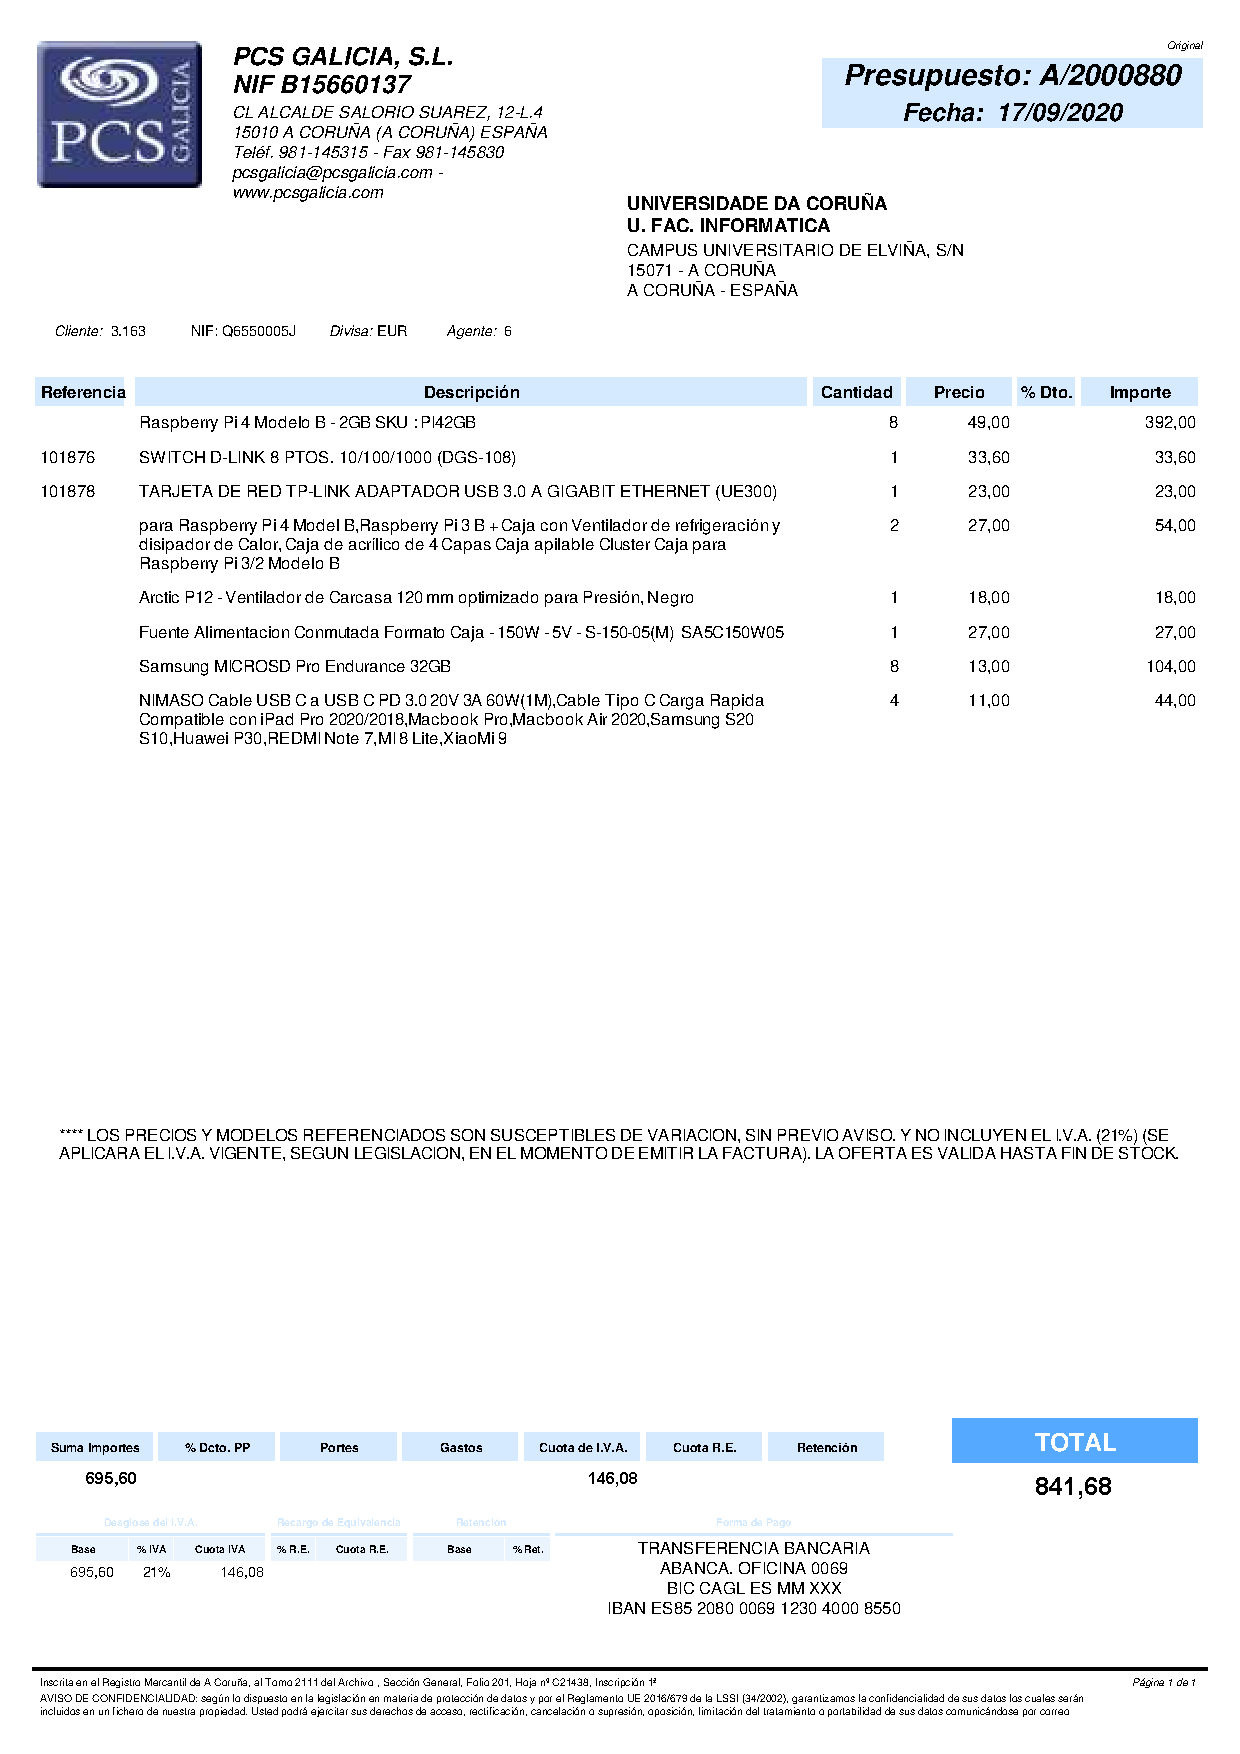
\includepdf[]{pdf_tex/presupuesto_clupiter/Presupuesto_PCS_Galicia_(C).pdf}
\chapter{Guía de mantenimiento de Arch Linux}
\label{chap:archlinux_maintenance_guide}

\lettrine{E}{n} este apéndice se encuentra una breve guía de los comandos más básicos para mantener Clúpiter a punto, especialmente haciendo enfoque en las actualizaciones y mantenimiento básico del sistema.

\section{Enlaces de interés}
Ante cualquier duda, consulta, o problema, se debe acudir a la wiki de Arch Linux, donde lo más probable es que se encuentre la respuesta. A continuación se muestra una lista de entradas relevantes de esta wiki y similares:

\begin{itemize}
    \item Introducción a Arch Linux, donde en especial se recomienda la sección ``Package management''.
    \url{https://wiki.archlinux.org/title/General_recommendations}

    \item Arch User Repository. Este es un repositorio gestionado por la comunidad, donde se pueden encontrar gran cantidad de paquetes no soportados oficialmente, pero que habitualmente cuentan con un soporte de calidad. En caso de emplearse de forma asidura, se recomienda instalar un \textit{wrapper} de AUR, como por ejemplo \texttt{yay} o \texttt{paru}.\\
    \url{https://wiki.archlinux.org/title/Arch_User_Repository}

    \item Manual para systemd: \url{https://wiki.archlinux.org/title/Systemd}.
    \item Configuración de red: \url{https://wiki.archlinux.org/title/Systemd-networkd}.
    \item Configuraciones para \acrlong{rpi}: \\\url{https://archlinuxarm.org/wiki/Raspberry_Pi}.

    \item Manual de pacman, el gestor de paquetes de Arch Linux: \\\url{https://wiki.archlinux.org/title/General_recommendations}
\end{itemize}

Para un usuario más novato esto podría parecer abrumados en un principio, pero desde mi punto de vista esta la mejor forma de aprender, y el espíritu que promueve Arch Linux. 

\section{Actualización del sistema}
Si se han leido con detenimiento las entradas en la sección anterior no debería haber mucha duda en qué hacer para actualizar el sistema. Sin embargo, siembre vienen bien las recomendaciones basadas en la experiencia.

Como Clúpiter probablemente se actualice muy de vez en cuando, es necesario tomar precauciones para evitar posibles comportamientos indeseados tras la actualización. De esta forma, estando conectados a internet, y por este orden, se debe ejecutar en todos los nodos:

\begin{enumerate}
    \item Hacerse superusuario.
\begin{lstlisting}[language=bash]
su -
\end{lstlisting}
    \item Actualizar la base de datos de pacman:
\begin{lstlisting}[language=bash]
pacman -Syy
\end{lstlisting}
    \item Actualizar los llaveros de claves, o \textit{keyring}:
\begin{lstlisting}[language=bash]
pacman -S archlinux-keyring archlinuxarm-keyring
\end{lstlisting}
    \item Visualizar el resto de actualizaciones con:
\begin{lstlisting}[language=bash]
pacman -Syu
\end{lstlisting}
    \textbf{NOTA:} Los servidores de ArchLinuxARM no parecen ser los mejores, por lo que a veces puede dar error al descargar algún archivo. En ese caso, no hay de qué preocuparse: \texttt{pacman -Syu} es idempotente, y se puede ejecutar todas las veces requeridas hasta que se descarguen todos los paquetes. Aún así, es conveniente esperar un pequeño tiempo por si el servidor está experimentando dificultades técnicas transitorias.
    
    \item Verificar las versiones de las actualizaciones, \textbf{especialmente las que cambien de versión mayor}, esto es, de php 7 a php 8, por ejemplo. Si hubiera alguna actualización mayor, es conveniente hacer una búsqueda en internet para verificar que no haya incompatibilidades.
    Por ejemplo, en el caso de php, se buscaría ``php 8 update arch linux'', y entre los primeros resultados se encuentra: \\\footnotesize\url{https://archlinux.org/news/php-80-and-php-7-legacy-packages-are-available/}\normalsize

    Además es muy conveniente verificar las noticias en la sección principal de \url{https://archlinux.org}, donde suelen dar la solución a los problemas que se puedan encontrar durante la actualización, especialmente en el caso de que algún paquete sea eliminado, sustituído por otro, o haya algún problema de dependencias derivado de las situaciones anteriores.

    \item Finalmente, proceder y realizar la actualización pulsando \texttt{Y}, \texttt{S}, o \texttt{<ENTER>} (esta última acepta la letra en mayúscula, lo cual es habitualmente la mejor idea). Es recomendable reiniciar tras una actualización del kernel, lo cual es algo probable si éstas se realizan cada bastante tiempo.
\end{enumerate}

\subsection{Asciinema}
En la dirección \url{https://asciinema.org/a/434085}, se puede ver el proceso de actualización de uno de los nodos de Clúpiter. Recordar que esta acción debe llevarse a cabo simultáneamente en todos los nodos, por ejemplo, con el programa terminator, como se ve en la Figura \ref{fig:terminator_update}. Además, el archivo grabado se puede encontrar en el repositorio del proyecto bajo la carpeta \texttt{doc/asciinema}, y se puede reproducir con el comando \texttt{asciinema play archlinux-update.cast}.

\begin{figure}[h!]
  \centering
  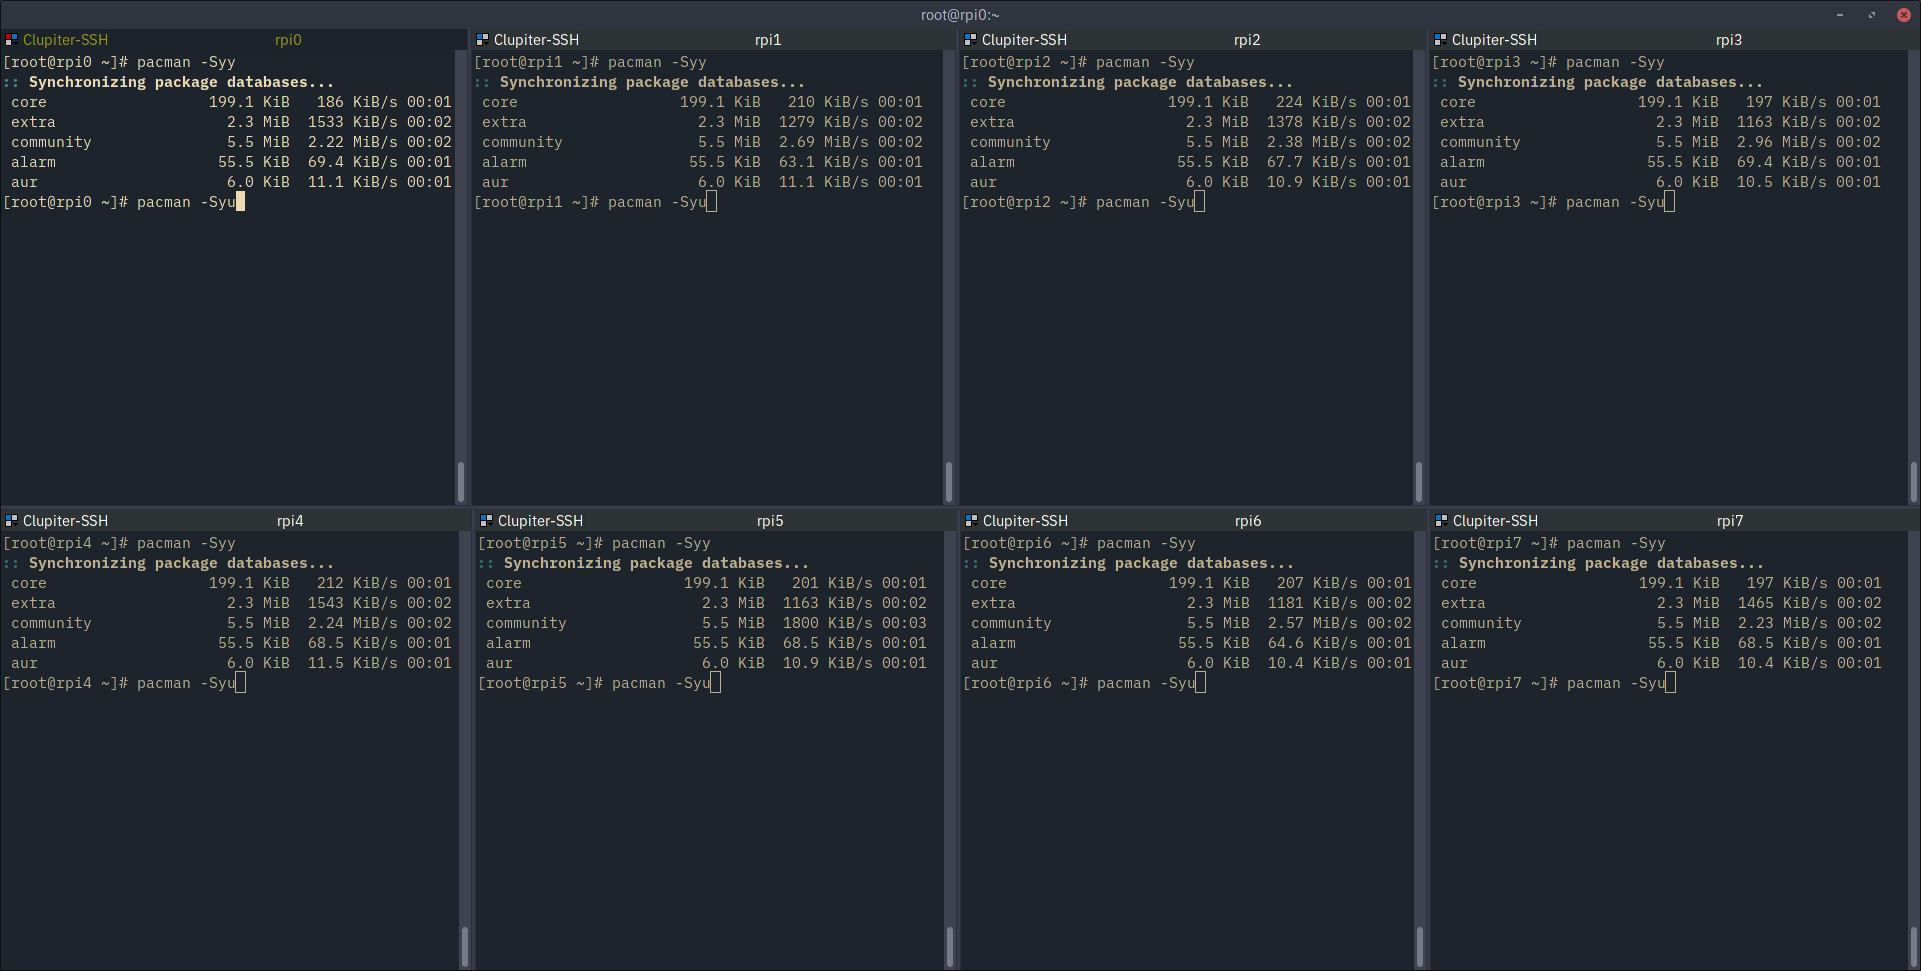
\includegraphics[width=\textwidth]{img/terminator_update.png}
  \caption{Operación en paralelo de Clúpiter con terminator}
  \label{fig:terminator_update}
\end{figure}
%\include{anexos/...}

\printglossary[type=\acronymtype,title=\nomeglosarioacronimos]
\printglossary[title=\nomeglosariotermos]

\bibliographystyle{IEEEtranN}
\bibliography{\bibconfig,bibliografia/bibliografia}
\cleardoublepage

\end{document}

%%%%%%%%%%%%%%%%%%%%%%%%%%%%%%%%%%%%%%%%%%%%%%%%%%%%%%%%%%%%%%%%%%%%%%%%%%%%%%%%
